%
% Modelo para Capa final de tese de doutoramento
% do MEI.
%
% Incorpora elementos impostos pelo Regulamento de Estudos Pos-Graduados da
% Universidade de Lisboa (DR: 31/08/2017)
%
\documentclass[
 paper=A4,               % paper size --> A4 is default in Germany
    twoside=true,           % onesite or twoside printing
    openright,              % doublepage cleaning ends up right side
    parskip=full,           % spacing value / method for paragraphs
    chapterprefix=true,     % prefix for chapter marks
    11pt,                   % font size
    headings=normal,        % size of headings
    bibliography=totoc,     % include bib in toc
    listof=totoc,           % include listof entries in toc
    titlepage=on,           % own page for each title page
    captions=tableabove,    % display table captions above the float env
    draft=false,            % value for draft version
]{scrreprt}

%\DeclareOldFontCommand{\bf}{\normalfont\bfseries}
\usepackage{newstyle}
\usepackage{tabularx}
\usepackage[utf8]{inputenc}
\usepackage{amsmath,amsfonts,amssymb,amsthm,url}
\usepackage[portuguese,english]{babel}
\usepackage{times}
\usepackage{xspace}
\usepackage{setspace}
\usepackage[show]{chato-notes}
\usepackage[sort&compress,numbers]{natbib}
\usepackage[vlined,ruled,commentsnumbered,linesnumbered]{algorithm2e} 
\usepackage{graphicx,multirow}
\usepackage{array}
\usepackage{mathptmx} % use Times in math mode
\usepackage{moreverb}
\usepackage{lscape,rotating}
\usepackage{hyperref}
\usepackage{fancyhdr}
\usepackage{lastpage}
\usepackage{listings}
%\usepackage[tocloft]
\usepackage{subfig}
\usepackage{tikz}
\usepackage{xcolor}
\usepackage{makeidx}

\definecolor{codegreen}{rgb}{0,0.6,0}
\definecolor{codegray}{rgb}{0.5,0.5,0.5}
\definecolor{codepurple}{rgb}{0.58,0,0.82}
\definecolor{backcolour}{rgb}{0.95,0.95,0.92}

\lstdefinestyle{mystyle}{
    backgroundcolor=\color{backcolour},
    commentstyle=\color{codegreen},
    keywordstyle=\color{blue},
    keywordstyle={[2]\color{magenta}},
    numberstyle=\tiny\color{codegray},
    stringstyle=\color{codepurple},
    basicstyle=\footnotesize,
    comment=[l]{\%},
    keywords={@relation,@attribute,@data,modifyvm, do, Vagrant, configure, id},
    morekeywords=[2]{real,integer,numeric,string,date,provider,customize,gui,v,provision, config,vm,box,ssh,insert_key,network},
    breakatwhitespace=false,
    breaklines=true,
    captionpos=b,
    keepspaces=true,
    numbers=left,
    numbersep=5pt,
    showspaces=false,
    showstringspaces=false,
    showtabs=false,
    tabsize=1
}

\lstset{style=mystyle}


\newtheorem*{validity}{Validity}{}
\newtheorem*{liveness}{Liveness}{}
\newtheorem*{security}{Compliance}{}
\newtheorem*{resilience}{Resilience}{}
\newtheorem{definition}{Definition}[]
\newtheorem{assumption}{Assumption}[]

\newcommand{\sender}{\emph{sender-SQ}\xspace}
\newcommand{\Sender}{\emph{Sender-SQ}\xspace}
\newcommand{\senders}{\emph{sender-SQs}\xspace}
\newcommand{\Senders}{\emph{Sender-SQs}\xspace}
\newcommand{\presieve}{\emph{pre-SQ}\xspace}
\newcommand{\Presieve}{\emph{Pre-SQ}\xspace}
\newcommand{\Presieves}{\emph{Pre-SQs}\xspace}
\newcommand{\presieves}{\emph{pre-SQs}\xspace}
\newcommand{\repsieve}{\emph{replica-SQ}\xspace}
\newcommand{\Repsieve}{\emph{Replica-SQ}\xspace}
\newcommand{\repsieves}{\emph{replica-SQs}\xspace}
\newcommand{\Repsieves}{\emph{Replica-SQs}\xspace}
\newcommand{\postsieve}{\emph{post-SQ}\xspace}
\newcommand{\Postsieve}{\emph{Post-SQ}\xspace}

\newcommand{\msg}{\texttt{Msg}\xspace}
\newcommand{\sn}{\emph{sn}\xspace}
\newcommand{\signature}{\emph{sgn}\xspace}
\newcommand{\mac}{\emph{mac}\xspace}
\newcommand{\senderi}{\emph{S}\xspace}
\newcommand{\sendersqi}{\emph{SQ}\xspace}
\newcommand{\presievei}{\emph{PS}\xspace}
\newcommand{\replicak}{\emph{RS}\xspace}
\newcommand{\postsievej}{\emph{PQ}\xspace}
\newcommand{\receiverj}{\emph{R}\xspace}
\newcommand{\privkey}{\emph{prk}\xspace}
\newcommand{\pubkey}{\emph{puk}\xspace}
\newcommand{\sharedkey}{\emph{shk}\xspace}


\newcommand{\system}{\textsc{Lazarus}\xspace}
\newcommand{\sieveq}{\textsc{SieveQ}\xspace}
\newcommand{\controller}{\textsc{Baton}\xspace}
\newcommand{\fetcher}{\emph{Data manager}\xspace}
\newcommand{\manager}{\emph{Deploy manager}\xspace}
\newcommand{\risk}{\emph{Risk manager}\xspace}

\newcommand{\block}{\emph{Diversity block}\xspace}
\newcommand{\blocks}{\emph{Diversity blocks}\xspace}
\newcommand{\replica}{\emph{replica}\xspace}
\newcommand{\replicas}{\emph{replicas}\xspace}
\newcommand{\configuration}{\emph{System configuration}\xspace}
\newcommand{\configurations}{\emph{System configurations}\xspace}
\newcommand{\configurationClean}{System configuration}


\SetKwData{RS}{\texttt{POOL}}
\SetKwData{ES}{\texttt{CONFIG}}
\SetKwData{SC}{\texttt{RAND\_CONFIG}}
\SetKwData{PS}{\texttt{CANDIDATES}}
\SetKwData{RM}{\texttt{REMOVABLES}}
\SetKwData{QS}{\texttt{QUARANTINE}}
\SetKwData{COMB}{\texttt{COMB}}
\SetKwData{COMBS}{\texttt{COMBINATIONS}}
\SetKwData{MAX}{\texttt{MAXIMALS}}
\SetKwData{N}{\texttt{N}}
\SetKwData{r}{\texttt{r}}
\SetKwData{K}{\texttt{K}}
\SetKwData{toRemove}{\texttt{toRemove}}
\SetKwData{toJoin}{\texttt{toJoin}}
\SetKwFunction{Rand}{rand}
\SetKwFunction{Monitor}{Monitor}
\SetKwFunction{reset}{resetSets}
\SetKwFunction{patched}{isPatched}
\SetKwFunction{score}{score}
\SetKwFunction{updatepool}{updatePool}
\SetKwFunction{oldestVulnerability}{scoreAVG}
\SetKwFunction{Risk}{risk}
\SetKwFunction{Replace}{updateSets}
\SetKwProg{Fn}{Function}{}{}

\makeindex



\theoremstyle{definition}
\newtheorem{defn}{Definition}[]

\newcommand*\circled[1]{\tikz[baseline=(char.base)]{
            \node[shape=circle,fill,inner sep=1pt] (char) {\textcolor{white}{#1}};}}

\fancyhf{} %
\lhead{\nouppercase {\leftmark}} %
\rhead{\nouppercase {\bf \thepage}}
\renewcommand{\headrulewidth}{0.1pt}

% Comando para inserir pagina em branco (inserida na numeracao, mas sem
% numero impresso) para quando e' preciso obrigar um capitulo a comecar
% do lado direito (pagina impar)
\newcommand{\LIMPA}{
\newpage
\mbox{}
\thispagestyle{empty}
}

% Igual, mas insere pagina com numero impresso (normalmente nao se usa)
\newcommand{\LIMPAC}{
\newpage
\mbox{}
\thispagestyle{plain}
}

%
% ALTERAR AQUI AS INFORMACOES RELATIVAS AO PROJECTO
%
\newcommand{\TITULO}{DIVERSE INTRUSION-TOLERANT SYSTEMS}
\newcommand{\Autor}{Miguel Garcia Tavares Henriques}
\newcommand{\AutorNumAluno}{35054}

%Orientador e CoOrientador *sem* titulos (e.g. Prof. Doutor)
\newcommand{\Orientador}{Alysson Neves Bessani}
\newcommand{\CoOrientador}{Nuno Fuentecilla Maia Ferreira Neves} %se nao se aplicar, nao importa o que aqui esteja

%Se aplicavel, o supervisor pode ter um titulo (Dr., Eng.) colocado aqui
\newcommand{\SupervisorInstituicao}{Nome Completo do Supervisor}  %se nao se aplicar, nao importa o que aqui esteja

\newcommand{\AnoLectivo}{2017/2018}
\newcommand{\Ano}{\Large{2018}}

% Comentar/descomentar conforme conveniente
\newcommand{\TIPO}{DISSERTA\c{C}\~{A}O }
%\newcommand{\TIPO}{TRABALHO DE PROJETO }

% Comentar/descomentar conforme conveniente
%\newcommand{\MESTRADO}{MESTRADO EM -- PREENCHER --}
\newcommand{\DOUTORAMENTO}{Doutoramento em Inform\'{a}tica}

% Comentar/descomentar conforme conveniente
%\newcommand{\IdiomaTese}{\selectlanguage{portuguese}}
\newcommand{\IdiomaTese}{\selectlanguage{english}}

% Comentar/descomentar conforme conveniente
\newcommand{\Especialidade}{}

\newcommand{\Cabecalho}{
\vspace{1cm}\normalfont\normalfont
\vfill
\textsc{\normalsize\uppercase{Universidade de Lisboa}}\\
\normalsize\uppercase{Faculdade de Ci\^{e}ncias}\\
\vspace{1cm}

\includegraphics[scale=.45]{pic/logo_fcul_vertical.png}\\
}

\usepackage{ifpdf}
\ifpdf
\pdfinfo {
	/Author (\Autor)
	/Title (\TITULO)
	/Subject (\DOUTORAMENTO)
	/Keywords ()
	/CreationDate (D:20081112151803)
}
\fi

%\usepackage[dvips]{geometry}
%\geometry{a4paper=true,portrait=true,left=3cm,right=3cm,top=2.5cm,bottom=3.5cm}

\title{\TITULO}
\author{\Autor}
%\date{\today}

\usepackage{glossaries}
\makeglossaries

\begin{document}
\selectlanguage{english}
\pagestyle{empty}

% Primeira capa
% 
%
\begin{center}

\Cabecalho

\vspace{2.0cm}
\vfill
\IdiomaTese
\Large{\textbf{\TITULO}}\\
\vspace{2cm}
\vfill

\large{\textbf{\DOUTORAMENTO}}\\
%\normalsize{\Especialidade}\\
\vspace{2.0cm}
\vfill
\Large{\textbf{\Autor}}\\
\vspace{1,8 cm}
\vfill
\large{Tese orientada por:}\\
%\normalsize{Trabalho de projeto orientado por:}\\
\large{Prof. Doutor \Orientador} \\
% DESCOMENTAR a linha relevante (se alguma), removendo o % no inicio
e co-orientada pelo Prof. Doutor \CoOrientador \\
\vspace{1 cm}
\vfill

\normalsize{Documento especialmente elaborado para a obten\c{c}\~{a}o do grau de doutor}
\vspace{0.5cm}
\vfill
\Ano
\end{center}
\newpage
\mbox{}
\newpage

%
% Segunda capa
%

\begin{center}

\Cabecalho

\vspace{0.5cm}
\vfill
\IdiomaTese
\Large{\textbf{\TITULO}}\\
\selectlanguage{portuguese}
\vspace{1cm}
\vfill

\large{\textbf{\DOUTORAMENTO}}\\
%\normalsize{\Especialidade }\\
\vspace{1cm}
\vfill
\Large{\textbf{\Autor}}\\
\vspace{.5 cm}
\vfill
\large{Tese orientada por:}\\
%\normalsize{Trabalho de projeto orientado por:}\\
\large{Prof. Doutor \Orientador} \\
% DESCOMENTAR a linha relevante (se alguma), removendo o % no inicio
e pelo Prof. Doutor \CoOrientador \\
\vspace{.3 cm}
\vfill

\begin{flushleft}  
\large{J\'{u}ri}
%\vfill
\setlength{\leftskip}{0.5cm}
\normalsize{Presidente:}
\begin{itemize}
%\setlength\itemsep{-0.3 em}
\item{Nome do Presidente}
\end{itemize}
\normalsize{Vogais:}
\begin{itemize}
\setlength\itemsep{-1 em}
\item{Nome do Vogal}
\item{Nome do Vogal}
\item{Nome do Vogal}
\item{Nome do Vogal}
\end{itemize}
\setlength{\leftskip}{0cm}
\end{flushleft}
\vspace{0.0cm}
%\vfill

\Ano
\end{center}
\newpage
\mbox{}
\newpage

\begin{center}
\normalsize{Documento especialmente elaborado para a obten\c{c}\~{a}o do grau de doutor\par}
\vspace{0.0cm}
\normalsize{Este trabalho foi financiado pela Funda\c{c}\~{a}o para a Ci\^{e}ncia e Tecnologia (FCT) atrav\'{e}s da Bolsa Individual de Doutormento SFRH/BD/84375/2012 e atrav\'{e}s dos projectos da Comiss\~{a}o Europeia FP7-257475 (MASSIF) e H2020-700692 (DiSIEM).}
\vspace{0.cm}
\vfill
\end{center}

% Fim da capa
% ----------------------------------------------------------------------


\pagenumbering{roman}			% roman page numbing (invisible for empty page style)
\pagestyle{empty}				% no header or footers

\cleardoublepage

\pagestyle{plain}				% display just page numbers
% ----------------------------------------------------------------------
% P�gina do resumo em Ingl�s:
% 300 palavras
\selectlanguage{english}
%\vspace*{2cm}
%\begin{center}
%\Large \bf Abstract
%\end{center}
%\vspace*{1cm} \setlength{\baselineskip}{0.6cm}
\chapter*{Abstract}
\label{chapter:abstract_en}
\vspace*{-10mm}

Over the past 20 years, there have been indisputable advances on the development of Byzantine Fault-Tolerant (BFT) replicated systems. 
These systems keep operational safety as long as at most $f$ out of $n$ replicas fail simultaneously. 
Therefore, in order to maintain correctness it is assumed that replicas do not suffer from common mode failures, or in other words that replicas fail independently. 
In an adversarial setting, this requires that replicas do not include similar vulnerabilities, or otherwise a single exploit could be employed to compromise a significant part of the system. 
The thesis investigates how this assumption can be substantiated in practice by exploring diversity when managing the configurations of replicas.

The thesis begins with an analysis of a large dataset of vulnerability information to get evidence that diversity can contribute to failure independence. 
In particular, we used the data from a vulnerability database to devise strategies for building groups of $n$ replicas with different Operating Systems (OS). 
Our results demonstrate that it is possible to create dependable configurations of OSes, which do not share vulnerabilities over reasonable periods of time (i.e., a few years).

Then, the thesis proposes a new design for a firewall-like service that protects and regulates the access to critical systems, and that could benefit from our diversity management approach. 
The solution provides fault and intrusion tolerance by implementing an architecture based on two filtering layers, enabling efficient removal of invalid messages at early stages in order to decrease the costs associated with BFT replication in the later stages.

The thesis also presents a novel solution for managing diverse replicas. 
It collects and processes data from several data sources to continuously compute a risk metric. 
Once the risk increases, the solution replaces a potentially vulnerable replica by another one, 
trying to maximize the failure independence of the replicated service. 
Then, the replaced replica is put on quarantine and updated with the available patches, to be prepared for later re-use. 
We devised various experiments that show the dependability gains and performance impact of our prototype, including key benchmarks and three BFT applications (a key-value store, our firewall-like service, and a blockchain). 

%This thesis addresses the problem of building dependable Byzantine fault-tolerant (BFT) systems through diversity. 
%Although the indisputable contributions of many works from the BFT research community, diversity management still is a long-standing open problem of this area. 
%BFT safety holds under the strict assumption that only $f$ out $n$ replicas fail \emph{simultaneously}.
%Therefore, it is assumed that replicas fail independently (e.g., they do not share vulnerabilities).
%Otherwise, the amount of effort to compromise $f$ replicas would be the same as to compromise $f+1$, becoming easier to break the BFT safety.


%The thesis begins with an analysis (that is in some part prior to this thesis) on security data.
%This analysis shows evidence to support failure independence among BFT replicas.
%In particular, we used a vulnerability database to build sets of $n$ replicas with different Operating Systems (OS).
%Based on these results, it is possible to create dependable configurations of OSes of BFT systems. 


%Nevertheless, we have identified some limitations on the previous analysis. 
%These were mainly due to missing data that would provide inaccurate results.
%Therefore, we designed a more advanced solution to manage the diversity of any BFT system. 
%We developed a solution that considers several (free) security data sources.
%This data, feeds a novel metric that is used to make decisions on diversity sets minimizing the common vulnerabilities.
%We developed a methodology to address off-the-shelf diversity in general. 
%However, here we focused on OSes as there resides the replica's major code complexity.
%Moreover, we extended this contribution in a more practical way and developed a prototype that enables automatic management of BFT replicas' diversity.
%Hence, we reduce the complexity inherent from dealing with diverse software in replicated systems. 

%We devised a few experiments that show the dependability gains of using an advanced diversity selection and the impact of using different OSes in a few BFT applications (one of them is a BFT firewall-like that is part of the contributions of this thesis).
%Nevertheless, implementation decisions made us pay an additional cost on the performance to achieve such results on dependability.

\vfill

\begin{flushleft}
\textbf{Keywords:}
Diversity, Vulnerabilities, Operating Systems, Intrusion Tolerance, Rejuvenations.
\end{flushleft}

%\LIMPA

% Fim da p�gina do resumo em Ingl�s.
% ----------------------------------------------------------------------

\cleardoublepage

\pagestyle{plain}				% display just page numbers
%\pagestyle{empty}

% ----------------------------------------------------------------------
% P�gina do resumo em Portugu�s:
\selectlanguage{portuguese}
\chapter*{Resumo}
\label{chapter:abstract_pt}
\vspace*{-10mm}


\vfill

\begin{flushleft}
\textbf{Palavras-chave:}
Diversidade, Vulnerabilidades, Sistemas Operativos, Toler\^{a}ncia a Intrus\~{o}es, Recuper\c{c}\~{a}o Proactiva.
\end{flushleft}

\LIMPA
% Fim da p�gina do resumo em Portugu�s
% ----------------------------------------------------------------------

\cleardoublepage

\pagestyle{plain}				% display just page numbers
%\pagestyle{empty}

% ----------------------------------------------------------------------
% P�gina do resumo em Portugu�s:
\selectlanguage{portuguese}
\chapter*{Resumo Estendido}
\label{chapter:abstract_pt}
\vspace*{-10mm}


\vfill

\begin{flushleft}
\textbf{Palavras-chave:}
Diversidade, Vulnerabilidades, Sistemas Operativos, Toler\^{a}ncia a Intrus\~{o}es, Recuper\c{c}\~{a}o Proactiva.
\end{flushleft}

\LIMPA
% Fim da p�gina do resumo em Portugu�s
% ----------------------------------------------------------------------

\cleardoublepage

\pagestyle{plain}

\vspace*{2cm}
\selectlanguage{portuguese}
\chapter*{Agradecimentos}

%\begin{center}
%\selectlanguage{portuguese}
%\Large \bf Agradecimentos
%\selectlanguage{english}

Este documento encerra todo trabalho feito ao longo de alguns anos desde o mestrado até agora. 
Durante estes anos tive a sorte de trabalhar com dois investigadores de grande qualidade, os meus orientadores Professor Alysson Bessani e Professor Nuno Neves.
Devo-lhes um sincero obrigado por todos os ensinamentos e orientações que me transmitiram. 
Cada um da sua forma contribuiram para o meu crescimento como pessoa e investigador. 

A todos os meus colegas e amigos do LASIGE e DI, aos que vieram e foram e aos que vieram  e ficam, em todas as fases do doutoramente tive rodeado de boa gente. Em especial um agradecimento ao Tiago, Ibéria, Vavala, Eduardo, João, Fernando, André e ao Vinicius. A vossa amizade, companheirismo, compreensão, inter-ajuda e motivação foram essenciais nesta fase.  

A todos os meus amigos fora deste "universo" que de uma forma ou de outra contribuiram para este tese. 
Mesmo sem compreenderem bem o que eu fazia devo-lhes a boa disposição e animo. 
O prêmio de paciência vai para o Bruno, Paulo e Gonçalo.


Sem a minha familia seria impossível chegar ao fim desta maratona. 
Aos de casa e aos que escolhi para serem parte da minha familia.
Em especial à minha mãe, aos meus irmãos Diogo e Joana, à Vanessa e à Ana por serem incansáveis e se hoje sou mais forte é porque tive o vosso apoio.
Obrigado e espero que tenham orgulho em mim. 



%\Large \bf Acknowledgments
%\end{center}
%\vspace*{1cm} \setlength{\baselineskip}{0.6cm}



\LIMPA
\LIMPA

\vfill

%\selectlanguage{portuguese}

\begin{flushright}\textit{Para a minha avó.}\end{flushright}

\LIMPA

\cleardoublepage
%
\setcounter{secnumdepth}{1}
\setcounter{tocdepth}{2}		% define depth of toc


%Lista de capitulos
\tableofcontents				% display table of contents
%\addcontentsline {toc} {chapter} {Content}
\newpage
\thispagestyle{empty}
\mbox{}
\newpage


%Lista de figuras
\listoffigures
\addcontentsline {toc} {chapter} {List of Figures}
\newpage
\thispagestyle{empty}
\mbox{}
\newpage

%Lista de tabelas
\listoftables
\addcontentsline {toc} {chapter} {List of Tables}
\newpage
\thispagestyle{empty} \mbox{}
\newpage

% --------------------------
% Body matter
% --------------------------
\pagenumbering{arabic}			% arabic page numbering
\setcounter{page}{1}			% set page counter
\pagestyle{maincontentstyle} 	% fancy header and footer


% ----------------------------------------------------------------------
% Inicio conteudo
%\pagestyle{fancy}
%\cleardoublepage

%\setcounter{page}{1}
%\pagenumbering{arabic}

\chapter{Introduction}
\label{chap:introduction}

\section{Context and Motivation}
\gls{bft}\footnote{In this thesis we interchange Byzantine fault tolerance (subject) with Byzantine fault-tolerant (adjective) using the same acronym BFT for both.} is a well-established area of research that aims to guarantee safety on replicated systems even in the presence of some (Byzantine) faulty nodes.
In a nutshell, \gls{bft} protocols guarantee that replicas agree on the order of the message execution, and thus, the replicas work as a replicated state machine.
The overall \gls{bft} safety holds even if a subpart of replicas, typically $f$ out of $n$, is faulty, leaving a sufficient number of correct nodes that execute correctly.
Although not explicit, this assumption leverages on the strict condition that nodes (must) fail independently.
Otherwise, compromising $f$ replicas is virtually the same as compromising $f+1$.


\gls{bft} was first proposed in 1982 by Lamport~\etal{}~\cite{Lamport:1982}, but it only as awaken the distributed systems research community to its relevancy in 1999 due to Castro and Liskov's Practical \gls{bft}~\cite{Castro:1999}. 
In the last twenty years of active research on \gls{bft} replication, there were made great advances on the performance (e.g.,~\cite{Kotla:2010,Aublin:2015,Behl:2015}), use of resources (e.g.,~\cite{Yin:2003,Wood:2011,Veronese:2013,Liu:2016,Behl:2017}), and robustness (e.g.,~\cite{Amir:2011,Bessani:2014,Clement:2009b}) of \gls{bft} systems.
However, \gls{bft} in general and these works in particular, assume, either implicitly or explicitly, that the replica nodes fail independently. 
This assumption extends the fault threshold as it considers that it takes more time/effort to compromise replicas that do not share vulnerabilities.
Nevertheless, a few works rely on some orthogonal mechanisms (e.g.,~\cite{Roeder:2010,Chen:1995}) to avoid these common weaknesses, or rule out the possibility of malicious failures from their system models.
Moreover, a few works have implemented and experimented with such mechanisms (e.g.,~\cite{Rodrigues:2001,Roeder:2010,Amir:2011}), but in a very limited way.


In practice, a few dependable applications take advantage of diversity mechanism. 
Nevertheless, in these cases, diversity is applied \emph{intuitively}.
For example, in avionics engineering, a few aircraft solutions embrace the diversity of components to avoid accidental failures~\cite{Yeh:2004}.
Moreover, in 2014, the U.S. Navy developed the Resilient Hull, Mechanical, and Electrical Security (\textsc{Rhimes}), it introduces diversity through a \emph{slightly different implementation} for each programmable logic controller~\cite{rhimes}.
Another example of a critical system that naturally adopted diversity are the \gls{dns} root servers. 
According to Lars-Johan Liman (the technical lead of one of the \gls{dns} root servers),\footnote{https://www.netnod.se/dns/dns-root-server-faq} each operator has its own configurations, as ``\emph{it allows for great operational diversity. That means, for example, that a single software or firmware bug cannot bring down the entire system}.''
\textbf{FIX THIS} On the contrary, the growing blockchain technology implements \gls{bft} in a large and dispersed network.
The proof-of-work~\cite{} solutions do not need a strictly bounded fault threshold, as their threshold is bounded by 51\% of the network is correct.


Despite the adoption of (naive) diversity in practical systems, other variables must be considered to make systems dependable and secure.
For example, even considering an initial set of $n$ diverse replicas, long-running services need to be cleaned from possible failures and intrusions.
A few works on the proactive recovery of \gls{bft} systems~\cite{Castro:2002,Sousa:2010,Roeder:2010,Platania:2014,Distler:2011} periodically restart their replicas to clean undetected faulty states introduced by a stealth attacker. 
However, these works (i) assume replicas failure independence, (ii) do not provide proof to support their diversity decisions or (iii) use limited solutions (e.g., memory randomization).
Therefore, unless careful selection of diversity is introduced during recoveries, the replicas do not change, thus keeping the same vulnerabilities.


Finally and despite the already established maturity of \gls{bft} solutions, no one debated how to apply diversity in a dependable (i.e., which software configurations are more dependable) and when should these configurations be changed (e.g., recovering replicas with different software).

\section{Objectives and Contributions}

In the past, several researchers developed and improved techniques to make intrusion tolerance a cornerstone of security and dependability.
Nevertheless, a few problems were left open and still lack effective answers.
This thesis aims to push forward intrusion tolerance to more accurate and practical grounds.
The main contributions of this thesis are summarized into the following points, along with the related publications.


\subsection{Evidence for Implementing Diversity}% Diversity Study on Off-the-Shelf Operating Systems}


The results achieved during the MSc thesis encouraged us to extend the work on the diversity of \gls{ots} \glspl{os}~\cite{Garcia:2012}.
This first step towards the design and development of dependable \gls{bft} systems is to assess how accurate were the implicit or explicit assumptions on diversity (e.g.,~\cite{Abd-El-Malek:2005,Bessani:2008,Castro:2002,Castro:2003,Clement:2009,Correia:2004,Kapitza:2012,Kotla:2010,Moniz:2011,Yin:2003}).
In that previous work, we studied the vulnerability data from the \gls{nvd}~\cite{nvd} the most complete vulnerability database available to answer, with arguments to support, to the question:
\emph{What are the dependability gains from using diverse \glspl{os} on a replicated  intrusion-tolerant system?} 
Nevertheless, we have made some extensions to that work, which are presented in this thesis.
In particular, we devised three manual strategies for selecting diverse software components to minimize the incidence of common vulnerabilities in replicated systems.
Moreover, we observed that using different \gls{os} releases of the same \gls{os} is enough to warrant its adoption as a more straightforward, less complicated, more manageable configuration for replicated systems.
The described contributions (together with the ones published during the MSc~\cite{Garcia:2012}) are reported in the following publication:

\begin{enumerate}
\item[1.] \textbf{Analysis of Operating System Diversity for Intrusion Tolerance}, Miguel Garcia, Alysson Bessani, Ilir Gashi Nuno Neves, and Rafael Obelheiro, in \emph{Software: Practice and Experience, 2014}~\cite{Garcia:2014}.
\end{enumerate}



\subsection{Applying Diversity on BFT Systems}
In our first attempt to validate diversity, we presented substantial evidence to claim that using different \glspl{os} guarantees failure independence to some extent.
However, this preliminary analysis suffer from some limitations as other works using \gls{nvd} database (e.g.,~\cite{Gorbenko:2011,Han:2009,Frei:2010,Shahzad:2012,Bozorgi:2010,Allodi:2014,Gorbenko:2017}).
It is possible to find vulnerabilities in \gls{nvd} that are not reported to all affected \glspl{os}.
We have found these missing vulnerabilities reported on other sources (e.g., the vendors' security advisories).
Therefore, some of the results of \gls{nvd}-based studies may provide less accurate conclusions about selecting different software based on common vulnerabilities.
Moreover, \gls{nvd} lacks from some relevant data concerning exploits and patches that are relevant when considering vulnerabilities life-cycle.
An alternative way to \gls{ots} diversity is to generate diversity through automatic mechanisms (e.g.,~\cite{Roeder:2010,Amir:2011}).
However, these mechanisms lack of evidence to claim that these techniques create real vulnerability independence~\cite{Snow:2013,Bittau:2014}. 
Finally, the existent systems that implement time-triggered recoveries assume that it takes the same time/effort to compromise each replica, by assuming that vulnerabilities are all the same. 
This assumption is unrealistic, especially when the replicas' diversity is considered~\cite{Nayak:2014}. 
Therefore, tailored methods are required to evaluate the risk of a replicated system becoming vulnerable (i.e., $f+1$ replicas suffer from the same weaknesses).


In this thesis, we address these problems from both a theoretical and practical perspective.
We address the problems of \emph{finding evidence for supporting diversity}, \emph{manage diversity in a dependable way}, and \emph{support diversity practical mechanisms} in the thesis main contribution.
First, suppress the limitations of \gls{nvd} using clustering techniques, that group similar vulnerabilities, which potentially can be affected by (variations of) the same exploit.
Moreover, we add additional \gls{osint} data sources to build a complete knowledge base about the possible vulnerabilities, exploits, and patches related to the systems of interest. 
The clusters and the collected data are used to assess the risk of a \gls{bft} system becoming compromised by the existence of common vulnerabilities.
Once the risk increases, the system replaces the potentially vulnerable replica by another one, to maximize the failure independence of the replicated service.
The solution continuously collects data from the online sources and monitors the risk of the \gls{bft} in such a way that removes the human from the loop.

We have implemented these contributions in \system, and it is the first system that automatically changes the attack surface of a \gls{bft} system in a dependable way.
\system continuously collects security data from several \gls{osint} feeds to build a vulnerability knowledge base.
This data is used to create clusters of similar vulnerabilities.
These clusters and other collected attributes are used to analyze the risk of the \gls{bft} system becoming compromised. 
Once the risk increases, \system replaces the potentially vulnerable replica by another one, trying to maximize the failure independence. 
The replica's replacement is made automatically, while a new replica is deployed in the \gls{bft} group, the replaced node is put on quarantine and updated with the available patches, to be re-used later.
These mechanisms were implemented to be fully automated and transparent to \gls{bft} systems.
Moreover, the current implementation of \system manages 17 \gls{os} versions, supporting the \gls{bft} replication of a set of representative applications.
The replicas run in \glspl{vm}, allowing provisioning mechanisms to configure them. 
We conducted two sets of experiments: The first one demonstrates that \system risk management can prevent a group of replicas from sharing vulnerabilities over time; 
The second one, reveals the potential negative impact that virtualization and diversity can have on performance. 
In this experiment, we evaluated \system with three \gls{bft} use case applications: (1) a Key-Value Store application, (2) \sieveq an application-like firewall (this contribution is presented in the next section), and (3) a \gls{bft} ordering service for Hyperledger Fabric a blockchain application.
The overall results show that if naive configurations are avoided, \gls{bft} applications in diverse configurations can perform close to our homogeneous bare metal setup.

The contributions of this work resulted in the following publications:

\begin{enumerate}

\item[2.] \textbf{\textsc{Diversys}: DIVErse Rejuvenation SYStem}, Miguel Garcia, Nuno Neves, and  Alysson Bessani in the \emph{Simp\'{o}sio Nacional de Inform\'{a}tica (INFORUM), 2012~\cite{Garcia:2012b}}.


\item[3.] \textbf{Towards an Execution Environment for Intrusion-Tolerant Systems}, Miguel Garcia, Alysson Bessani, and Nuno Neves, Poster session in the \emph{European Conference on Computer Systems (EuroSys), 2016}~\cite{Garcia:2016b}.


\item[4.] \textbf{\system: Automatic Management of Diversity in BFT Systems}, Miguel Garcia, Alysson Bessani, and Nuno Neves -- \emph{Submitted for publication}.

\end{enumerate}


\subsection{BFT Multi-layer Resiliency} 
\system implements mechanisms that provide security and dependability for replicated systems.
However, not all systems need to be \gls{bft}-replicated nor managed with such advanced mechanisms. 
Some of the most critical applications that can benefit from such management are firewalls.
Firewalls are used as the primary protection against external threats, controlling the traffic that flows in and out of a network. 
Typically, they decide if a packet should go through (or be dropped) based on the analysis of its contents. 
Most generic firewall solutions suffer from two inherent problems: 
First, they have vulnerabilities as any other system, and as a consequence, they can also be the target of advanced attacks. 
For example, the \gls{nvd}~\cite{nvd} shows that there have been many security issues in commonly used firewalls. 
\gls{nvd}'s reports present the following numbers of security issues between 2010 and 2018:\footnote{To the date of Jul 12$^{th}$ 2018.} 205 for the Cisco Adaptive Security Appliance; 123 in Juniper Networks solutions; and 50 related to iptables/netfilter. 
Common protection solutions often have been the target of malicious actions as part of a wider scale attack (e.g., anti-virus software~\cite{Chauhan:2011}, \gls{ids}~\cite{Anderson:2001} or firewalls~\cite{Kamara:2003,Surisetty:2010,cisco1,cisco2}).
Second, firewalls are typically a single point of failure, which means that when they crash, the ability of the protected system to communicate may be compromised, at least momentarily.
Therefore, ensuring the correct operation of the firewall under a wide range of failure scenarios becomes imperative.


This last contribution addresses the previously described problems with a new protection system, called \sieveq.
This system mixes the firewall paradigm with a message queue service.
In the last decade, several significant advances occurred in the development of intrusion-tolerant systems.
However, to the best of our knowledge, very few works proposed intrusion-tolerant protection devices, such as firewalls.
Performance reasons might explain this, as \gls{bft} replication protocols are usually associated with significant overheads and limited scalability.
Additionally, achieving complete transparency to the rest of the system can be challenging to reconcile with the objective of having fast message filtering under attack.
In \sieveq, we explore a different design for replicated protection devices, where we trade some transparency on senders and receivers for a more efficient and resilient firewall solution.
In particular, we propose an architecture in which critical services and devices can only be accessed through a message queue and implement the application-level filtering in this queue.
It is assumed that these services have a limited number of senders, which can be appropriately configured to ensure that only they are authorized to communicate through \sieveq.
The solution has a fault- and intrusion-tolerant architecture that applies filtering operations in two stages acting like a sieve.
The first stage, called \emph{pre-filtering}, performs lightweight checks, making it efficient to detect and discard malicious messages from external adversaries.
In particular, messages are only allowed to go through if they come from a pre-defined set of authenticated senders.
\gls{dos} traffic from external sources is immediately dropped, preventing those messages from overloading the next stage.
The second stage, named \emph{filtering}, enforces more refined application level policies, which can require the inspection of some message fields or need the enforcement of specific ordering rules.

The contributions of this work resulted in the following publications:

\begin{enumerate}
\item[5.] \textbf{An Intrusion-Tolerant Firewall Design for Protecting SIEM Systems}, Miguel Garcia, Nuno Neves, Alysson Bessani, in the \emph{Workshop on Systems Resilience in conjunction with the IEEE/IFIP International Conference on Dependable Systems and Networks, 2013}~\cite{Garcia:2013}.

\item[6.] \textbf{\sieveq: A Layered BFT Protection System for Critical Services}, Miguel Garcia, Nuno Neves, and Alysson Bessani, in \emph{IEEE Transactions on Dependable and Secure Computing, 2018}~\cite{Garcia:2016}.
\end{enumerate}


\paragraph{Non-related contributions.}
To conclude, a collaboration with a colleague resulted in a work on \gls{scada} system enhanced with \gls{bft} techniques. 
We documented the challenges of building such system from a ``traditional'' non-\gls{bft} solution.
This effort resulted in a prototype, implemented by the colleague, that integrates the Eclipse NeoSCADA~\cite{eclipsescada} and the \textsc{BFT-SMaRt}~\cite{Bessani:2014} open-source projects.
Although this contribution is out of the scope of the thesis, it is easy to envision the integration of the prototype with \system:


\begin{enumerate}

\item[7.] \textbf{On the Challenges of Building a BFT SCADA}, Andr\'{e} Nogueira, Miguel Garcia, Alysson Bessani, and Nuno Neves, in \emph{Proceedings of the International Conference on Dependable Systems and Networks, 2018 }~\cite{Nogueira:2018}.
\end{enumerate}


\subsection{Thesis Statement}
We summarize our findings in the following thesis statement:

\vspace{2mm}
\fbox{ \begin{minipage}{35em}
\emph{
It is possible to build dependable BFT replicated systems by minimizing the number of replicas' common vulnerabilities through software's diversity.
Additionally, it is possible to continuously manage these systems while monitoring OSINT data and deciding when replicas should be diversified as deploying the most dependable configurations.
}
\end{minipage}
}

\section{Thesis Overview}
\paragraph{Chapter~\ref{chap:related_work}: \nameref{chap:related_work}.}
This chapter provides a background overview of intrusion tolerance history. 
It also presents the most relevant and related works on the different areas comprised by intrusion tolerance.
In particular, it is focused on its main areas: Byzantine Fault Tolerance, replica rejuvenations, and diversity.
Then, it identifies several works that implemented diversity guided by \emph{intuition}, then it covers the works that analyzed vulnerabilities, and finally, presents some systems that manage intrusion-tolerant systems.


\paragraph{Chapter~\ref{chap:datasource}: \nameref{chap:datasource}.}
The preliminary evidence that diversity could improve systems' dependability was published before this thesis. 
However, we have made a few additional contributions which are presented in this chapter. 
The extended work provides more substantial evidence to support the diversity adoption.
Moreover, it shows that with advised choices one can build dependable systems.
Although some solutions are (now recognized by us as) naive, they were a significant contribution to hint us on the pursuit of building dependable systems with diversity.


\paragraph{Chapter~\ref{chap:lazarus_design}: \nameref{chap:lazarus_design}.}
This chapter describes the design solution that we propose to solve a few intrusion tolerance open problems.
In particular, we show how to solve data-source limitations that affected several works in the past, and we present a new metric to assess the risk of \gls{bft} systems becoming vulnerable by a  vulnerability that affects $f+1$ replicas.
Moreover, we present an algorithm that minimizes the risk of replicas configurations being vulnerable.
In the end, we evaluate the efficacy of our metric and algorithm by executing the algorithm against different configuration strategies that have been used in related works.


\paragraph{Chapter~\ref{chap:lazarus_implementation}: \nameref{chap:lazarus_implementation}.}
This chapter presents the \system implementation. 
It details the different implementation aspects that we addressed in Chapter~\ref{chap:lazarus_design}. 
Moreover, we present an extensive performance evaluation of \system managed systems.
In particular, we evaluate the performance of three real \gls{bft} applications, one of which is presented in detail the in following chapter.

\paragraph{Chapter~\ref{chap:sieveq}: \nameref{chap:sieveq}.}
This chapter presents \sieveq, a firewall-like replicated application that implements a new architecture paradigm.
The \sieveq architecture provides additional resilient mechanisms when compared with state-of-the-art solutions.
To conclude, we present an evaluation where we show the resilient mechanism performance when \sieveq is attacked.



\paragraph{Chapter~\ref{chap:conclusion}: \nameref{chap:conclusion}.}
This chapter summarizes the results that we achieved within this thesis.
Additionally, we identify and briefly describe the directions of the work that can be pursued in future research.   


\chapter{Background}
\label{chap:related_work}


\section{The Need for Intrusion Tolerance}

It is unrealistic to make prior assumptions on the attacker's power rather than assuming that he or she is a powerful attacker.
Therefore, researchers and developers have been putting all the efforts on the vulnerability side by trying to reduce the probability of the attacker's success. 
In the following, we make an overview of the different approaches that can be combined to deal with the challenge of providing security and dependability for critical systems.

\subsection{Prevention}
One of the primary techniques is to try to avoid that vulnerabilities persist in the code throughout all the software development phases until it is in production. 
One way to do that is to detect and remove vulnerabilities during the development and testing stages.
There are three main categories: static, dynamic, and concolic analysis.
A few examples of static analysis are source code verification and validation. 
However, the most common techniques typically over-simplify the protocols to make them formally verifiable or use very specific versions~\cite{Klein:2009,Nelson:2017} to verify. 
Moreover, this process consumes much time~\cite{Klein:2009}, and it is expensive for most of the companies making this method difficult to scale to complex systems~\cite{Giuffrida:2013}.

Fuzzing is one dynamic technique and its success in finding vulnerabilities or bugs outcomes from a good set of input test cases.
These can be built manually and tuned for a particular application, or randomly generated and then they are likely to fail on triggering more complex vulnerabilities.
Another dynamic technique, which is used in information security, is taint analysis.
In this technique, any variable that can be modified by a user is seen as a vulnerability trigger. 
Then, when it is accessed, it becomes tainted for further inspection.
The main limitation of taint analysis is that the vulnerabilities are detected only for the execution paths that have been explored by the user/tester (e.g., dynamic calls)~\cite{Yamaguchi:2015}.
%ver limitations de taint analysis no paper cite{Yamaguchi:2015}

TESTING, Regression Testes~\cite{Xiao:2017}

Finally, concolic testing is a technique that performs symbolic execution along with a concrete execution path. 
Therefore, it is more accurate than fuzzing, but it tends to succumb to path explosion.
Some of these techniques can be combined to take the best of some of the approaches (e.g., using fuzzing with symbolic execution~\cite{Stephens:2016}).


\subsection{Detection and removal}
prevention thecniques works offline, i.e., we need to run the techniques before the system is online.

A more complex approach tries to cope with the existence of vulnerabilities that can be exploited.
This approach works when an intrusion is detected, and then a recovery mechanism is triggered to clear its effects. 
Since some attacks use a combination of different vulnerabilities, which isolated would be harmless, it is hard to detect them when the system is already in production. 
This approach presents three problems: 
First, there are no perfect intrusion detectors, and then, stealth attacks may not be detected; 
Second, the service can experience some periods of unavailability while the service is recovering; 
Last, recovering a system might clean its faults, but the system remains vulnerable.
Therefore, it is easy for an attacker to repeat the same procedure to compromise the system every time it recovers.


\subsection{Tolerance and masking}
The previously described approaches assume that vulnerability prevention is complete to some extent or that is possible to detect all the attacks.
First, these assumptions are unrealistic, and it is not advisable to trust the security and dependability of a system in a single component, as it creates a single point-of-failure. 
Thus, once the system becomes compromised the whole infrastructure becomes open to more attacks. 
The established way to provide tolerance and masking properties for a system is to distribute it to a set of replicas, which execute the same commands in the same order. 
Primary-backup replication (i.e., $1 + 1$ replicas), would suffice if only crash faults are considered. 
If one of the replicas crashes, the other can replace it and deliver the requests correctly.
However, if arbitrary faults are considered, primary-backup replication is not enough because compromised replicas could deliver arbitrary outputs, impeding a client to decide which output is correct.

\gls{smr}~\cite{Lamport:1984} is an active approach that has been employed to ensure fault tolerance~\cite{Schneider:1990} of fundamental services in modern internet-scale infrastructures (e.g.,~\cite{Hunt:2010,Calder:2011,Corbett:2013}).
\gls{smr} is achieved in distributed systems that run an agreement protocol that guarantees that all the replica nodes: (i) start from the same state, (ii) execute the same sequence of messages, and (iii) execute the same state transitions. 
These properties guarantee that a service runs deterministically in the distributed replicas.
However, \gls{smr} does not provide tolerance for malicious (Byzantine) faults.
Therefore, one must resort to intrusion tolerance techniques~\cite{Verissimo:2003} to address these more complex type of faults.
There are different techniques to build a replicated intrusion-tolerant system.
More formally, we adopt the following intrusion tolerance definition: 

\begin{defn}
\emph{``A replicated intrusion-tolerant system is a replicated system in which a malicious adversary needs to compromise more than $f$ out-of $n$ components in less than $T$ time units to make it fail.''}~\cite{Bessani:2011}
\label{def:def2}
\end{defn}

It is necessary to employ \gls{bft} \gls{smr}, a particular case of \gls{smr}, to build a system capable of operating correctly even in the presence of some compromised nodes.
Since no single replica can be trusted completely, the correctness of the system comes from the majority of correct nodes. 
For instance, to tolerate a single arbitrary fault, the system must have four replicas ($n = 4$ and $f = 1$ in the $3f + 1$ fault model)~\cite{Castro:1999}. 
In Figure~\ref{fig:bft} we present an overview of an \gls{bft} protocol. 
Consider a client \emph{(c)} that issues requests to the replicas \emph{(R1-R4)} which run a Byzantine Agreement among the replicas.
In a nutshell, the replicas exchange several messages in a few number of rounds until they agree in the order of the requests to be processed (for more details of the internal steps of the protocol~\cite{Castro:2002}).

\begin{figure}[h]
\begin{center}
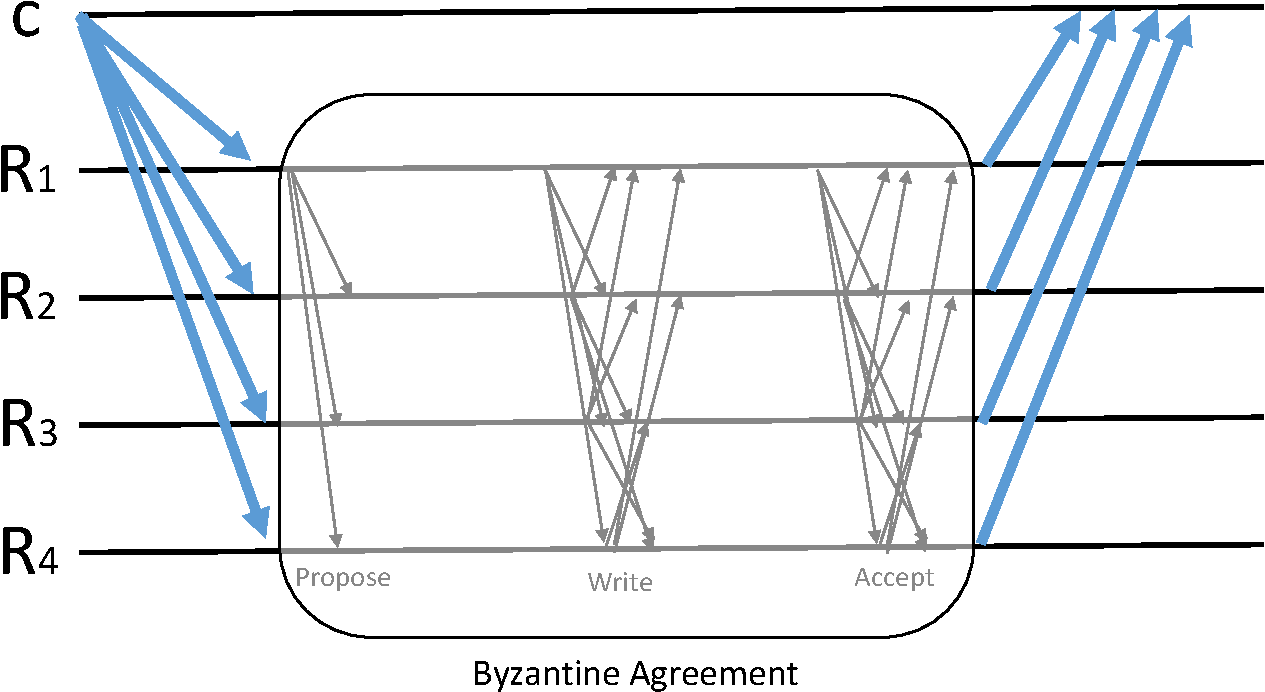
\includegraphics[width=.5\columnwidth]{images/images/bft.pdf}
\caption{Byzantine Fault Tolerance protocol overview.}
\label{fig:bft}
\end{center}
\end{figure}

Although \gls{bft} protocols provide safety to a bound of $f$ faulty nodes, with sufficient time $T$ an adversary eventually compromises $f+1$ nodes.
Then, additional mechanisms are needed to clean the faulty state (e.g., from time to time the nodes are recovered~\cite{Castro:2002}).
However, if a recovered node remains vulnerable to the same attack, the time to compromise $f+1$ becomes smaller as the attacker already knows how to exploit its vulnerabilities.
For this reason, several authors built their models assuming that the nodes fail independently due to some mechanism that provides failure independence (e.g.,~\cite{Castro:2002,Veronese:2013,Sousa:2010}).


\section{Byzantine Fault Tolerance}

Practical \gls{bft} replication was initially proposed as a solution to handle Byzantine faults of both accidental and malicious nature~\cite{Castro:1999}.
The correctness of a BFT service comes from the existence of a quorum of correct nodes, capable of reaching consensus on the (total) order of messages to be delivered to the replicas.
For instance, to tolerate a single replica failure, the system typically must have four replicas~\cite{Castro:2002,Kotla:2010,Aublin:2015}. 

Intrusion tolerance was first proposed by Fraga and Powell in 1985~\cite{Fraga:1985} as a solution to address faults without compromising the security of a system. 
Almost 15 years after, \gls{bft} replication became the most common solution to implement intrusion tolerance systems.
Castro and Liskov’s PBFT~\cite{Castro:1999} was the first practical \gls{bft} protocol. 
PBFT implements a \gls{smr} protocol that guarantees both liveness and safety for $\lfloor\frac{n-1}{3}\rfloor$ out of a total of n replicas. 
These properties hold even in asynchronous systems such as the internet. 
PBFT implements a SMR, therefore, it must guarantees that each replica executes the same commands, in the same order, and then it produces the same output. 
The protocol can be briefly described as follows: a client sends a message to all the replicas.
Then, the leader replica has to assign a sequence number to the request and multicast a pre-prepare message to the other replicas. 
If the replicas agree with the leader they send a prepare message to each other. 
At this phase of the protocol, every correct replica agrees on the ordering. 
A commit message is sent by every replica. When a replica receives the commit message from a quorum it executes the message. 
In the end, it replies to the client. 
Every replica shares a key with each other and with clients. These keys are used to authenticate messages with a \gls{mac}. 
The messages that are multicast by the clients are authenticated with a vector of \glspl{mac}. 
Then, each replica verifies its own \gls{mac}.
The authors implemented BFS, a Byzantine fault tolerant Filesystem, to validate this \gls{bft} library. 
The results show that when the workload increases the throughput and latency is nearly the same of a non-replicated system. 
This level of performance encouraged the use of \gls{bft} in common systems, and to develop optimizations to improve \gls{bft} protocols. 
Since the PBFT proposal, some work has been dedicated to improve \gls{bft} protocols (see Table~\ref{tab:bft}):


\begin{table}[h]
\begin{center}
{\footnotesize
\begin{tabular}{ p{2.5cm}  p{10.5cm}  }\hline
Zyzzyva~\cite{Kotla:2010}  & Introduces speculation to avoid the expensive three phase commit before processing the requests. This might introduce some inconsistency in the state of the replicas when speculation fails, and the client needs to help replicas to fix the servers’ inconsistency. \\ \hline			
Upright~\cite{Clement:2009} & It provides a straightforward way to also add BFT to crash fault tolerant systems (CFT); \\ \hline	
Aardvark~\cite{Clement:2009b} & Shifts the paradigm to a new design. This design improves the performance under faulty scenarios trading some performance on the normal case; \\ \hline
BFT-SMaRt~\cite{Bessani:2014} & It is modular and multicore-aware. Supports replica reconfiguration and has a flexible programming interface; \\ \hline
COP~\cite{Behl:2015} & It is the most recent BFT implementation that reached 2.4 million operations per second. This was achieved mostly due to BFT architecture changes.\\  \hline  
\end{tabular}
}
\caption{Brief overview of the most relevant BFT works.}
\label{tab:bft}
\end{center}
\end{table}

\paragraph{Summary.} 
Intrusion tolerance has an important role in our work, namely BFT-replication.
We propose a system that enhances intrusion tolerance by adding mechanisms that work on
top of a \gls{bft} replicated system. We need \gls{bft} protocols to guarantee that replicas execute in
the same order and to be able to tolerate some malicious failures in a subset of the replicas.
The implementation of such \gls{bft} protocol is a complex task, particularly if we need to
include mechanisms for state transfer, reconfiguration, and guarantee a good performance.
We prefer to rely on existent libraries than to build a new one.



\section{Replica Rejuvenation}


Software rejuvenation was proposed in the 90's~\cite{Huang:1993,Huang:1995} as a proactive approach to prevent performance degradation and failures due to software aging. 
The first proposals were based on periodical clean-up of the aging effects by restarting some parts of the software. 
This mechanism would postpone failures and restore the performance. 
This solution was implemented using three components: a watchdog process (\texttt{watchd}), a checkpointing library (\texttt{libft}) and a replication mechanism (\texttt{REPL}). 
A primary node executes the application while a backup node has the application inactive. 
The primary also runs the \texttt{watchd} to monitor the application crashes and hangs. 
In the backup, there is another watchdog watching the primary node. 
There is a routine (provided by \texttt{libft}) that periodically makes checkpoints and logging. 
These checkpoints are replicated with REPL in the backup node. 
When the primary node crashes or hangs, it is restarted, and if needed the backup takes his place on the execution.
PBFT-PR~\cite{Castro:2002} and COCA~\cite{Zhou:2002} introduced proactive recoveries in \gls{bft} replicated systems. 
Proactive Recovery is a mechanism that periodically rejuvenates the replicas to clean potential faults or stealth attacks. 
This mechanism allows that an adversary controls some replicas, usually $f$ , during a time window, where the system is vulnerable.
Castro and Liskov presented PBFT-PR~\cite{Castro:2002}, a BFT replication library that does proactive recovery (PR). 
PBFT-PR assumes that replicas will frequently recover. 
Additional assumptions are needed to guarantee the PBFT-PR's liveness and safety during the recoveries: 
(i) Each replica contains a trusted chip to store its private key, and it can sign and decrypt messages without revealing the key; 
(ii) The replicas’ public keys are stored in a BIOS read-only memory, which needs physical access to modify the BIOS; 
And last, (iii) a watchdog timer is used to avoid human interaction to restart replicas. 
The watchdog hands the execution to the recovery monitor, which cannot be interrupted.
Zhou~\etal{} presented COCA~\cite{Zhou:2002}, a fault-tolerant and secure online certification authority that has been built and deployed both in a local area network and on the internet.
COCA uses proactive signature sharing to ensure that when replicas fail and recover there
is no key-leakage. Contrary to PBFT-PR it does not rely on trusted components, but it may
need an administrator to refresh the COCA server keys.
Distler~\etal{} identified virtualization as a useful mechanism to implement proactive recovery in VM-FIT~\cite{Reiser:2007,Distler:2008}. 
The authors assume that an intrusion-tolerant replicated system executes in an untrusted domain, running in \gls{vm}. 
VM-FIT executes in a trusted domain, i.e., the \gls{vmm}. 
Virtualization allows the isolation between the untrusted and the trusted domains. 
Therefore, it can trigger recoveries from the trusted domain in a synchronous manner. 
Moreover, virtualization reduces downtime of the service during the recovery and makes the state transfer between replicas more efficient. 
The authors implemented this system using the Xen hypervisor to get the two domains: the trusted domain is the Xen Dom0, and the replicas run in the untrusted domains, DomUs.

Sousa~\etal{} improved the state-of-the-art recovery algorithms by introducing \gls{prrw}~\cite{Sousa:2010}. 
This technique removes the effects of faults ``immediately''. 
\gls{prrw} accelerates the rejuvenation process by detecting the faulty replicas behavior and forcing them to recover without sacrificing periodic rejuvenations. 
This type of technique can only be implemented with synchrony assumptions as the recoveries are time triggered~\cite{Sousa:2005}. 
To address this need the authors proposed an hybrid system model: the payload is an any-synchrony subsystem, and the wormhole is a synchronous subsystem. 
The authors implemented this system using the Xen hypervisor as the wormhole. 
Zhao~\etal{}~\cite{Zhao:2010} improved~\cite{Sousa:2010} with an algorithm to schedule the rejuvenations that is adaptable to a constant monitoring of the network and CPU/memory performance.

\paragraph{Summary.} \gls{bft} replication with proactive recovery represents one of the cornerstones of intrusion tolerance. 
PR allows the system to reduce the vulnerability window of the replicated system drastically. 
BFT replication with PR guarantees the system's correctness while the replicas recover faster than $f+1$ replicas become faulty. 
One limitation of PR is that there must be a trusted element somewhere to implement this mechanism. 
Some works use hardware timers while others resort to virtualization to separate the execution domains. 
In our proposal, we will adopt an architecture similar to~\cite{Distler:2008} and ~\cite{Sousa:2010}. 
However, our solution will implement a different (from~\cite{Sousa:2010}) algorithm to proactively trigger recoveries.


\section{Diversity}
\note{orgnize}
In some of the works presented before, the correctness is ensured under the assumption that replicas fail independently. 
Often the authors assume that fault independence is achieved using diversity~\cite{Castro:2002,Sousa:2010}. 
Diversity can be implemented in different ways~\cite{Deswarte:1998,Obelheiro:2006}, which may differ in the mean and the amount of diversity generated, but the goal is the same: to create different attack surfaces. 
The goal is to make the discovery of common vulnerabilities more difficult. 
We present at least three different ways to generate diversity: 
(i) N-version programming consists in design/implementation of different program binaries (from the same or different source code); 
(ii) Randomization implements different memory schemes; 
and (iii) Off-the-shelf diversity comprises the use of different products with the same functionality but taking advantage of implementations that are already available.

\note{citar survey \cite{Baudry:2015}}

\paragraph{N-version programming}
N-version programming is a technique used to create diverse software components~\cite{Randell:1975,Avizienis:1977,Avizienis:1985,Knight:1986,Chen:1995}.
The main idea behind this mechanism is to develop N different implementations of the same specification. 
These implementations can be implemented by N different developers or using translators to N different programming languages.

\paragraph{Artificial diversity.} 
Forrest~\cite{Forrest:1997} suggested randomized program transformations to introduce application diversity. 
They have made modifications on the gcc, a C compiler, in such a way that during the compiling time gcc inserts random padding
into each stack frame. 
%Linger presented stochastic diversification tool to swap code structures
The diverse versions are generated during the source code compilation. 
The main idea of these works is to make the intruder’s work more difficult when exploiting buffer overflow vulnerabilities.
Bhatkar~\etal{}~\cite{Bhatkar:2003} proposed a solution based on memory address obfuscation (i.e., \gls{aslr}). 
%Cox~\etal{}~\cite{Cox:2006} present N-variant system that uses automated diversity 
Their solution transforms object files and executables at the link-time and load-time, without kernel or compiler modifications. 
The goal is to ensure that an attack that succeeds in one target will not succeed on the other targets. 
Each time the program is executed its virtual addresses and data are randomized, and therefore the attacker needs to find new ways to exploit memory errors, like buffer overflows. 
However, a recent work proved that solutions like ASLR are vulnerable to attacks~\cite{Bittau:2014,Jang:2016}.
A few works propose the usage of compilers that generate different executables~\cite{Platania:2014,Roeder:2010,King:2016}.




\paragraph{Off-the-shelf diversity.}
The two previous solutions generate diversity before the software’s distribution. 
\gls{ots} diversity does not need pre-distribution of diverse mechanisms. 
It relies on the existence of different software components that are ready to be used.
There are plenty of different free products that provide the same functionality and were developed by different vendors. 
In other words, \gls{cots} diversity is like an opportunistic N-version programming.
Totel~\etal{} proposed an \gls{ids} based on design diversity~\cite{Totel:2005}.
The authors described an architecture that uses a set of replicated \gls{cots} servers, a proxy, and an \gls{ids}. 
The proxy is responsible for forwarding the requests from the client to every \gls{cots} server. 
When the servers reply, the proxy sends the responses to the \gls{ids} to be analyzed. 
The IDS compares the responses from the \gls{cots} servers and if it detects some differences an alarm is raised. 
Then the proxy votes the responses and replies to the clients. 
The authors developed an algorithm to detect intrusions and tested their solutions against Snort~\cite{snort} and WebStat~\cite{Vigna:2003}. 
The results show that using diverse-\gls{cots} service (e.g., http) allows the \gls{ids} to deliver fewer alarms without missing the intrusions.
Gashi~\etal{} made an experimental evaluation of the benefits of adopting diversity of SQL database servers~\cite{Gashi:2007}. 
The authors analyzed bug reports of four database servers (Post-greSQL, Interbase, Oracle, and Microsoft SQL Server) and verified which products were affected by each bug reported. 
They have found few cases of a single bug affecting more than one server. 
In fact, there were no coincident failures in more than two of the servers.
The conclusion is that \gls{ots} database servers’ diversity is an effective mean to improve system's reliability. 
However, the authors recognize the need for SQL translators, to increase the interoperability between servers in the replicated scenario.

Han~\etal{}. made a systematic analysis of the effectiveness of using \gls{ots} diversity to improve system's security~\cite{Han:2009}. 
First, the authors found if there were \gls{ots} software substitutes to provide the same functionality. 
Then, they determined if the \gls{ots} software shared the same vulnerabilities.
And if so, if the same vulnerability could be exploited with the same attack. 
In this study, more than 6k 1 vulnerabilities were analyzed, which were published in the \gls{nvd} on the year 2007. 
The results showed that 98.5$\%$ of the vulnerable software have substitutes. 
Moreover, the majority of them either did not had the same vulnerabilities or could not be compromised with the same exploit code. 
It is not expected that a single exploit works in different \glspl{os} because each one has a different memory scheme and different filesystems. 
Even between versions from the same \gls{os}, the low-level functions change across the versions. 
The study also concluded that 22.5$\%$ of the vulnerabilities were present in multiple software. 
However, only 7.1$\%$ from those vulnerabilities were present in software that offers the same service. 
The study findings are a good sign that diversity can improve a system’s dependability.
In a previous work, we studied \gls{ots} OSes diversity~\cite{Garcia:2014}. 
Similar to \cite{Han:2009} this study was carried out taking vulnerability feeds from \gls{nvd}. 
However, our work was only focused on OSes, and the data collected comprised 11-year of vulnerability reports. 
Our goal was to find to what extent different OSes shared common vulnerabilities. 
In this study, we analyzed 2270 vulnerabilities entries manually, where they were classified in different categories. 
Then, we defined three types of servers: (i) a server that contains most the packages/applications available (Fat server); (ii) a server that does not contain unnecessary applications to a certain
service (Thin server); and (iii) a thin server but with physically controlled access (Isolated hin server). 
We assumed that the third setting it is the most advisable for critical systems, since additional care is taken to install and setup its configuration. 
For each configuration, we compared all the common vulnerabilities in pairs of OSes. 
As expected, in the Isolated thin server, the number of common vulnerabilities was considerable less than in the other configurations. 
There was only 1 vulnerability that was shared among six OSes, 2 that were shared among five OSes, and 130 that are shared between two OSes. 
We went further in the study and looked for common vulnerabilities in different versions of the same OS. 
We have found evidence that suggests that using OS diversity in a replicated system can improve its dependability. 
Even if few OSes are employed, it is possible to achieve vulnerability independence just with different versions.



Larsen~\etal{} made a study with several examples on how to apply diversity~\cite{Larsen:2014,Larsen:2015}. 
The paper explains in detail what to diversify, from single instructions to an entire program. 
They also explain the three types of security impacts when diversity is applied: entropy analysis, attack-specific code analysis, and logical argument. 
However, they also point that there is no consensus on how to evaluate the efficacy of diversity. 


Zhai~\etal{}~\cite{Zhai:2014} propose a system that looks for independece failures from the reliability standpoint on the cloud.
The system collecs and audits data from the system components to evaluate its components' independence identifying potetianl correlated failures.
The authors collect information on networkd, hardware, and software data.
Then, the different configuration dependency are analyzed and ranked in risk groups as a way to see how the different dependencies may make the system fail.
The main limitation of this work is the motivation that clouds may not have to join such system, i.e., provide private data to be analyzed for extenral agents.
The experimental evaluation is concerned to the time that it takes to analyze all the data and creating the dependency graphs.
CITAR COM ESTE~\cite{George:2015}

EnvyFS -- reliability with N-version
Bairavasundaram and Sundararaman~\cite{Bairavasundaram:2009} implemented EnvyFS a filesystem that uses N-version filesystems implemenations to guarantee the reliability of stored data.
Their solution is able to tolerate filesystem mistakes (e.g., crash, integrity).
To keep the system simple, the authors used a virtual filesystem layer that abstract the specific filesystems underneeth, therefore some challenges arise from the differnet implementations details.
Another challenges, was to avoid the need for multiple storage as it uses N-variants of filesystems. 
However, they solved this by using the only one storage layer and the different filesystems in between. 
Then, after each filesystem executes the commands a voter collects the majority of outputs to store.
The results show that EnvyFS is able to improve the reliability by leveraging on multiple filesystems.
However, the performance results show that EnvyFS pays the price of executing in multiple filesystems and waiting for a majority of them. 
In most of the time it takes the sum of the three filesystems used.


%Network diversity 
Newell~\etal{} ~\cite{Newell:2015} presented a solution to assign diversity variants among network nodes to increase the network's resiliency (in particular its connectivity).
The authors present this as a Diversity Assignment Problem, although it is an NP-hard problem the authors show that for medium-size random networks graphs it is feasible.
For medium-sized networks they use mixed-integer programming and for larger networks propose a fast greedy approach.
For the first one the achieve optimality, and the latter an approximation of the optimal.
One of the results that the authors show is that random diversity assignment is far worse than an criteria assignment (as they propose).
Despite the different results that show improvements of diversity on the connectivity (i.e., resiliency), the models did not used realistic data, thus the authors assumed that the compromise values are known and independent with each other.


Zhang~\etal{}~\cite{Zhang:2016} propose a metric to evaluate the resilience of networks.
The idea is to define what is the least attacking effort to compromise some important assets of the networks (i.e., this work is focus on distributed yet not replicated systems).
Therefore, they measure the weakest path to target and compromise the main asset. 
The authors proposed three metrics which where evaluated in a simulated environment.
None of the three metrics uses vulnerability data to correlate the existence of common weakness, on contrary, the metrics use data about the topology, services installed, etc.
Nevertheless, the results show that increasing the diversity on the nodes reduces the number of simulated worms.
 

\paragraph{Summary.}
We presented three different techniques that support diversity as a fault-tolerant mechanism. 
N-version programming is the most costly, since it needs different developers or additional programs to verify if the automatic translation works. 
On the contrary, \gls{ots} and randomization diversity are almost for free. 
The first one can be obtained from free sources that are ready to be used, and the second one is automatic and already supported
in most OSes. 
Diversity still has some gaps that must be addressed to make it an effective building block of intrusion tolerance. 
For example, how to measure diversity in such a way that failure independence can be guaranteed?



\section{Vulnerability Analysis and Risk Management}

Bilge and Dumitras\cite{Bilge:2012} made a systematic study on zero-day attacks between 2008-2011.
In their study, the main dataset is \gls{wine} (developed by Symantec), it sample and aggreates data from several hosts running Symantec products (e.g., Norton Antivirus).
The \gls{wine} data is correlate with \gls{osvdb} and Symantec's Threat Explorer for attack/exploit information.
Their method allowed them to measre the duration of zero-day attacks, the average attack lasts ten months. 
Moreover, they have found that some of the vulnerabilities exploited during the Stuxnet attack have been employed two years before Stuxnet in another attack.
One of the main conclusions of this work is the evidence that the disclosure of zero-day vulnerabilities increases the risk, up to five orders of magnitude, of users being attacked.
The vendors are responsible to prioritize the disclosure of such vulneraiblities and prepare a patch as soon as possible. 

Nappa~\etal{}~\cite{Nappa:2015} analyzed the patch deployment process over 10 popular client applications on a 5-year period, in some cases, wich applications share libraries, the patching process takes different time to the same vulnerable shared code. 
The authors have found that there is a strong correlation between the vulnerability disclosed and the start patching process among vendors, for 77\% of the studied vulnerabilities it occuers within seven days. 
The performed a \emph{survival anylisis} (inspired in medice nad biology to measure the mortality rates associated with diseases) to measure the probability a vulnerable host will remain vulnerable beyond a specific time.
The vulnerability ''dies`` once a patch is installed or a non-vulnerable software is installed.
The experimental results show that using real-wordl WINE exploits still compromise 50\% of the vulnerable hosts (after vulnerabilties discloser). 
The median percentage of hosts that have been patched before the exploit is released is at most 14\%.
Together with the number of shared vulnerable code with different patching delays, these values motivate attackers to re-used already know exploits or to create patched-based exploits~\cite{Brumley:2008}.
The authors also show evidence to support the natural intuition that silent or automatic updades reduce the survivavility of vulnerabilties. 
They also, performed an analysis on three different user profiles that show that security analysts are more cureful on patching software than software developer or normal users.

Jumratjaroenvanit and Teng-amnuay~\cite{Jumratjaroenvanit:2008} described vulnerability life-cycles presenting their different stages. 
The authors goal was to understand how different dates can be useful to estimate the probability of an attack. 
The authors methodology was to collect and analyze data on the discovery, disclosure, and exploit dates, exploit and patch availability, all from public data sources. 
They used this information to define five life cycle types: (i) \gls{zda}, which typically is a done by a black-hat and is defined by the date of disclosure and exploit being the same; (ii) \gls{pzda}, is a \gls{zda} but with a patch already available, but not applied; 
(iii) \gls{ppzda}, is a \gls{pzda} but does not matter if the patch is available or not; 
(iv) \gls{poa}, it is a zero-day vulnerability. 
The most influential variables were the code that was scrutinized by a the tester with access to the source code, and the code that was analyzed with some static tool before. 
On the contrary, results showed that language safety was the less influent factor. 
The main result of the study was that two weeks of work were enough to have a 50\% chance of finding a zero-day vulnerability. 
Sometimes, 53 hours were enough to find one vulnerability with more than 95\% of probability.


Frei~\etal{}~\cite{Frei:2010} made a quantitive analysis of 27K vulnerabilities disclosed in the last decade.
The authors propose a model that describe the main players in a vulnerability lifecycle.
All the dates associated with the vulnerability lifecycle are described in details before the analysis.
They used a few public vulnerability databases (e.g., \gls{nvd} and \gls{osvdb}) to collect the different data attributes.
The results show that the number of patches increase after vulnerability disclosure.  
One interesting result is the \emph{the gap of insecurity} measurment, where they compare the patch availability vs the exploit availability. 
The results show that exploits are always ahead of patches, in some cases after 30 days of disclosure the number of exploits exceeds 90\% the number of patches.


Bozorgi~\etal{}~\cite{Bozorgi:2010} used machine learning techniques to classify existent vulnerabilites and predict future exploits.
Their results show that their trained classifiers outperform current exploitability measures like \gls{cvss} exploitability subscore.
They have built a dataset with two public databases Mitre' \gls{cve} (which is subpart of \gls{nvd}) and \gls{osvdb}.
They used the bag-of-words, a machine learning technique, to extact the textual attributes that are more relevant to analyse.
They used \gls{svm} to train the model, to conduct two types of experiments: an offline and an online.
In the offline setting, which they train and evaluate data in a static fashion, they achieve an accuracy of 90\% of correct predictions.
In the online settting, the results show that after a small period the model stablizes and reduces the overall error by 14\%.
In an online setting they were able to make preditions up to two days before the exploit with an accuracy of 75-80\%.
The main result, for the interest of this thesis, is the comparison between their model and the \gls{cvss} as a measure of indication of how a vulnreability is likely to be exploited.
The \gls{cvss} attributes high scores to vulnerabilities that were not exploited. 

Allodi and Massacci~\cite{Allodi:2014} made a in depth analysis of four security databases (e.g., \gls{nvd}, Exploit-DB, SYM, and EKITS). 
The authors made a in deph \emph{break down} of \gls{cvss} on its several attributes, for example, exploitability the subscore \emph{resembles more a constant than a variable}, thus not have a real impact on the \gls{cvss} score.
They used a randomized case-control study, which is applied to different study domains.
Is used to assess the effectiveness of a treatment over a sample of subjects.
In this study in particular the want to measure how \gls{cvss} influences the \emph{risk factor} of the studyie cases.
A result that is worth of note is that fixing vulnerabilities based on their \gls{cvss} is statistically equivalent to picking a random vulnerability to fix, from the security relevance standpoint.
On contrary, the authors suggest that it is more important to fix vulnerabilities that appear in the black market of vulnerabilities.
Their results indicate that the inclusion this information as a \emph{risk factor} can increase the risk redcution up to 80\%.
The authors point that EKITS datasource may be a threat to the validity of the study, as it is unstructured data and therefore it requires manually anaylsis.

Sabote~\etal{}~\cite{Sabottke:2015} presented a study that used non-common vulnerability data sources, i.e., Twitter data (e.g., specific words, the number of retweets, and replies, information about
the users posting these messages), to find exploit data. 
The authors made a quantitative and qualitative exploration of the vulnerability-related information disseminated on Twitter.
They developed a Twitter-based exploit detector to provide an adequate response in a such short time frame. 
This allows the security community to foresee the exploit activity before the information reaches the de facto disclosure data sources like \gls{nvd} and ExploitDB.
However, to complement and strength their information results they also used sources like \gls{nvd}, \gls{osvdb}, Exploit-DB, Microsoft Security Advisories and Symantec WINE. 
The authors distinguished the real-world exploits from the proof-of-concept exploits, as the latter are by products of the disclosure process. 
The real-world exploits typically are not known until a critical zero-day attack occurs. 
The authors used \gls{svm} to classify exploits in the social media and tested how robust it was to attacks, i.e., if a powerful attack could manipulate the information on Twitter with a false account and false data. 
The results showed that with their proposal they could be confident with the predictions. 
For example, the \gls{svm} classifier set to a precision of 25\% could detect the Heartbleed exploits within 10 minutes of its first appearance on Twitter. 
They also showed that organizations like \gls{nvd} overestimate the severity of some vulnerabilities that never become in fact exploited.
However, their work did not focus on the discovery of the zero-day vulnerabilities, which is relevant for our research.



Shahzad~\etal{}~\cite{Shahzad:2012} obtained data between 1988 to 2011 from three data sources: \gls{nvd}, \gls{osvdb}, and the data from~\cite{Frei:2006}. 
They collected vulnerabilities that affected popular applications like Internet Explorer, Firefox and Chrome, and popular \glspl{os} like Windows, Mac OS X, Solaris and several Linux distributions. 
The authors found that 2006 was the peak of vulnerability disclosures, and since then there was a decrease even though there are more software products. 
However, the complexity of the disclosed vulnerabilities has increased, ased on the \gls{cvss} score. 
From their dataset, 2.8\% vulnerabilities have an exploit released before their public disclosure. 
More dramatic is the percentage of exploits that are released on the day of the vulnerability disclosure, which is in the order of 88.2\%. 
There are a cases when even after the disclosure there are exploits being released (the authors found 9.7\% of their vulnerabilities fitting this condition). 
As already stated in~\cite{Gorbenko:2011}, the software’s popularity can be attractive to attackers. 
In this study, the authors found that Microsoft and Apple have more exploits before the vulnerability disclosure than the other vendors. 
This may primarily be because hackers find it more rewarding to exploit these products due to their wider market capitalization.
To what concerns patching, the authors argue that 10\% of the vulnerabilities had a patch before their disclosure, and 62\% had a patch on its disclosure day. 
There was a considerable number of vulnerabilities that were disclosed only after a patch is made, more precisely 28\%. 
However, the authors noticed that from 2007 there was an improvement from the vendors to respond to vulnerabilities with earlier patches. 
Nevertheless, the closed-source vendors are more efficient to patch vulnerabilities. 
Another conclusion is that it is easier to exploit opensource code vulnerabilities than in closed-source – this conclusion may seem obvious, but no one had showed it previously with statistical tests.


Holm~\cite{Holm:2014} made an analysis malware alarms to verify if there is a statistical distribution to model the number of intrusions or the time to compromise a computer system.
The author collected information from different software configurations from 2009 to 2012 from an IT enterprise.
The enterprise had a total of 697 \glspl{os} versions.
Each computer is equipped with an anti-malware software, when a malware is detected it sends the data to a central database.
The author's methodoly applied a few filters to reduce the size of the data by removing redudant information (e.g., a single malware can generate several alarms in the systems).
The results show that the Pareto distribution is the one that best fits for the time of the first compromise.
Another interesting result is that the more the system is intruded the more vulnerable it is. 
The authors present some hypothesis for this result, for example, once the system is broken it can no longer be trusted, but it seems odd to conclude something about how vulnerable the system is. 
A more plausible one is that the security awarness in only temporary increased as a result of the intrusion, and then it is again neglected.
Most of the malware considered in this study were not result of targeted attacks but rather automatic ones, this is probably due to the type of enterprise. 
This may change the results if applyied to targeted attacks as they require a different strategy to penetrate the system,.


%data analysis
Massacci and Nguyen~\cite{Massacci:2010} made an analysis of several datasources that provide data about vulnerabilities, exploits and patches. 
The authors raise some limitations on the datasources, namely the difficulty to map some of the listed sources. 
However, it is possible to use the \gls{nvd} mappings that provide code mappings for \gls{cve} and the respectevily ID from the other datasource.


%% MOVING TARGET ATTACKS

Okhravi~\etal{} presented TALENT a framework for live migration of critical infrastructures across heterogeneous platforms~\cite{Okhravi:2014,Okhravi:2009}. 
The idea was to create a moving target that difficult the success of advanced targeted attacks. 
TALENT implements OS level virtualization with containers, which allows the system to migrate the OS between machines periodically or upon detection of malicious activity. 
The virtualization was implemented with OpenVZ and LXC for Linux, Virtuozzo for Windows, and Jail for FreeBSD. 
The network was also virtualized, more precisely, a second layer of virtualization was used to migrate the IP address from one container to another. 
Even an established ssh session was preserved during the migration. 
Additionally, the state of the application also had to be migrated by employing a checkpointing technique. 
When all the programs were checkpointed, the state was saved and then was migrated by mirroring the filesystem. 
The filesystem synchronization took 98.7\% of the migration time. 
The authors decided to focus on optimizing the filesystem synchronization. 
In the optimized version, the filesystem synchronizes in periodic intervals by sending the differences to the destination. 
Therefore, the migration was made seamless to the application. 
TALENT also had a risk assessment, called operation assessment, which monitored and adjusted the diverse components using vulnerability information. 
However, there was almost no details on how the risk was measured and on how to adapt to the threats in an efficient manner.

Moving target \cite{Hong:2015}


Guo and Bhattacharya addressed the problem of \gls{bft} replicas fault independence~\cite{Guo:2014}.
The authors proposed different replicas configurations using OTS OSes to increase the diversity among the replicas. 
There was a set of different configurations that could build a replicated system. 
Each configuration was composed of different \gls{os}. 
The authors proposed a formalization of the virtual replica diversification problem. 
They used a game-theory approach to find an optimal diversification strategy for the defender's side. 
The authors validated their model with the \gls{nvd} data used in~\cite{Garcia:2012}.

Wang~\etal{} proposed a different approach to measure the risk~\cite{Wang:2014}. 
Contrary to the most common approaches that attempt to measure the vulnerability state of the syste, the authors explored how many zero-day vulnerabilities were required to compromise a network. 
They address diversity, however, as replication is not considered the use of diversity in a ''chained`` archictecture will no enhance the system's security.
One of the limitations of this approach is that it considers all zero day vulnerabilities equally likely to happen.
Moreover, the metric's calculatation is complex and no evaluation is provided to hint the reader on how long can it take to calculate.
A similar work is proposed in~\cite{Bopche:2015}.

%Similar to ours, but very weak.... need to read and show how it fails~\cite{Mu:2014}


Gorbenko~\etal{}~\cite{Gorbenko:2017} used \gls{cve} and \gls{nvd} databases to study vulnerability life-cycles of differnet \glspl{os}.
The authors made a particular effort to analyze the relation between vulnerabilities' discovery and their fix, more precisely the time it takes to vendors patch the vulnerable software.
Moreover, they also studied the existent of common vulnerabilities among different \glspl{os}.
The resuls of their study show between 2012 and 2016 most of \glspl{os} used in their study patched every vulnerability that was disclosed in that period, with the exception of Ubuntu Server 12.04.
Another interesting result are the results for \emph{forever-day vulnerability} (i.e., vulnerabilities that are publicly disclosed but not yeat patched). 
They show that, for the analyzed period, Ubuntu never had a single day free from vulnerabilities, and Windows and Red Hat had  only 12 and 10, respectevily.
However, the most important results is the implications of \gls{cvss} on the \emph{days-of-gray-risk} (i.e., the number of days it takes to a vendor releases a patch). 
The authors show that there is no obvious implication on the level of severity and the time it takes to a vendor develop a patch.


\paragraph{Summary.} We presented several works that carry out for risk assessment in a way to prevent exploits or to take action upon vulnerability detection. 
This is the last building block that intrusion tolerance is missing. 
There is a lot of relevant free information available to address the security and dependability of software. 
In a replicated context this information is even more relevant. 
First, to react upon vulnerability/exploit disclosures, and second to select what configurations are less vulnerable to common weakness. 
We want to explore the free available data to improve, the dependability and security of intrusion-tolerant systems, by ensuring the assumption of failure independence with evidence supported by  relevant data.
A few works in different goals than ours did analyze vulnerability textual data~\cite{Joshi:2013} -- citar mais tarde



\section{Pratical BFT Systems with Diversity}



(see ~\cite{Yuan:2014} for a survey)
SITAR~\cite{Wang:2003}

SCIT maybe the first one~\cite{Arsenault:2007}


In the last two decades there were a number of \gls{bft} protocols and systems deemed ``practical'' (e.g.,~\cite{Castro:2002,Kotla:2010,Veronese:2013,Aublin:2015,Behl:2015,Behl:2017,Liu:2016,Yin:2003}).
Most of these systems either ignore the issue of fault independence or simply assume it is solved in some way (e.g., N-version programming~\cite{Chen:1995} or \gls{ots} diversity~\cite{Gashi:2007,Garcia:2014}).
In principle, \system can support the execution of all these systems/protocols, as long as they support, or are extended to support, replica group reconfigurations, just like BFT-SMaRt~\cite{Bessani:2014}.
In this section, we discuss the few previous works that address the issue of diversity in \gls{bft} systems. 

BASE~\cite{Rodrigues:2001} is an extension of PBFT~\cite{Castro:1999} that explores opportunistic \gls{ots} diversity in \gls{bft} replication. 
The system provides an abstraction layer for running diverse service codebases on top of the PBFT library.
The key issue addressed by BASE is how to deal with different representations of the replica's state, allowing a replica that recovers from a failure to rebuild its state from other replicas. 
BASE was evaluated considering four different OSes and their native \gls{nfs} implementations: Linux, OpenBSD, Solaris, and FreeBSD.
The results, from 16 years ago, show the same trends we observed: performance varies significantly when diversity is considered.
Differently from \system, BASE does not address the selection of replicas or the reconfiguration of a replica group.

In order to support long-running services, Castro and Liskov~\cite{Castro:2002} introduced the notion of proactive recovery for \gls{bft} services. 
The objective is to rejuvenate replicas periodically to remove stealth attackers and support the execution of long-running services. 
All works on \emph{safe} proactive recovery consider the use of trusted local component on each replica to trigger the periodic recoveries~\cite{Castro:2002,Sousa:2010,Roeder:2010,Platania:2014,Distler:2011}.
%, and some of them even support reactive recoveries to deal with service degradations caused by detectable attacks~\cite{sousa:pc}.
A common weakness of most of these works is that they do not support diversity, therefore a compromised replica can be attacked immediately after its recovery by exploiting the same vulnerability.
The two noticeable exceptions are discussed in the following.

Roeder and Schneider~\cite{Roeder:2010} propose an intrusion tolerance technique called \gls{po} for supporting a different type of diversity from \system.
The idea is, instead of changing \glspl{os} or other off-the-shelf component of the replica, \gls{po} changes the application and library code periodically preserving the original semantics using program transformations, i.e., system call obfuscation reordering, memory randomization, and functions return checks (through an IBM \textit{gcc} patch that inserts and checks a random value after the functions return).
Each replica generates its own obfuscated executable from a read-only device containing the ``master code'' based on time-triggered epochs that a controller triggers in a secure way through a trusted component similar to \system' \gls{ltu}.
All obfuscation mechanisms were implemented and evaluated on OpenBSD 4.0, and their results show that PO adds a little extra overhead to the non-\gls{po} execution.

Similarly to \gls{po}, Platania~\etal{}~\cite{Platania:2014} proposed a compiler-based diversity for the Prime \gls{bft} protocol~\cite{Amir:2011} using the MultiCompiler tool~\cite{Homescu:2013}. 
This compiler creates diverse binaries from the same source code through randomization and padding techniques.
The authors also proposed a theoretical rejuvenation model that receives as input: the probability of a replica being correct over a year ($c$); the number of rejuvenations per day across the whole system ($r$); the number of replicas ($n$); and the system's lifetime. 
Although operators can control only $r$ and $n$, the authors suggest (but does not show how) that $c$ can be estimated using \gls{osint} from the internet (CERT alerts, bug reports, and other historical data).
The authors implemented their solution in two settings, including a virtualized environment provided by the Xen Hypervisor.
In this setting, each replica executes in a Linux \gls{vm}, the recovery watchdog runs in a trusted domain of the same machine, and the proactive-recovery controller runs in another physical machine, in an architecture similar to ours.


MOVNG TARGET HERE

\paragraph{Summary.} 
Diversity is becoming one of the building blocks of intrusion tolerance, alongside with \gls{bft} and rejuvenations. 
We presented few works that already used somehow diversity in intrusion-tolerant systems. Some of the works employed opportunistic \gls{ots} components to create diversity among the replicas. 
We do not discard the possibility of using other diversity techniques, such as randomization. 
However, in our work we are interested in \gls{ots} diversity because it is possible to estimate the vulnerability of each component. 
These works are still limited to that extent, i.e., there are none or few concerns on how to create diversity to avoid common failures. 
Most of the works implement diversity assuming complete fault independence, but that is unrealistic. 
For example, different \gls{ots} \glspl{os} can share the same weaknesses due to some shared libraries or kernel code. 
There is a need to understand how diversity can be efficiently employed in a replicated system to make the failure independence sound. 
Moreover, further work is still necessary to create automatic mechanisms that abstract diversity management for the administrators.

Both \gls{po} and the work from Platania~\etal{} improve the diversity of applications and replication libraries,\footnote{It should be noted, however, that recent studies have been shown that the benefits of these techniques are limited~\cite{Snow:2013,Bittau:2014}.} but not on \glspl{os} and other \gls{ots} components used by replicas.
Therefore, \system complements these services, as well as any proactive recovery system,\footnote{In particular, the ones that support proactive and reactive recoveries~\cite{Sousa:2010}.} by assessing and monitoring the potential risk of common-mode failures in a replicated service, and selecting appropriate replacements as the threat landscape evolves.

\system exploits the opportunistic \gls{ots} diversity derived from the existence of many version for \glspl{os}, \glspl{db}, Web Servers, \gls{jvm}, etc.
Several studies show that different versions of these components significantly increase chances of avoiding common-mode failures~\cite{Gashi:2007,Garcia:2014,Gorbenko:2011}.
Although we focus only on OSes in our \system prototype, the same techniques can be used to evaluate and deploy full diverse software stacks in the replicas.


\section{Final Remarks}







\chapter{A Study on Common Vulnerabilities}
\label{chap:datasource}

In this chapter we answer the following question: \emph{What are the security gains from using diverse \glspl{os} on a replicated intrusion-tolerant system?}
To answer this question, we have analyzed to what extent different \glspl{os} share common vulnerabilities.
We made an analysis using a well-established database and devise three strategies to build diverse sets of \glspl{os}.
The promising results confirm, to some extent, the intuition that diversity implies vulnerability independence.

\section{Methodology}

This section presents the methodology adopted in this study, with a particular focus on how the dataset was selected, processed and analyzed.

%\subsection{Object of the study}

\subsection{Data Source}
We have analyzed \gls{os} vulnerability data from the \gls{nvd} database~\cite{nvd}. 
According to \gls{nist} a vulnerability is defined as follows:
%\gls{nvd} uses the \gls{cve} definition of vulnerability \cite{cveterm}, which is given below:

\begin{defn}
 \emph{``[...] A weakness in an information system, system security procedures, internal controls, or implementation that could be exploited by a threat source.''}~\cite{Nist:2012}
\end{defn}


%\gls{nvd} aggregates vulnerability reports from more than 70 security companies, forums, advisory groups and organizations,\footnote{See the complete list on \url{http://cve.mitre.org/compatible/alerts_announcements.html}.} being thus the most complete vulnerability database on the web.
%All data is made available as \gls{xml} files containing the reported vulnerabilities on a given period, called \emph{data feeds}.

\gls{nist}'s \gls{nvd}~\cite{nvd} is the authoritative data source for disclosure of vulnerabilities and associated information~\cite{Massacci:2010}. 
\gls{nvd} aggregates vulnerability reports from more than 70 security companies, advisory groups, and organizations, thus being the most extensive vulnerability database on the web. 
All data is made available as \gls{xml} data feeds, containing the reported vulnerabilities on a given period. 
Each \gls{nvd} vulnerability receives a unique identifier, in the format CVE-\textit{YEAR}-\textit{NUMBER}, and a short description provided by the \gls{cve}~\cite{cveterm}. 
The \gls{cpe}~\cite{cpe} provides the list of products affected by the vulnerability and the date of the vulnerability publication.
The \gls{cvss}~\cite{cvss} calculates the vulnerability severity considering several attributes, such as the attack vector, privileges required, exploitability score, and the security properties compromised by the vulnerability (i.e., integrity, confidentiality, or availability).


We developed a program that collects, parses and inserts the \gls{xml} data feeds into an SQL database, deployed with a custom schema to group vulnerabilities by affected products and versions.

\subsection{Data Selection}
Despite the vast amount of information about each vulnerability available in \gls{nvd}, for this study, we are only interested in the name, publication date, summary (description), type of exploit (local or remote), and list of affected products.
We have collected vulnerabilities reported for 64 \gls{cpe}~\cite{cpe}.
Each one of these describes a system, i.e., a stack of software/hardware components in which the vulnerability may be exploited.
These \gls{cpe} were filtered, resulting in the following information that was stored in our database:

\begin{itemize}
\item \textbf{Part:} \gls{nvd} separates this in Hardware, \gls{os} and Application. For the purpose of this study we choose only enumerations marked as \gls{os};
\item \textbf{Product:} The product name of the platform;
\item \textbf{Vendor:} Name of the supplier or vendor of the product platform.
\end{itemize}


Those 64 CPEs were, by manual analysis, grouped in 11 \gls{os} distributions: \textit{OpenBSD, NetBSD, FreeBSD, OpenSolaris, Solaris, Debian, Ubuntu, Red Hat,\footnote{\textit{Red Hat} comprises the ``old'' Red Hat Linux (discontinued in 2003) and the newer Red Hat Enterprise Linux (RHEL).} Windows2000, Windows2003} and \textit{Windows2008}.
These distributions cover the most used \emph{\gls{os} products} of the BSD, Solaris, Linux and Windows families.

%We did not include Mac~OS~X because, unlike for the included OSes, we did not have an OS~X system available for cross-validation of vulnerability reports.

%\begin{figure}[!ht]
% \centering
% \includegraphics[width=0.9\columnwidth]{images/ea-crop.pdf}
% \caption{Simplified SQL schema of the database used to store and analyze the \gls{nvd} data. Fields not displayed are only used for auxiliary purposes.}
% \label{ea}
%\end{figure}

%The schema of the resulting database is displayed in Figure \ref{ea}.
%The tables with prefix \textit{cvss}, \textit{vulnerability\_type} and \textit{security\_protection} are employed to optimize the database.
%The most important tables are:

%\begin{itemize}
%\item \emph{cvss\_*} tables: refer directly to the Common Vulnerability Scoring System (CVSS) metrics \cite{cvss} of the stored vulnerabilities, which quantify the severity and impact of vulnerabilities;
%\item \emph{vulnerability}: stores basic data about a vulnerability (name, publication date, etc.) from the \gls{nvd} augmented with vulnerability life cycle information from the Open Source Vulnerability Database (OSVDB) \cite{osvdb};
%\item \emph{vulnerability\_type}: stores the vulnerability type assigned by us (see Section \ref{vulntypes});
%\item \emph{os}: stores the \glspl{os} platforms of interest in this study;
%\item \emph{os\_vuln}: stores the relationship between vulnerabilities and \glspl{os}, and their affected versions.
%\end{itemize}

The use of an SQL database brings at least three benefits when compared with analyzing the data directly from the \gls{xml} feeds.
First, it allows us to \emph{enrich the data set} by hand, for example, by associating release times and family names to each affected \gls{os} distribution.
Second, it allows us to modify the \gls{cve} fields to correct problems.
For instance, one of the problems with \gls{nvd} is that the same product is occasionally registered with distinct names in different entries;
For instance, (\textit{debian\_linux}, \textit{debian}) and (\textit{linux}, \textit{debian}) are two (product, vendor) pairs we have found for the Debian Linux distribution.
Other users of \gls{nvd} data feeds previously observed this same problem~\cite{cvedetails}.
Finally, an SQL database is much more convenient to work with than parsing the feeds on demand.

\subsection{Filtering the Data}\label{filtering_data}


From the more than 44,000 vulnerabilities published by \gls{nvd} at the time of this study, we selected 2563 vulnerabilities.
These vulnerabilities are the ones classified as \gls{os}-level vulnerabilities (``/o'' in their \gls{cpe}) for the \glspl{os} under consideration.

When manually inspecting the data set, we discovered and removed vulnerabilities that contained tags in their descriptions such as \emph{Unknown} and \emph{Unspecified}. 
These correspond to vulnerabilities for which \gls{nvd} does not know precisely where they occur or why they exist (however, they are usually included in the \gls{nvd} database because they were mentioned in some patch released by a vendor). 
We also found few vulnerabilities flagged as \emph{**DISPUTED**}, meaning that product vendors disagree that the vulnerability exists, and \emph{Duplicate}, used for vulnerabilities in which the \emph{summary} points to a duplicate entry or duplicate entry suspicion.
Due to the uncertainty that surrounds these vulnerabilities, we decided to exclude them from the study as well.

Table \ref{tab:unknowns} shows the distribution of these vulnerabilities across the analyzed \glspl{os}, together with the total number of valid vulnerabilities.

%TABLE 1
\begin{table}[!ht]
\begin{center}
{\scriptsize
\begin{tabular}{|l||c | c | c | c | c|}\hline
\textbf{OS} & \textbf{Valid} & \textbf{Unknown} & \textbf{Unspecified} & \textbf{Disputed} & \textbf{Duplicate}  \\\hline\hline % total
OpenBSD & 153 & 1 & 1 & 1 & 0 \\
NetBSD & 143 & 0 & 1 & 2 & 0  \\
FreeBSD & 279 & 0 & 0 & 2 & 0 \\
OpenSolaris & 31 & 0 & 52 & 0 & 0  \\
Solaris & 426 & 40 & 145 & 0 & 3  \\
Debian & 213 & 3 & 1 & 0 & 0  \\
Ubuntu & 90 & 2 & 1 & 0 & 0  \\
Red Hat & 444 & 13 & 8 & 1 & 1  \\
Windows2000 & 495 & 7 & 28 & 5 & 5  \\
Windows2003 & 56 & 5 & 34 & 3 & 5  \\
Windows2008 & 334 & 0 & 8 & 0 & 3   \\\hline\hline
\textbf{\#distinct vulns.} & 2270 & 63 & 210 & 8 & 12 \\ \hline
\end{tabular}
\caption{Distribution of OS vulnerabilities in NVD.}
\label{tab:unknowns}
}
\end{center}
\end{table}

An important observation about Table \ref{tab:unknowns} is that the columns do not add up to the number of distinct vulnerabilities (last row of the table) because some vulnerabilities are shared among \glspl{os} and are counted only once.
Notice that about 60\% of the removed vulnerabilities affected Solaris and OpenSolaris.
Moreover, these two systems are the only ones that have more than 10\% of its vulnerabilities removed.
We should remark that this manual filtering was necessary to increase the confidence that only valid vulnerabilities were used in the study.


\section{OS Diversity Study}\label{study}
This section analyzes the vulnerabilities that were shared in \gls{os} pairs over the period of 1994 to 2011. 
In the investigation, we consider two possible server machine setups offering an increasingly more secure platform. 
This accommodates the case where system administrators create differentiated \gls{os} installations, which contain more or less vulnerabilities depending on the services and applications available in the server. 
Of course, other setups could be used, but we decided to concentrate on these configurations because they are quite generic and they lead to results that can be directly obtained from the \gls{nvd} data. 
The setups are the following:

\begin{itemize}

\item \textbf{Fat Server:} The server contains most of the software packages for a given \gls{os}, and consequently, it can be used to run various kinds of applications by locally or remotely connected users. This server has potentially all vulnerabilities that were reported for the corresponding \gls{os};

%\item \textbf{Thin Server:} This setting corresponds to a platform that does not contain any applications (except for the replicated service). The server has a decreased security risk because the attack vectors related to applications have been mostly eliminated. 
%In this setting, vulnerabilities classified as \textit{Applications} are excluded from the statistics;

\item \textbf{Isolated Thin Server:} This setting corresponds to a platform that does not contain any applications (except for the replicated service). 
The server has a decreased security risk because the attack vectors related to applications have been mostly eliminated. 
Moroever, is placed in a room physically protected from illegal accesses, with remote logins disabled, and therefore it can only be compromised by receiving malicious packets from the network. In this setting, we only consider remotely exploitable vulnerabilities (those with ``Network'' or ``Adjacent Network'' values in their CVSS\_ACCESS\_VECTOR field) that are not classified as \textit{Applications}.

\end{itemize}

The Fat Server setup corresponds to a case where an attack may target an application available in the \gls{os} distribution. 
Therefore, it provides an upper bound estimate on the number of vulnerabilities that can be exploited. 
The Isolated Thin Server setups is the counterpart case, where the system is deployed without applications that come bundled with the \gls{os} and thus provide a lower bound estimate on the number of common vulnerabilities and it has the vulnerabilities that can be remotely exploited. 
Of course, in practice, at least one application (such as a name service or a distributed file service) would be deployed in an intrusion-tolerant system, and the vulnerabilities of this application would add up to the flaws that we will report. 
In any case, since we expect that most of the complexity is in the \gls{os}, we anticipate that a single application will have a small contribution to the overall number of vulnerabilities.



Intrusion-tolerant systems are usually built using four or more replicated servers~\cite{Castro:2002}. 
Therefore, it is useful to understand if there are many vulnerabilities that involve groups of \glspl{os} larger than two -- if this is the case, then it will be hard to find \gls{os} configurations for the various servers that do not share vulnerabilities, and a goal of using \gls{ots} diversity will be difficult to be achieved in practice. 
Figure \ref{top} portrays the number of common vulnerabilities that exist simultaneously in increasingly more extensive sets of \glspl{os} (with Isolated Thin Servers). 
The graph shows a rapid decrease in the shared vulnerabilities as the number of \glspl{os} grows. 
The largest group that was affected by the same vulnerability had six \glspl{os}, and this occurred only for a single flaw, and there were also two vulnerabilities in sets with five \glspl{os}. Vulnerabilities in two and three \glspl{os} usually occur in systems from the same family, whose common ancestry implies the reuse of more significant portions of the code base.
%As we have seen in previous tables, this is particularly true for the Windows and BSD families.

\begin{figure}[!h]
 \centering
 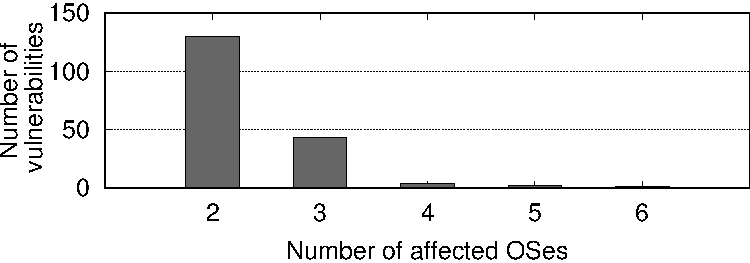
\includegraphics[]{images/gnuplot/spe/top/top.pdf}
 \caption{Common vulnerabilities for $n$ different OSes (with Isolated Thin Servers).}
 \label{top}
\end{figure}


Table \ref{tab:spreaded_vulns} lists in more detail the vulnerabilities that can be exploited in larger groups (four to six) of \glspl{os}. 
The first three bugs have a considerable impact because they allow a remote adversary to run arbitrary commands on the local system using a high-privilege account. 
They occurred either in widespread login services (telnet and rlogin) or in a primary system function, and consequently, several products from the BSD family were affected, as well as Solaris. 
The \gls{nvd} entry for the CVE-2001-0554 vulnerability also had external references to the Debian and Red Hat websites, which could indicate that these systems might suffer from a similar (or the same) problem. 
Vulnerability CVE-2008-1447 occurs in a large number of systems because it results from a bug in the BIND implementation of the \gls{dns}. Since BIND is a highly popular service, more \glspl{os} could potentially be affected. 
A closer look at the corresponding \gls{nvd} entry reveals external references to the sites of OpenBSD, NetBSD, and FreeBSD, indicating that they would be vulnerable in case this software was being used. 
This sort of vulnerability confirms that from an intrusion-tolerance perspective it is unwise to run the same server software everywhere, and that diverse implementations must be selected (in this case for recursive \gls{dns} servers).


\begin{table}[!ht]
\begin{center}
{\scriptsize
\begin{tabular}{|c||c| p{7,8cm} | }\hline
\textbf{CVE} & \#affected OS  & Description  \\\hline\hline
CVE-1999-0046  &  4  & Buffer Overflow of \emph{rlogin} allows admin access. Affects: NetBSD, FreeBSD, Solaris and Debian. \\ \hline
CVE-2001-0554  &  4  & Buffer overflow in telnetd (telnet daemon) allows remote attackers to execute arbitrary commands. Affects: OpenBSD, NetBSD, FreeBSD and Solaris.  \\ \hline
CVE-2003-0466  &  4  & Off-by-one error in the Kernel function \emph{fb\_realpath()} allows admin access. Affects: OpenBSD, NetBSD, FreeBSD and Solaris.  \\ \hline
CVE-2005-0356  &  4  & TCP implementations allow a denial of service (DoS) via spoofed packets with large timer values, when used with Protection Against Wrapped Sequence Numbers. Affects: OpenBSD, FreeBSD, Windows2000 and Windows2003. \\ \hline
CVE-2008-1447  &  5  & The BIND 8 and 9 implementation of the DNS protocol allow attackers to spoof DNS traffic via a birthday attack to conduct cache poisoning against recursive resolvers. Affects: Debian, Ubuntu, Red Hat, Windows2000 and Windows2003.  \\ \hline
CVE-2001-1244  &  5  & TCP implementations allow a DoS by setting a maximum segment size very small to force the generation of more packets, amplifying network traffic and CPU consumption. Affects: OpenBSD, NetBSD, FreeBSD, Solaris and Windows2000. \\ \hline
CVE-2008-4609  &  6  & TCP implementation allows a DoS via multiple vectors that manipulate TCP state table. Affects: OpenBSD, NetBSD, FreeBSD, Windows2000, Windows2003 and Windows2008.   \\ \hline
\end{tabular}
}
\caption{Vulnerabilities that affect more than four OSes.}
\label{tab:spreaded_vulns}
\end{center}
\end{table}


The remaining three vulnerabilities are related to the TCP/IP protocol stack. 
All of them affect system availability, allowing different forms of \gls{dos} attacks. 
CVE-2008-4609 is the vulnerability that affects more \glspl{os}, according to the \gls{nvd} database. 
Given that TCP/IP stack code is often reused across \glspl{os}, we checked the websites of the other \glspl{os} for reports related to this vulnerability. 
We only found a disclaimer by Red Hat~\footnote{\url{https://access.redhat.com/kb/docs/DOC-18730}} stating that this flaw affected some releases but that they would not provide an update (they only offered a mitigation solution based on IPtables, the Linux firewall software).

Overall, the above results look encouraging because over a significant period (around 18 years) there are very few vulnerabilities that appear in many \glspl{os}. 
A good portion of them are in the TCP/IP stack implementation, which is probably the most shared software component across \glspl{os}, but they only impact on the availability of the system, leaving confidentiality and integrity of data unharmed.


\section{Strategies for OS Diversity Selection}\label{evaluation}
The prelimary analysis indicate that it is possible to find that some \glspl{os} share less vulnerabilities than others. 
Therefore, in this section we present three alternative strategies to select \glspl{os}, based on the built dataset, to decrease the chance of common vulnerabilities on replicated systems. 
We start the section by first describing an approach we called the \gls{cvi}, which is used by one of the strategies. 
For each strategy, we then give example sets of \glspl{os} that exhibit a reasonable level of diversity, and perform an evaluation based on the collected data. 
Finally, we conclude the section with an analysis of potential diversity between releases of the same \glspl{os} (concentrating on the \glspl{os} that the three strategies picked as the best configuration).


\subsection{Common Vulnerability Indicator}\label{cvi}
In a previous work~\cite{Garcia:2012} we have found that the number of common vulnerabilities that are observed between different \glspl{os} varies over time. 
Thus, in order to be able to evaluate which \gls{os} pairs are more (or less) likely to experience common flaws while taking into account the timing of vulnerability disclosures, we developed a new metric, called the \emph{\gls{cvi}}. 
This indicator is calculated for a given year $y$, based on the vulnerabilities that were shared by \glspl{os} A and B over a period of $\mathit{tspan}$ previous years. \gls{cvi} is built to ensure the following desirable properties:
\begin{enumerate}
\newcommand{\OLDtheenumi}{\theenumi}
\renewcommand{\theenumi}{\roman{enumi}}
\item $\mathit{CVI}_y(A,B) = 0$ if A and B have no common vulnerabilities in the $\mathit{tspan}$ interval;
\item $\mathit{CVI}_y(A,B) < \mathit{CVI}_y(C,D)$ if A and B shared less vulnerabilities than C and D in each year of the considered period;
\item $\mathit{CVI}_y(A,B) < \mathit{CVI}_y(C,D)$ if A and B had $N$ common vulnerabilities in the distant past while C and D had $N$ shared vulnerabilities more recently;
\item $\mathit{CVI}_{y_2}(A,B) < \mathit{CVI}_{y_1}(A,B)$, with $y_1 < y_2$, if the number of common vulnerabilities for A and B has decreased over the years.
\renewcommand{\theenumi}{\OLDtheenumi}
\end{enumerate}

Therefore, \gls{cvi} is useful for comparison purposes, allowing the identification of \gls{os} pairs that have a smaller number of common flaws, while considering the instant when vulnerabilities were found. 
This last point is particularly crucial because \glspl{os} are continually evolving, potentially getting more (or less) diverse, and consequently, one should take into consideration the time dimension when selecting \gls{os} configurations (e.g., \gls{os} pairs that have had less common flaws recently are likely better candidates).
\gls{cvi} is computed as follows:

First, a weighting factor $\alpha_{i}$ is defined for each year   $i \in \{y-\mathit{tspan}+1, ..., y-2, y-1, y\}$.

\begin{equation}
\alpha_{i} = 1 - \frac{y-i}{\mathit{tspan}}
\end{equation}

Then, CVI is obtained using the number of vulnerabilities $v_{i}(A,B)$ that appeared in both \glspl{os} A and B for every year $i$ from the start of the time span up to reference year $y$.

\begin{equation}
\mathit{CVI}_{y}(A,B)= \sum_{i = y-\mathit{tspan}+1}^{y} \alpha_{i}\cdot v_{i}(A,B)
\end{equation}


\begin{table}[!ht]
\begin{center}
{\scriptsize
\begin{tabular}{|l|c c c|| c c c |}
\cline{2-7}
\multicolumn{1}{c}{} &  \multicolumn{3}{|c||}{\textbf{Fat Server}}  &  \multicolumn{3}{|c|}{\textbf{Isolated Thin Server}} \\ \hline
OS             & 2009 &	2010 & 	2011        & 	2009 & 	2010 & 2011 \\ \hline
OpenBSD-NetBSD  & 17.1 & 13.8 & 14.8        & 8.4 & 7.1 & 6.9   \\
OpenBSD-FreeBSD & 22.2 & 18.0 & 18.1        & 14.1  & 11.6 & 10.3  \\
OpenBSD-Solaris & 4.0 & 3.1 & 3.3           &  1.8 & 1.4 & 0.9  \\
OpenBSD-Debian  & 1.7 & 1.5 & 1.4           &  0.0 & 0.0 & 0.0  \\
OpenBSD-Red Hat & 5.0 & 4.1 & 3.2           &  1.6 & 1.4 & 1.1  \\
OpenBSD-Win2000 & 1.8 & 1.5 & -             &  1.8 & 1.5 & -  \\  \hline
NetBSD-FreeBSD  & 19.7 & 18.3 & 18.8        & 11.0 & 9.3 & 8.6 \\
NetBSD-Solaris  & 4.9 & 4.0 & 4.2           &  1.5 & 1.1 & 0.7  \\
NetBSD-Debian   & 1.4 & 0.9 & 0.5           &  0.6 & 0.4 & 0.2  \\
NetBSD-Red Hat  & 1.8 & 1.1 & 0.5           &  0.6 & 0.4 & 0.2  \\
NetBSD-Win2000  & 1.6 & 1.4 & -             & 1.6 & 1.4 & -   \\ \hline
FreeBSD-Solaris & 6.5 & 5.4 & 6.3           & 2.3 & 1.7 & 1.2  \\
FreeBSD-Debian  & 1.3 & 0.8 & 0.5           & 0.0 & 0.0 & 0.0  \\
FreeBSD-Red Hat & 5.6 & 4.4 & 3.3           & 1.7 & 1.4 & 1.1  \\
FreeBSD-Win2000 & 2.3 & 1.9 & -             & 2.3 & 1.9 & -  \\ \hline
Solaris-Debian  & 1.0 & 0.8 & 0.6           & 0.0 & 0.0 & 0.0  \\
Solaris-Red Hat & 5.3 & 6.5 & 5.5           & 1.0 & 0.7 & 0.5  \\
Solaris-Win2000 & 5.5 & 5.7 & -             & 1.0 & 0.7 & -  \\ \hline
Debian-Red Hat  & 26.1 & 20.5 & 15.7        & 3.2 & 2.1 & 1.4  \\
Debian-Win2000  & 0.9 & 0.8 & -             & 0.9 & 0.8 & -   \\ \hline
Red Hat-Win2000 & 1.8 & 1.6 & -             & 0.9 & 0.8 & -   \\ \hline
\end{tabular}
\caption{CVI for the years 2009 to 2011, with $\mathit{tspan}$ of 10 years.}
\label{tab:cvi-2011-2009}
}
\end{center}
\end{table}

Table~\ref{tab:cvi-2011-2009} presents \gls{cvi} values for the years 2009 to 2011. 
We have excluded from this analysis \glspl{os} with vulnerability information missing for more than one year over the period, to avoid using incomplete data in the calculation of the indicators. Therefore, the following \glspl{os} were not considered in Table~\ref{tab:cvi-2011-2009}: Windows2003, Windows2008, Ubuntu, and OpenSolaris. 
The \gls{cvi} values are computed for a $\mathit{tspan}$ of 10 years to reflect a reasonable history. 
It is possible to see that, except for one system (Solaris with FreeBSD/Red Hat/Windows2000 in the Fat Server), in all remaining cases \gls{cvi} shows a decreasing trend. 
Several of the \glspl{os} that have evolved over a considerable period are having less reported vulnerabilities, and this causes a decline in shared vulnerabilities in the recent years. 
For some of the \gls{os} pairs the drop in the \gls{cvi} value is quite significant, becoming almost one-third of the 2009 value (NetBSD with Debian or Red Hat). 
In the Isolated Thin Server case, there are three pairs with $\mathit{CVI}(A,B)=0$, which shows that they have shared no vulnerabilities during the past 12 years, and are thus particularly good candidates to include in intrusion-tolerant configurations. 
These systems are Debian with either OpenBSD or FreeBSD or Solaris.

%According to Table~\ref{tab:pairs_vulns_by_year}, both \gls{os} pairs had 10 common vulnerabilities in the 2000--2011 period, suggesting that they both provide the same degree of diversity. 
From the \gls{cvi} values in Table~\ref{tab:cvi-2011-2009}, it is apparent that OpenBSD and Red Hat have become more diverse, in recent years, than Red Hat and Solaris, and to make it advisable, from a diversity standpoint, to choose the former \gls{os} pair over the latter.



\subsection{Building Replicated Systems with Diversity}
\label{build_diversity}


This section describes three strategies for choosing diverse sets of \glspl{os}. 
These strategies utilize the data analyzed earlier as a basis to make decisions, by assuming that the information reported by \gls{nvd} on vulnerabilities can be correlated to the amount of diversity among \glspl{os}. 
Of course, there are some caveats associated with this approach, but the alternatives can be even harder to put in practice, especially if one wants to consider a large number of \glspl{os}. 
For example, for closed systems (e.g., Windows) it is challenging to determine the level of sharing of \gls{os} components, and therefore, diversity estimations based on the code cannot be performed. Moreover, even if this estimate could be obtained, there is the risk that it does not reflect the number of vulnerabilities that occur simultaneously in several \glspl{os} (e.g., two distinct implementations of the same flawed algorithm are vulnerable).

The first strategy, called \gls{cvcs}, is based on raw data collected over a considerable interval, and is the most straightforward approach for selecting \gls{os} pairs. 
It should be used when one wants to treat all vulnerabilities, regardless of the time which they were reported, as equally important to make choices. 
The second strategy, \gls{cvis}, uses the \gls{cvi} described in the previous section to select \gls{os} pairs taking into account the incidence of common vulnerabilities over the years. 
It is indicated when one wants to give greater importance to more recent vulnerabilities because it is a weighted sum. 
The third strategy, \gls{irts}, follows a different approach from the previous ones, focusing not so much on common vulnerabilities directly, but on the frequency in which vulnerabilities appear in the two OSes. If one wants to give more importance to the time interval between successive reports of common vulnerabilities, this is the best strategy. 
Since this last criterion complements the previous two, one could explore strategies \gls{cvcs} and \gls{cvis} in conjunction with \gls{irts}.

For every strategy, we present example \gls{os} sets for the Fat Server and Isolated Thin Server configurations. 
Fat Server configurations can be pessimistic in the sense that they may account for common vulnerabilities in applications that are not present in the servers, while Isolated Thin Server configurations reflect more accurately the expected setup of dedicated servers in a replicated system. 
An intrusion-tolerant system usually requires $3f+1$ replicas to tolerate $f$ intrusions (e.g., \cite{Castro:2002}). 
Therefore, we will focus on sets with four \glspl{os} to deploy a hypothetical replicated system with four replicas, which allows one fault to be tolerated.

As a cautious note, one should take into account that Ubuntu and Windows2008 were first released in 2004 and 2008 respectively, so the data for these two \glspl{os} was collected for a smaller number of years. 
Windows2000 is presented in the tables because there are published vulnerabilities until 2010, although it has been gradually replaced by Windows2003 and Windows2008 in the organizations. Consequently, we do not use Windows2000 when choosing the \gls{os} sets. 
We have excluded OpenSolaris from the study because there is data available for only a limited period. 
In each strategy and configuration we present two sets: \emph{setCon} is more conservative, since it does not contain Ubuntu and Windows2008; and \emph{setUpdt} is more up-to-date because it can include Ubuntu and Windows2008. 
When looking at these two sets, one should keep in mind that setCon is selected from a group of \glspl{os} for which there is a significant amount of \gls{nvd} data, which contributes for higher confidence on the result. 
On the other hand, setUpdt uses \glspl{os} with different amounts of \gls{nvd} data, which can cause small levels of inaccuracy when making comparisons (e.g., in the \gls{cvcs}, any \gls{os} pair featuring Windows2008 has zero common vulnerabilities until 2007). 
One way to address this would be only to consider vulnerabilities that appear later than 2007 when choosing setUpdt. 
We opted not to follow this approach because it has the drawback of discarding too much data.


\subsection{Common Vulnerability Count (CVCst)} 

The results from the previous section give a strong indication that it should be possible to choose groups of \glspl{os} with few common vulnerabilities over reasonable intervals of time. 
However, we would like to understand if the data from the \gls{nvd} database is effective at suggesting these groups of \glspl{os}. 
To address this point, we divided the data into two subsets: the \emph{history period}, comprising the data for the interval between 2000 to 2009, and the \emph{observed period}, from 2010 to 2011. 
The objective is to employ the historical period to pick the sets of \glspl{os} to use on the replicated system (as if the choice was made at the beginning of 2010). Then we use the data for the observed period to verify if these choices would have been adequate, i.e., if they have a small (preferably the smallest) number of common vulnerabilities in this period.

\gls{cvcs} makes decisions based directly on the empirical data for the number of common vulnerabilities across all \gls{os} pairs. 
This data is displayed in Table \ref{tab:strat_i} for \glspl{os} with a Fat Server configuration. 
Numbers to the right and above the diagonal line represent the history period, while numbers to the left and below the line stand for the observed period. 
For example, the entry corresponding to OpenBSD-Red Hat to the right of the diagonal line has the number 10, which means that these \glspl{os} shared 10 vulnerabilities between 2000 and 2009. 
The equivalent entry, but to the left of the diagonal line, is 0 because they had no common flaws reported in 2010 and 2011. 
As expected, \gls{os} pairs from the same family had the highest counts of common vulnerabilities. 
The only case where there were more vulnerabilities in the observed period than the historical period is for the Windows2008--Windows2003 pair, which is explained by the recent release date of Windows2008. 
It is interesting to notice, however, that most pairs had zero common vulnerabilities in the observed period.


\begin{table}[!ht]
\begin{center}
{\footnotesize
\begin{tabular}{|l|c|c|c|c|c|c|c|c|c|c|c|c|}\cline{2-11}
 \multicolumn{1}{c|}{} &
\begin{sideways}\vspace{2mm}\parbox{2mm}OpenBSD\end{sideways}&
\begin{sideways}\vspace{2mm}\parbox{2mm}NetBSD\end{sideways}&
\begin{sideways}\vspace{2mm}\parbox{2mm}FreeBSD\end{sideways}&
\begin{sideways}\vspace{2mm}\parbox{2mm}Solaris  \end{sideways}&
\begin{sideways}\vspace{2mm}\parbox{2mm}Debian\end{sideways}&
\begin{sideways}\vspace{2mm}\parbox{2mm}Ubuntu \end{sideways}&
\begin{sideways}\vspace{2mm}\parbox{2mm}Red Hat\end{sideways}&
\begin{sideways}\vspace{2mm}\parbox{3mm}Win2000 \end{sideways}&
\begin{sideways}\vspace{2mm}\parbox{3mm}Win2003 \end{sideways}&
\begin{sideways}\vspace{2mm}\parbox{3mm}Win2008  \end{sideways}&
\multicolumn{2}{|c}{} \\ \cline{1-11}  \cline{1-12}
OpenBSD & - & 33 & 43 & 9 & 2 & 3 & 10 & 3 & 2 & 1&   \multirow{13}{1mm}{\begin{sideways}\hspace{8mm}\parbox{15mm}{2000-2009}\end{sideways}} \\ \cline{1-11}
NetBSD & 4 & - & 36 & 9 & 4 & 0 & 6 & 3 & 2 & 1  &\\ \cline{1-11}
FreeBSD & 4 & 6 & - & 12 & 4 & 2 & 12 & 4 & 3 & 1& \\ \cline{1-11}
Solaris & 1 & 1 & 2 & - & 2 & 2 & 8 & 8 & 7 & 0 &\\ \cline{1-11}
Debian & 0 & 0 & 0 & 0 & - & 14 & 52 & 1 & 1 & 0 &\\ \cline{1-11}
Ubuntu & 0 & 0 & 0 & 0 & 0 & - & 27 & 1 & 1 & 0 &\\ \cline{1-11}
Red Hat & 0 & 0 & 0 & 2 & 0 & 0 & - & 2 & 2 & 0 &\\ \cline{1-11}
Win2000 & 0 & 0 & 0 & 1 & 0 & 0 & 0 & - & 216 & 42 &\\ \cline{1-11}
Win2003 & 0 & 0 & 0 & 1 & 0 & 0 & 0 & 49 & - & 53 & \\ \cline{1-12}
Win2008 & 0 & 0 & 0 & 1 & 0 & 0 & 0 & 38 & 229 & -	& \multicolumn{1}{|c}{}  \\ \cline{1-11}
 \multicolumn{1}{c|}{}& \multicolumn{9}{|c|}{2010-2011} & \multicolumn{2}{|c}{}\\ \cline{2-10}
\end{tabular}
\caption{History/observed period for CVCst with Fat Servers.}
\label{tab:strat_i}
}
\end{center}
\end{table}


The strategy for building sets of \glspl{os} is based on a simple cost function. 
Given any potential \gls{os} pair A and B that could be added to the set, one can perform a lookup in Table \ref{tab:strat_i} to determine the pair's number of common vulnerabilities in the historical period. 
This number corresponds to the cost of adding this \gls{os} pair to the group. 
Similarly, when including a third \gls{os} C, it is possible to find in the table the entries for A--C and B--C and take their sum as the cost of integrating C in the group. 
When building a set with $n$ \glspl{os}, the total cost is the addition of each individual cost for all combinations of \gls{os} pairs.
The sets that lead to smaller values of total cost are considered the best choices for deployment in the replicated system.
Accordingly, based on the table, the best groups of four \glspl{os} are:

\begin{itemize}
  \setlength\itemsep{0em}
\item setCon = \{\emph{OpenBSD, Solaris, Debian, Windows2003}\}, with a total cost of 23;
\item setUpdt = \{\emph{NetBSD, Solaris, Ubuntu, Windows2008}\}, with a total cost of 12.%, but one vulnerability affects more than two \glspl{os} simultaneously, hence two pairs.
\end{itemize}


One, however, should keep in mind that sometimes the total cost may be only an approximation of the actual number of shared vulnerabilities among the \glspl{os} in the set, as specific vulnerabilities might be counted more than once. 
This will likely not be a problem since overcounting vulnerabilities provides a conservative estimate, or an estimate worse than reality. 
For example, setUpdt only has 11 shared vulnerabilities for a total cost of 12, since one of the vulnerabilities appears in three of the \glspl{os} (and is therefore included in two table entries).

Next we can check to what extent our choice of the best group of four \glspl{os} that we would pick from the historical period (2000--2009), as prescribed by \gls{cvc} cost calculation, remains consistent with the choice of the best group of four \glspl{os} from the observed period (2010--2011). 
We see that both setCon and setUpdt have only two shared vulnerabilities. 
They are not the best sets in the observed period (2010--2011), since there are groups of \glspl{os} with zero common vulnerabilities in the observed period (e.g., by replacing Solaris with Red Hat), though they do exhibit a high level of diversity. 
A graphical representation of the sets as Venn diagrams is available in Figures~\ref{fig-venn}(a) and~\ref{fig-venn}(b). 
Below the \gls{os} name is the total number of vulnerabilities during the observed period, and the number inside each intersection shows the count of common flaws for the corresponding \glspl{os}. 
For example, in setCon with Fat Servers (Figure~\ref{fig-venn}(a)) there is one vulnerability that appears both on Solaris and OpenBSD and another on Solaris and Windows2003.


\begin{table}[!ht]
\begin{center}
{\footnotesize
\begin{tabular}{|l|c|c|c|c|c|c|c|c|c|c|c|c|}\cline{2-11}
 \multicolumn{1}{c|}{} &
\begin{sideways}\vspace{2mm}\parbox{2mm}OpenBSD\end{sideways}&
\begin{sideways}\vspace{2mm}\parbox{2mm}NetBSD\end{sideways}&
\begin{sideways}\vspace{2mm}\parbox{2mm}FreeBSD\end{sideways}&
\begin{sideways}\vspace{2mm}\parbox{2mm}Solaris  \end{sideways}&
\begin{sideways}\vspace{2mm}\parbox{2mm}Debian\end{sideways}&
\begin{sideways}\vspace{2mm}\parbox{2mm}Ubuntu \end{sideways}&
\begin{sideways}\vspace{2mm}\parbox{2mm}Red Hat\end{sideways}&
\begin{sideways}\vspace{2mm}\parbox{3mm}Win2000 \end{sideways}&
\begin{sideways}\vspace{2mm}\parbox{3mm}Win2003 \end{sideways}&
\begin{sideways}\vspace{2mm}\parbox{3mm}Win2008  \end{sideways}&
\multicolumn{2}{|c}{} \\ \cline{1-11}  \cline{1-12}
OpenBSD & - & 13 & 26 & 5 & 0 & 0 & 3 & 3 & 3 & 1&\multirow{13}{1mm}{\begin{sideways}\hspace{8mm}\parbox{15mm}{2000-2009}\end{sideways}} \\ \cline{1-11}
NetBSD & 1 & - & 18 & 4 & 2 & 0 & 2 & 3 & 1 & 1& \\ \cline{1-11}
FreeBSD & 1 & 1 & - & 6 & 0 & 0 & 3 & 4 & 2 & 1& \\ \cline{1-11}
Solaris & 0 & 0 & 0 & - & 0 & 0 & 2 & 2 & 1 & 0& \\ \cline{1-11}
Debian & 0 & 0 & 0 & 0 & - & 2 & 8 & 1 & 1 & 0 &\\ \cline{1-11}
Ubuntu & 0 & 0 & 0 & 0 & 0 & - & 1 & 1 & 1 & 0 &\\ \cline{1-11}
Red Hat & 0 & 0 & 0 & 0 & 0 & 0 & - & 1 & 1 & 0 &\\ \cline{1-11}
Win2000 & 0 & 0 & 0 & 0 & 0 & 0 & 0 & - & 81 & 13 &\\ \cline{1-11}
Win2003 & 0 & 0 & 0 & 0 & 0 & 0 & 0 & 4 & - & 14 &\\ \cline{1-12}
Win2008 & 0 & 0 & 0 & 0 & 0 & 0 & 0 & 3 & 26 & - & \multicolumn{1}{|c}{}  \\ \cline{1-11}
 \multicolumn{1}{c|}{}& \multicolumn{9}{|c|}{2010-2011} & \multicolumn{2}{|c}{}\\ \cline{2-10}
\end{tabular}
\caption{History/observed period for strategy CVCst with Isolated Thin Servers.}
\label{tab:strat_i_iso}
}
\end{center}
\end{table}


Table \ref{tab:strat_i_iso} presents the common vulnerabilities with the Isolated Thin Server configuration data. This configuration represents a class of servers that have a dedicated function and are protected against physical intruders. 
The same approach can be applied as above: first, we choose the best pairs based on the historical period to build a set of four \glspl{os}; next, we evaluate the sets by comparing the results with the values for the observed period. 
The history period provides two candidate sets: 

\begin{itemize}
\item setCon = \{\emph{NetBSD, Solaris, Debian, Windows2003}\}, with a total cost of 9;
\item setUpdt = \{\emph{Solaris, Debian, Ubuntu, Windows2008}\}, with a total cost of 2.
\end{itemize}

In the observed period, setCon and setUpdt have no common vulnerabilities, showing that the strategy would have chosen sufficiently diverse groups of \glspl{os}. A graphical representation of the sets is displayed in Figures~\ref{fig-venn}(c) and~\ref{fig-venn}(d).

\begin{figure}[!ht]
 \centering
 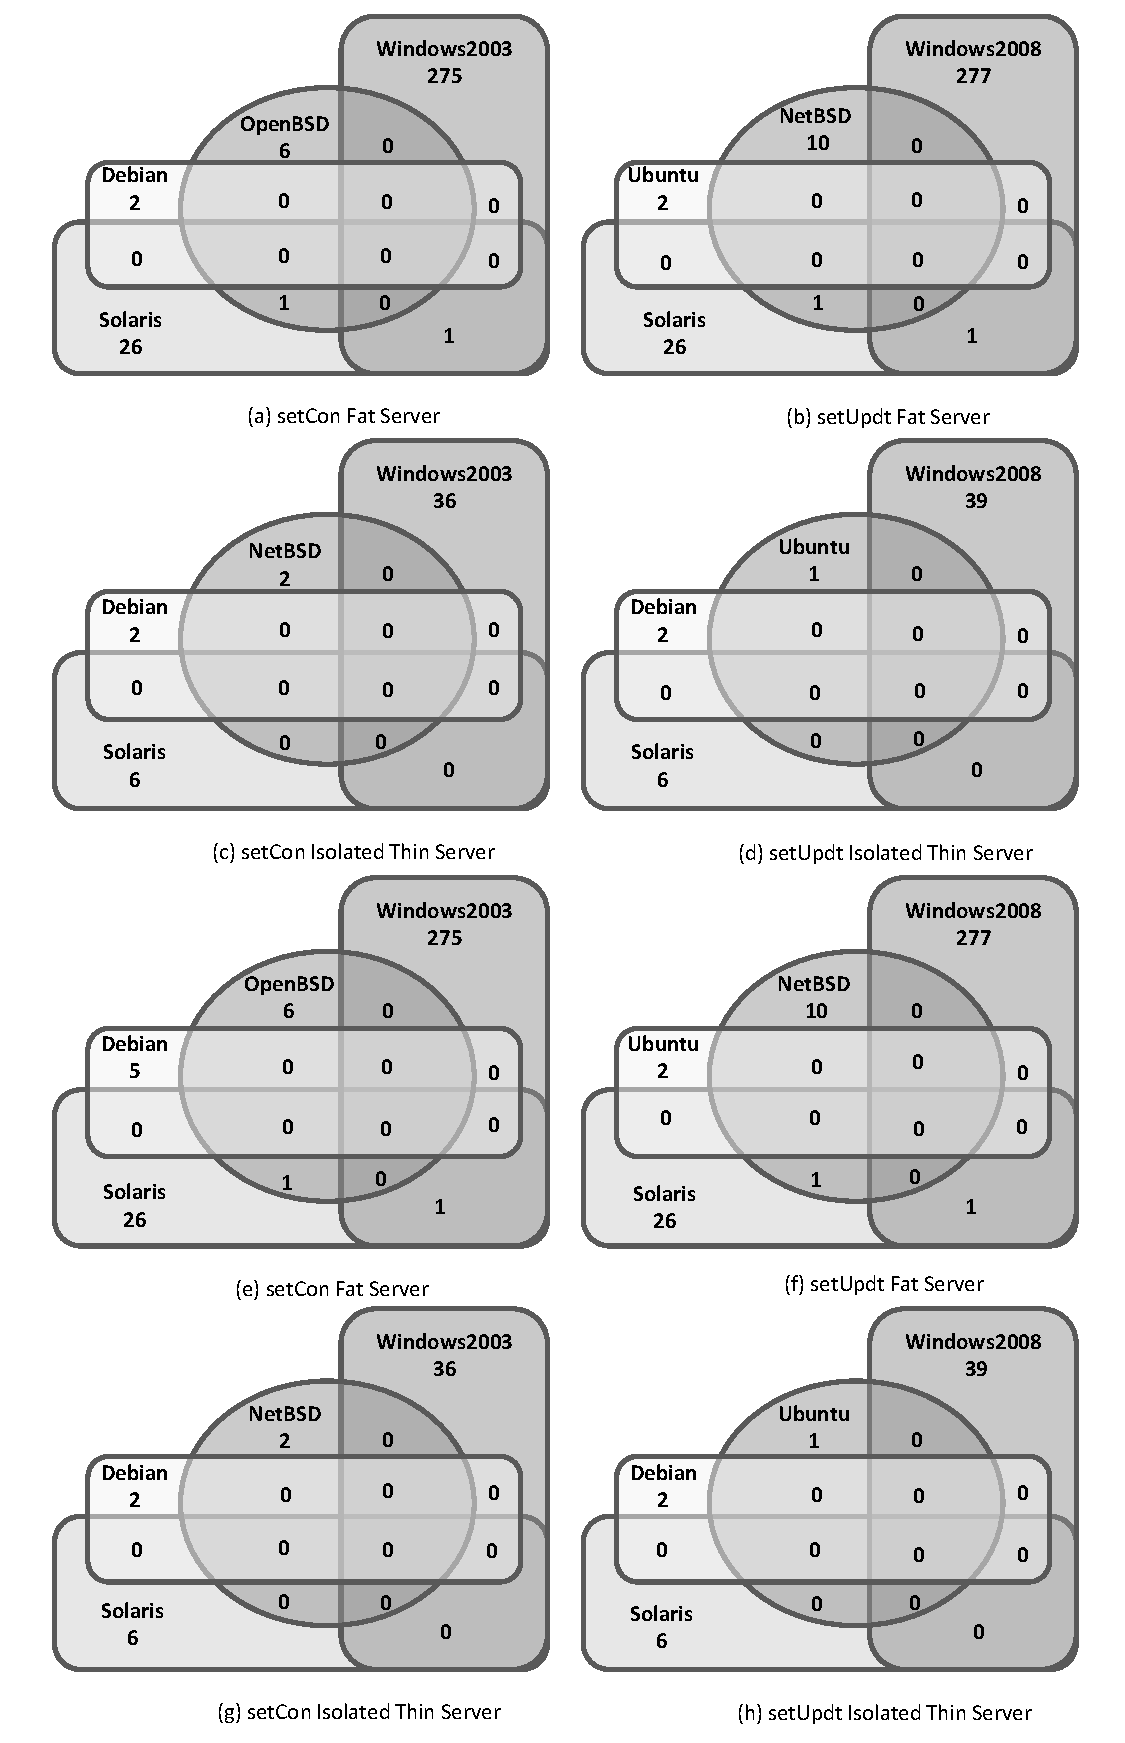
\includegraphics[scale=0.7]{images/images/grayscale_ven_dia_one_fig_update.pdf}
 \caption{Venn diagrams for vulnerabilities in setCon and setUpdt for strategies CVCst and CVIst in Fat Server and Isolated Thin Server configurations. The first four diagrams (a, b, c and d) represent the results for CVC, and the last four \glspl{os} (e, f, g and h) represent the results for CVI.}
 \label{fig-venn}
\end{figure}


\subsubsection*{Common Vulnerability Indicator Strategy (CVIst)} 
This strategy employs the \gls{cvi} value, defined at the beginning of this section, to make decisions about including/excluding particular \glspl{os}.
Therefore, besides taking advantage of the available data on total counts of shared vulnerabilities, it also uses the information on how these numbers have evolved through the years.

\gls{cvis} is applied by executing the following method, which is based on minimizing a cost function. 
For a given year and time span, the \gls{cvi} value is calculated for each of the \gls{os} pairs. 
Typically, one should use the most recent year for which there is available data. 
The time span should cover a reasonable interval so that the indicator reflects the trend of discovered vulnerabilities. 
In some cases, however, one may have to resort to smaller time spans due to lack of data, namely with \glspl{os} released recently. 
In this case, the indicator will give a higher weight to the vulnerabilities reported in the last year. 
In \gls{cvis} the cost of creating a group with two \glspl{os} A and B is $\mathit{CVI}(A,B)$. 
Extending this idea to a group of $n$ \glspl{os}, the total cost becomes the sum of the individual \gls{cvi} for all combinations of \gls{os} pairs.
In order to choose the best groups, the strategy searches for sets of \glspl{os} that together have the smallest total cost.


\begin{table}[!ht]
\begin{center}
{\footnotesize
\begin{tabular}{|l|c|c|c|c|c|c|c|c|c|c|c|c|}\cline{2-11}
 \multicolumn{1}{c|}{} &
\begin{sideways}\vspace{2mm}\parbox{2mm}OpenBSD\end{sideways}&
\begin{sideways}\vspace{2mm}\parbox{2mm}NetBSD\end{sideways}&
\begin{sideways}\vspace{2mm}\parbox{2mm}FreeBSD\end{sideways}&
\begin{sideways}\vspace{2mm}\parbox{2mm}Solaris  \end{sideways}&
\begin{sideways}\vspace{2mm}\parbox{2mm}Debian\end{sideways}&
\begin{sideways}\vspace{2mm}\parbox{2mm}Ubuntu \end{sideways}&
\begin{sideways}\vspace{2mm}\parbox{2mm}Red Hat\end{sideways}&
\begin{sideways}\vspace{2mm}\parbox{3mm}Win2000 \end{sideways}&
\begin{sideways}\vspace{2mm}\parbox{3mm}Win2003 \end{sideways}&
\begin{sideways}\vspace{2mm}\parbox{3mm}Win2008  \end{sideways}&
\multicolumn{2}{|c}{} \\ \cline{1-11}  \cline{1-12}
OpenBSD & - & 17.1 & 22.2 & 4.0 & 1.7 & 2.5 & 5.0 & 1.8 & 1.5 & 0.9 & \multirow{13}{1mm}{\begin{sideways}\hspace{8mm}\parbox{16mm}{$\mathit{CVI}_{2009}$(A,B)}\end{sideways}} \\ \cline{1-11}
NetBSD & 4 &  - & 19.7 & 4.9 & 1.4 & 0.0 & 1.8 & 1.6 & 1.5 & 0.9&\\ \cline{1-11}
FreeBSD & 4 & 6 & - & 6.5 & 1.3 & 1.3 & 5.6 & 2.3 & 2.0 & 0.9&\\ \cline{1-11}
Solaris & 1 & 1 & 2 & - & 1.0 & 1.5 & 5.3 & 5.5 & 5.6 & 0.0&\\ \cline{1-11}
Debian & 0 & 0 & 0 & 0 & - & 10.5 & 26.1 & 0.9 & 0.9 & 0.0&\\ \cline{1-11}
Ubuntu & 0 & 0 & 0 & 0 & 0 & - & 18.5 & 0.9 & 0.9 & 0.0&\\ \cline{1-11}
Red Hat & 0 & 0 & 0 & 2 & 0 & 0 &  - & 1.4 & 1.8 & 0.0&\\ \cline{1-11}
Win2000 & 0 & 0 & 0 & 1 & 0 & 0 & 0 & - & 163.6 & 39.5&\\ \cline{1-11}
Win2003 & 0 & 0 & 0 & 1 & 0 & 0 & 0 & 49 & - & 0.0 &\\ \cline{1-12}
Win2008 & 0 & 0 & 0 & 1 & 0 & 0 & 0 & 38 & 229 & - &\multicolumn{1}{|c}{}  \\ \cline{1-11}
 \multicolumn{1}{c|}{}& \multicolumn{9}{|c|}{2010-2011} & \multicolumn{2}{|c}{}\\ \cline{2-10}
\end{tabular}
\caption{History/observed period for CVIst with Fat Servers.}
\label{tab:strat_ii}
}
\end{center}
\end{table}

To evaluate this strategy, we split the time into two intervals as we did for \gls{cvcs}. 
Table~\ref{tab:strat_ii} presents in the cells for the history period the $\mathit{CVI}_{2009}(A,B)$ for a time span of 10 years in a Fat Server configuration\footnote{In some cases, we had to use smaller time spans due to the more recent release date of the \glspl{os} (e.g., Ubuntu and Windows 2008). When this happened, the CVI value was calculated using the maximum time span that is allowed by the available data.}. 
The cells at left and bottom of the diagonal line correspond to the observed period, and they count as before the number of shared vulnerabilities in 2010 and 2011. After applying \gls{cvis}, the following sets are the best with four \glspl{os}:

\begin{itemize}
\item setCon = \{\emph{OpenBSD, Solaris, Debian, Windows2003}\}, with a total cost of $14.7$;
\item setUpdt = \{\emph{NetBSD, Solaris, Ubuntu, Windows2008}\}, with a total cost of $7.3$.
\end{itemize}

To verify if \gls{cvi} is a good indicator for selecting diverse sets, we can look at the number of common vulnerabilities in the observed period (2010--2011). 
By analyzing Table~\ref{tab:strat_ii}, it is possible to see that setCon and setUpdt remain good sets, each one with two shared flaws. 
As before with CVCst, one can find better sets in observed period, where no vulnerabilities appear in common, for example by replacing Solaris with Red Hat.
The Venn diagrams for these two sets are shown in Figures~\ref{fig-venn}(e) and~\ref{fig-venn}(f).

\begin{table}[!ht]
\begin{center}
{\footnotesize
\begin{tabular}{|l|c|c|c|c|c|c|c|c|c|c|c|c|}\cline{2-11}
 \multicolumn{1}{c|}{} &
\begin{sideways}\vspace{2mm}\parbox{2mm}OpenBSD\end{sideways}&
\begin{sideways}\vspace{2mm}\parbox{2mm}NetBSD\end{sideways}&
\begin{sideways}\vspace{2mm}\parbox{2mm}FreeBSD\end{sideways}&
\begin{sideways}\vspace{2mm}\parbox{2mm}Solaris  \end{sideways}&
\begin{sideways}\vspace{2mm}\parbox{2mm}Debian\end{sideways}&
\begin{sideways}\vspace{2mm}\parbox{2mm}Ubuntu \end{sideways}&
\begin{sideways}\vspace{2mm}\parbox{2mm}Red Hat\end{sideways}&
\begin{sideways}\vspace{2mm}\parbox{3mm}Win2000 \end{sideways}&
\begin{sideways}\vspace{2mm}\parbox{3mm}Win2003 \end{sideways}&
\begin{sideways}\vspace{2mm}\parbox{3mm}Win2008  \end{sideways}&
\multicolumn{2}{|c}{} \\ \cline{1-11}  \cline{1-12}
OpenBSD & - & 8.4 & 14.1 & 1.8 & 0.0 & 0.0 & 1.6 & 1.8 & 1.8 & 0.9  & \multirow{13}{1mm}{\begin{sideways}\hspace{8mm}\parbox{16mm}{$\mathit{CVI}_{2009}$(A,B)}\end{sideways}} \\ \cline{1-11}
NetBSD & 1 & - & 11.0 & 1.5 & 0.6 & 0.0 & 0.6 & 1.6 & 0.9 & 0.9&\\ \cline{1-11}
FreeBSD & 1 & 1 & - & 2.3 & 0.0 & 0.0 & 1.7 & 2.3 & 1.5 & 0.9&\\ \cline{1-11}
Solaris & 0 & 0 & 0 & - & 0.0 & 0.0 & 1.0 & 1.0 & 0.6 & 0.0&\\ \cline{1-11}
Debian & 0 & 0 & 0 & 0 & - & 1.9 & 3.2 & 0.9 & 0.9 & 0.0&\\ \cline{1-11}
Ubuntu & 0 & 0 & 0 & 0 & 0 &  - & 0.9 & 0.9 & 0.9 & 0.0&\\ \cline{1-11}
Red Hat & 0 & 0 & 0 & 0 & 0 & 0 &- & 0.9 & 0.9 & 0.0&\\ \cline{1-11}
Win2000 & 0 & 0 & 0 & 0 & 0 & 0 & 0 & - & 58.7 & 12.5&\\ \cline{1-11}
Win2003 & 0 & 0 & 0 & 0 & 0 & 0 & 0 & 4 & - & 13.5&\\ \cline{1-12}
Win2008 & 0 & 0 & 0 & 0 & 0 & 0 & 0 & 3 & 26 & -&\multicolumn{1}{|c}{}  \\ \cline{1-11}
 \multicolumn{1}{c|}{}& \multicolumn{9}{|c|}{2010-2011} & \multicolumn{2}{|c}{}\\ \cline{2-10}
\end{tabular}
\caption{History/observed period for CVIst with Isolated Thin Servers.}
\label{tab:strat_ii_iso}
}
\end{center}
\end{table}




Table \ref{tab:strat_ii_iso} provides the data for applying CVIst in Isolated Thin Server configurations. 
It is possible to observe that \gls{cvi} values have significantly decreased when compared to the previous table. 
The best groups of four \glspl{os} in the historical period are:
 
\begin{itemize}
\item setCon = \{\emph{NetBSD, Solaris, Debian, Windows2003}\}, with a total cost of $4.5$;
\item setUpdt = \{\emph{Solaris, Debian, Ubuntu, Windows2008}\}, with a total cost of $1.9$.
\end{itemize}

By checking the data for the observed period, one can see that both sets do not share a single vulnerability, which indicates that the strategy would have made a good selection of \glspl{os} (see also the Venn diagrams in Figures~\ref{fig-venn}(g) and~\ref{fig-venn}(h)).

%TABLE VII

\begin{table}[!ht]
\begin{center}
{\scriptsize
\begin{tabular}{|l||c c c c c|}\hline
&	0 $\leq$ IRT $\leq 1$	&	$1$ \textless IRT $\leq 10$	&	$10$ \textless IRT $\leq100$	&	$100$ \textless IRT $\leq 1000$	& $1000$ \textless IRT $\leq10000$\\\hline
OpenBSD-Win2008 & 0 & 0 & 0 & 0 & 0 \\
NetBSD-Ubuntu & 0 & 0 & 0 & 0 & 0 \\
NetBSD-Win2003 & 0 & 0 & 0 & 0 & 0 \\
NetBSD-Win2008 & 0 & 0 & 0 & 0 & 0 \\
FreeBSD-Win2008 & 0 & 0 & 0 & 0 & 0 \\
Solaris-Win2008 & 0 & 0 & 0 & 0 & 0 \\
Debian-Win2000 & 0 & 0 & 0 & 0 & 0 \\
Debian-Win2003 & 0 & 0 & 0 & 0 & 0 \\
Debian-Win2008 & 0 & 0 & 0 & 0 & 0 \\
Ubuntu-Win2000 & 0 & 0 & 0 & 0 & 0 \\
Ubuntu-Win2003 & 0 & 0 & 0 & 0 & 0 \\
Ubuntu-Win2008 & 0 & 0 & 0 & 0 & 0 \\
Red Hat-Win2008 & 0 & 0 & 0 & 0 & 0 \\ \hline
OpenBSD-Win2003 & 0 & 0 & 0 & 0 & 1 \\
FreeBSD-Win2003 & 0 & 0 & 0 & 0 & 1 \\
Solaris-Debian & 0 & 0 & 0 & 0 & 1 \\
Red Hat-Win2000 & 0 & 0 & 0 & 0 & 1 \\
OpenBSD-Win2000 & 0 & 0 & 0 & 0 & 2 \\ \hline
OpenBSD-Debian & 0 & 0 & 0 & 1 & 0 \\
Solaris-Ubuntu & 0 & 0 & 0 & 1 & 0 \\
NetBSD-Win2000 & 0 & 0 & 0 & 1 & 1 \\
FreeBSD-Win2000 & 0 & 0 & 0 & 2 & 1 \\ \hline
FreeBSD-Ubuntu & 0 & 0 & 1 & 0 & 0 \\
Red Hat-Win2003 & 0 & 0 & 1 & 0 & 0 \\
OpenBSD-Solaris & 0 & 0 & 3 & 4 & 2 \\
FreeBSD-Solaris & 0 & 0 & 5 & 8 & 0 \\ \hline
FreeBSD-Debian & 0 & 1 & 0 & 2 & 0 \\ \hline
OpenBSD-Ubuntu & 1 & 0 & 0 & 1 & 0  \\
NetBSD-Debian & 1 & 0 & 0 & 1 & 0 \\
NetBSD-Solaris & 1 & 0 & 3 & 4 & 1 \\
Solaris-Win2003 & 1 & 1 & 1 & 4 & 0 \\
Solaris-Win2000 & 1 & 1 & 1 & 4 & 1 \\
NetBSD-Red Hat & 2 & 0 & 0 & 3 & 0 \\
Solaris-Red Hat & 2 & 0 & 0 & 7 & 0\\
FreeBSD-Red Hat & 2 & 1 & 2 & 5 & 1\\
Debian-Ubuntu & 3 & 2 & 3 & 5 & 0\\
OpenBSD-Red Hat & 4 & 0 & 1 & 4 & 0\\
NetBSD-FreeBSD & 4 & 3 & 20 & 14 & 0 \\
OpenBSD-NetBSD & 7 & 3 & 14 & 12 & 0 \\
Ubuntu-Red Hat & 11 & 2 & 7 & 6 & 0 \\
OpenBSD-FreeBSD & 11 & 5 & 16 & 14 & 0 \\
Debian-Red Hat & 22 & 3 & 18 & 8 & 0 \\
Win2000-Win2008 & 54 & 7 & 15 & 3 & 0 \\
Win2000-Win2003 & 167 & 29 & 66 & 2 & 0 \\
Win2003-Win2008 & 222 & 16 & 41 & 2 & 0 \\ \hline
\end{tabular}
\caption{Number of two consecutive vulnerabilities occurring in each \gls{irt} period, between 2000 and 2011 (with Fat Servers).}
\label{tab:pairs_irt}
}
\end{center}
\end{table}



\subsubsection*{Inter-Reporting Times Strategy (IRTst)} \label{IRT} 
This strategy is mainly concerned with the \emph{\gls{irt}}, i.e., the number of days between successive reports of common vulnerabilities in different \gls{os} pairs, rather than vulnerability counts. 
The assumption underlying this strategy is that lower inter-reporting times suggest a greater similarity between \glspl{os}, and thus it would be advisable, from a diversity standpoint, to select \glspl{os} with higher \gls{irt}.

Table \ref{tab:pairs_irt} presents the number of vulnerabilities for each pair of \glspl{os} in five \gls{irt} intervals, from 0 to 10000 days.
The values in the table were obtained in the following manner: first, for a given \gls{os} pair A and B, we collected the dates for common vulnerabilities; next, we calculated the \gls{irt} in days of every two consecutive vulnerabilities; and then, we counted the number of vulnerabilities that were within each interval.
The table is organized such that on the top are the \glspl{os} without common vulnerabilities, which are then followed by the ones that had larger \gls{irt} values. 
Therefore, each horizontal line separates groups of \gls{os} pairs that have positive \gls{irt} values in the same leftmost column, starting from the rightmost column (i.e., with the longer \gls{irt}). 
From a diversity perspective, it is interesting to notice that in the table there are $29\%$ of the pairs that do not have two consecutive vulnerabilities, and that $11\%$ only have consecutive vulnerabilities from $1000$ days on (last column).

The \gls{irts} strategy allows the selection of \glspl{os} with longer \gls{irt}. 
This criteria is essential if one wants to deploy a system that has a short lifetime, e.g., a batching process, which ideally would only be in operation between the discovery of common vulnerabilities. 
\gls{irts} tries first to select \gls{os} pair with zero common vulnerabilities; when this is not possible, it chooses next pair whose common vulnerabilities appear in the rightmost columns. 
By inspecting the table, we can see that the best two sets of four \glspl{os} are:

\begin{itemize}
\item setCon = \{\emph{OpenBSD, Solaris, Debian, Windows2003}\};
\item setUpdt = \{\emph{NetBSD, Solaris, Ubuntu, Windows2008}\}.
\end{itemize}


Table \ref{tab:pairs_irt_iso} presents the \gls{irt} for an Isolated Thin Server configuration. 
Since each \gls{os} pair has less common vulnerabilities, this often translates to larger \gls{irt}.  
The percentage of lines with zero \gls{irt} in all intervals is higher, $51\%$, but remained the same for the \gls{os} pairs that share vulnerabilities with longer \gls{irt} ($11\%$). 
When applying the strategy to this table, the best sets of \glspl{os} are: 

\begin{itemize}
\item setCon = \{\emph{OpenBSD, Solaris, Debian, Windows2003}\};
\item setUpdt = \{\emph{OpenBSD, Debian, Ubuntu, Windows2008}\}.
\end{itemize}


\begin{table}[!ht]
\begin{center}
{\scriptsize
\begin{tabular}{|l||c c c c c|}\hline
&	$0$ $\leq$ IRT $\leq 1$	& $1$ \textless IRT $\leq 10$ & $10$ \textless IRT $\leq 100$ & $100$ \textless IRT $\leq 1000$ & $1000$ \textless IRT $\leq 10000$\\\hline
OpenBSD-Debian & 0 & 0 & 0 & 0 & 0 \\
OpenBSD-Ubuntu & 0 & 0 & 0 & 0 & 0 \\
OpenBSD-Win2008 & 0 & 0 & 0 & 0 & 0 \\
NetBSD-Ubuntu & 0 & 0 & 0 & 0 & 0 \\
NetBSD-Win2003 & 0 & 0 & 0 & 0 & 0 \\
NetBSD-Win2008 & 0 & 0 & 0 & 0 & 0 \\
FreeBSD-Debian & 0 & 0 & 0 & 0 & 0 \\
FreeBSD-Ubuntu & 0 & 0 & 0 & 0 & 0 \\
FreeBSD-Win2008 & 0 & 0 & 0 & 0 & 0 \\
Solaris-Debian & 0 & 0 & 0 & 0 & 0 \\
Solaris-Ubuntu & 0 & 0 & 0 & 0 & 0 \\
Solaris-Win2003 & 0 & 0 & 0 & 0 & 0 \\
Solaris-Win2008 & 0 & 0 & 0 & 0 & 0 \\
Debian-Win2000 & 0 & 0 & 0 & 0 & 0 \\
Debian-Win2003 & 0 & 0 & 0 & 0 & 0 \\
Debian-Win2008 & 0 & 0 & 0 & 0 & 0 \\
Ubuntu-Red Hat & 0 & 0 & 0 & 0 & 0 \\
Ubuntu-Win2000 & 0 & 0 & 0 & 0 & 0 \\
Ubuntu-Win2003 & 0 & 0 & 0 & 0 & 0 \\
Ubuntu-Win2008 & 0 & 0 & 0 & 0 & 0 \\
Red Hat-Win2000 & 0 & 0 & 0 & 0 & 0 \\
Red Hat-Win2003 & 0 & 0 & 0 & 0 & 0  \\
Red Hat-Win2008 & 0 & 0 & 0 & 0 & 0 \\ \hline
OpenBSD-Win2003 & 0 & 0 & 0 & 0 & 1 \\
FreeBSD-Win2003 & 0 & 0 & 0 & 0 & 1 \\
Solaris-Red Hat & 0 & 0 & 0 & 0 & 1 \\
Solaris-Win2000 & 0 & 0 & 0 & 0 & 1  \\
OpenBSD-Win2000 & 0 & 0 & 0 & 0 & 2 \\ \hline
Debian-Ubuntu & 0 & 0 & 0 & 1 & 0 \\
NetBSD-Win2000 & 0 & 0 & 0 & 1 & 1 \\
FreeBSD-Win2000 & 0 & 0 & 0 & 2 & 1 \\ \hline
NetBSD-Solaris & 0 & 0 & 1 & 2 & 0 \\
OpenBSD-Solaris & 0 & 0 & 1 & 3 & 0 \\
FreeBSD-Solaris & 0 & 0 & 1 & 4 & 0 \\ \hline
NetBSD-Debian & 1 & 0 & 0 & 0 & 0  \\
NetBSD-Red Hat & 1 & 0 & 0 & 0 & 0 \\
Debian-Red Hat & 1 & 0 & 1 & 3 & 2 \\
OpenBSD-Red Hat & 2 & 0 & 0 & 0 & 0 \\
FreeBSD-Red Hat & 2 & 0 & 0 & 0 & 0 \\
OpenBSD-NetBSD & 2 & 0 & 3 & 7 & 1 \\
NetBSD-FreeBSD & 2 & 0 & 6 & 9 & 1 \\
OpenBSD-FreeBSD & 6 & 0 & 9 & 10 &  1\\
Win2000-Win2008 & 8 & 1 & 3 & 3 & 0 \\
Win2003-Win2008 & 16 & 2 & 19 & 2 & 0 \\
Win2000-Win2003 & 35 & 8 & 36 & 5 & 0\\ \hline
\end{tabular}
\caption{Number of two consecutive vulnerabilities occurring in each IRT period, between 2000 and 2011 (Isolated Thin Servers).}
\label{tab:pairs_irt_iso}
}
\end{center}
\end{table}

\subsubsection*{Comparing the three strategies}
The three strategies explore distinct characteristics of the data to pick the \glspl{os} to be deployed. 
Qualitatively they differ in the method of selection, and potentially the result of applying them to our data could lead to distinct sets being chosen.
On the other hand, they all try to find \glspl{os} that when placed together in the same system have a low probability of experiencing common vulnerabilities in the future. 
Therefore, if there is a small collection of \gls{os} sets with this property, then all strategies should elect one of these sets as the best choice. 
This is precisely what we observed with the \gls{nvd} data, and consequently, the selected best sets are not too different from each other.
Only when one needs to find many \gls{os} sets with reasonable levels of diversity, such as with the implementation of proactive recovery mechanisms in intrusion-tolerant systems \cite{Castro:2002,Sousa:2010}, then the distinctions among the strategies start to become apparent.
We leave it as future work a more refined study on the comparison of the strategies with larger groups of \gls{os} sets.

The \gls{os} sets that resulted from the execution of the strategies achieved reasonable levels of diversity when evaluated in the observed period (years 2010 and 2011). 
As expected from our analysis, several of the best sets contained an \gls{os} from each of the families. 
The exception to this rule occurred with the Linux family, wherein a few cases it had two representatives (Debian and Ubuntu) because these \glspl{os} had very few vulnerabilities reported in the last three years. 
Even though the BSD family also had a small number of recent vulnerabilities, since these occasionally affected more \glspl{os}, the strategies opted for including just one of the BSD \glspl{os}.

In the next section, we will look into \gls{os} versions as a way to increase diversity. 
For this study, we will use the set that was most selected by the different strategies: \{\emph{OpenBSD, Debian, Solaris, Windows2003}\} (4 out of 12 choices, considering both Fat Server and Isolated Thin Server configurations).


%%%%%%%%%%%%%%%%%%%%%%%%%%%%%%%%%%%%%%%%%%%%%%%%%%%%%%%%%%%%%%%%%%%%%%%%%%%%%%%%%%%%%%%%%%%
\subsection{Exploring Diversity Across OS Releases}
\label{releases}

If one wants to build systems capable of tolerating a few intrusions, our results show that it is possible to select \glspl{os} for the replicas with a small collection of common vulnerabilities. 
It is hard, however, to support critical services that need to remain correct with higher numbers of compromised replicas or to use some \gls{bft} algorithms that trade off performance for extra replicas (e.g., \cite{Abd-El-Malek:2005,Kotla:2010,Serafini:2010}). 
The number of available \glspl{os} is limited, and consequently, one rapidly runs out of different \glspl{os} (e.g., 13 distinct \glspl{os} are needed to tolerate $f=4$ faults in a $3f+1$ system). 
On the other hand, our experiments are relatively pessimistic in the sense that they are based on long periods of time, and no distinctions are made between \gls{os} releases.

Newer releases of an \gls{os} can contain essential code changes, and therefore, old vulnerabilities may disappear and/or new vulnerabilities may be introduced. 
As a result, if we consider (OS, release) pairs, one may augment the number of different systems that do not share vulnerabilities. 
Nevertheless, one should keep in mind that the use of older \gls{os} releases does not come without a cost. Namely, there might be incompatibilities with the current hardware, and some older software packages might be challenging to find.

In the next two sections we explore \emph{n-diverse} sets, where we extend the OS, as an element in the set, to the \gls{os} release. 
First we study a \emph{4-diverse} set, and then a \emph{2-diverse} set built with only two \glspl{os}. 
We will concentrate on Isolated Thin Server configurations because they correspond to the most common way to deploy intrusion-tolerant systems.


\subsubsection*{4-diverse sets}
Here we analyze in more detail the vulnerabilities for the set \{\emph{OpenBSD, Debian, Solaris, Windows2003}\} across their releases between 2000 and 2011. 
Despite the year of the release, since some vulnerabilities can be inherited from older versions of the code, we will include all vulnerabilities no matter the published date (i.e., even the flaws before 2000).

From all releases available for our 4-version replicated system,\footnote[1]{OpenBSD~2.7, OpenBSD~2.8, OpenBSD~2.9, OpenBSD~3.0, OpenBSD~3.1, OpenBSD~3.2, OpenBSD~3.3, OpenBSD~3.4, OpenBSD~3.5, OpenBSD~3.6, OpenBSD~3.7, OpenBSD~3.8 OpenBSD~3.9, OpenBSD~4.0, OpenBSD~4.1, OpenBSD~4.2, OpenBSD~4.3, OpenBSD~4.4,   Solaris~10.0, Solaris~11.0, Solaris~8.0, Solaris~8.1, Solaris~8.2, Solaris~9.0, Solaris~9.1, Debian~2.2, Debian~2.3, Debian~3.0,   Debian~3.1, Debian~4.0, Debian~6.0, Debian~6.2, and Windows~2003.} we looked at the major releases that had non-zero vulnerabilities. 
Since OpenBSD follows a fixed six-month release cycle, in this case, we selected one version every three years, which is reasonable given our 12-year time span (considering all 18 releases would require 154 entries in the table). 
Therefore, the \gls{os} releases that are taken into the study are: OpenBSD 5.0, OpenBSD 4.4, OpenBSD 3.8, OpenBSD 3.2, Solaris 8.0, Solaris 9.0, Solaris 10.0, Solaris 11.0, Debian 2.2, Debian 3.0, Debian 4.0, Debian 5.0, Debian 6.0 and Windows2003.

\begin{table}[!ht]
\begin{center}
{\scriptsize
\begin{tabular}{|l|c|}\hline
\textbf{OS Versions} & Total  \\\hline\hline
Solaris 8.0-Solaris 9.0 	&21\\
Solaris 9.0-Solaris 10.0 	&8\\
Solaris 8.0-Solaris 10.0 	&7\\
OpenBSD 3.2-OpenBSD 3.8 & 4 \\
OpenBSD 3.2-Solaris 9.0 & 2 \\
OpenBSD 3.2-Windows2003 & 2 \\
OpenBSD 3.2-Solaris 8.0 & 1 \\
OpenBSD 3.8-Windows2003 & 1 \\
Solaris 8.0-Windows2003 & 1 \\
Solaris 9.0-Windows2003 & 1 \\
Solaris 10.0-Windows2003 & 1 \\
Solaris 10.0-Solaris 11.0	& 1 \\
Solaris 8.0-Debian 2.2 &	1 \\
Debian 4.0-Windows2003 & 1 \\\hline
\end{tabular}
\caption{Common vulnerabilities between OS releases.}
\label{tab:vulns_releases}
}
\end{center}
\end{table}

Table \ref{tab:vulns_releases} shows the number of common vulnerabilities for each pair of OS-release (pairs with zero values are not displayed). 
The first observation is that there are many releases within this set of 4 \glspl{os} that appear to be free of common flaws. 
Second, these shared bugs occur more often between releases of the same \gls{os}. 
This is anticipated because more code is re-used within the same \gls{os}.
Additionally, one can notice that releases of the same \gls{os} typically have less shared vulnerabilities when comparing older and newer versions. 
This is particularly evident for the OpenBSD and Debian releases. 
This result is quite promising because it supports our thesis that one should be able to explore diversity across releases, as a way to increase the number of available candidates for the construction of the diverse \gls{os} sets.


\subsubsection*{2-diverse sets} 
To reduce the development and maintenance costs of an intrusion-tolerant system, it is reasonable to investigate solutions that attempt to decrease the number of distinct \glspl{os} but still ensure a high level of security. 
Here, it makes sense to consider an approach that offers diversity with only two \glspl{os}, while still exploiting the diversity available within the \gls{os} releases. 
In the extreme case, one can select \glspl{os} from the same family, for instance, to simplify system management.

To study this sort of solution, we looked at the vulnerabilities that appeared in several versions of Debian and Red Hat (all released after 2000). 
In total, seven Debian and ten Red Hat releases were considered, which gives a total of $136$ combinations. 
Table \ref{tab:debian_RedHat} provides a summary of the vulnerabilities that were found in \gls{nvd} for pairs of \gls{os} releases (to save space, we omit pairs with zero common vulnerabilities). 
The reader should notice that Red Hat went through two distinct distributions from 2000, and they can be distinguished by the version number: Red Hat Linux existed between 2000 and 2003, and it has a dot in the version number (e.g., Red Hat 7.1); Red Hat Enterprise Linux is available from 2003, and its releases only have a single digit (e.g., Red Hat 3).

\begin{table}[!ht]
\begin{center}
{\scriptsize
\begin{tabular}{|l|c||l|c|}\hline
\textbf{OS Versions} & Total &  \textbf{OS Versions} & Total \\\hline\hline
Debian 2.2 - Debian 2.3 & 2 & Red Hat 7.1 - Red Hat 9.0 & 2  \\\hline
Debian 3.1 - Debian 4.0 & 1 & Red Hat 7.2 - Red Hat 7.3 & 5  \\\hline
Debian 4.0 - Red Hat 3 & 1 &  Red Hat 7.2 - Red Hat 8.0 & 5  \\\hline
Debian 4.0 - Red Hat 4 & 1 & Red Hat 7.2 - Red Hat 9.0 & 2  \\\hline
Debian 4.0 - Red Hat 5 & 1 & Red Hat 7.3 - Red Hat 8.0 & 5  \\\hline
Red Hat 7.0 - Red Hat 7.1 & 2 & Red Hat 7.3 - Red Hat 9.0 & 2  \\\hline
Red Hat 7.0 - Red Hat 7.2 & 1 & Red Hat 8.0 - Red Hat 9.0 & 2  \\\hline
Red Hat 7.1 - Red Hat 7.2 & 3 &  Red Hat 3 - Red Hat 4 & 2  \\\hline
Red Hat 7.1 - Red Hat 7.3 & 2 & Red Hat 3 - Red Hat 5 & 1  \\\hline
Red Hat 7.1 - Red Hat 8.0 & 2 &  Red Hat 4 - Red Hat 5 & 1  \\\hline
\end{tabular}
\caption{Common vulnerabilities between Debian and Red Hat releases.}
\label{tab:debian_RedHat}
}
\end{center}
\end{table}

The table only shows $14.7\%$ of the \gls{os} releases combinations, which means $85.3\%$ of the \gls{os} pairs are free from common flaws. 
Debian has very few vulnerabilities that are shared between versions. 
Moreover, accordingly to \gls{nvd}, these few vulnerabilities only affect two releases, i.e., no vulnerability had an impact over an extensive period. 
There are two vulnerabilities, CVE-2003-0248 and CVE-2003-0364, that appear in five Red Hat releases (from Red Hat 7.1 to Red Hat 9.0). 
The first is a vulnerability in the \emph{mxcsr} kernel code which lets attackers modify CPU state registers via a malformed address. 
This is a critical vulnerability because it has an impact on availability, confidentiality, and integrity. 
The second one is in the Red Hat TCP/IP implementation, and allows a \gls{dos} by CPU consumption. 
Three vulnerabilities occur in Red Hat 7.2, 7.3 and 8.0, all related to particular versions and configurations of the OpenSSL cryptographic toolkit. 
When exploited, they cause a \gls{dos} (CVE-2004-0079, CVE-2004-0081 and CVE-2004-0112).
%Again, we can observe that few high impact vulnerabilities cross many versions of the same \gls{os}. 

These results demonstrate that with a careful selection of the Debian and Red Hat releases, it is possible to avoid most of the common vulnerabilities, and apparently, it becomes viable to build an intrusion-tolerant replicated system based on only two \glspl{os}.


\section{Decisions About Deploying Diversity}\label{decisions}
We have underscored that these results are only \textit{prima facie} evidence for the usefulness of diversity. 
On average, we would expect our estimates to be conservative as we analyzed aggregated vulnerabilities across releases: common vulnerabilities could be much smaller in a ``specific set'' of diverse \gls{os} releases. 
However, there are limitations on what can be claimed from the analysis of the \gls{nvd} data alone without further manual analysis (other than what we have done, e.g., developing/finding and running exploit scripts on every \gls{os} for each vulnerability).
A better analysis would be obtained if the \gls{nvd} vulnerability reports were combined with the exploit reports (including exploiting counts), and even better if they also had indications about the users' usage profile.
Moreover, we have seen that \gls{nvd} has some limitations, as we have found that some of the vulnerabilites were not reported in the \gls{nvd}, but several security advisory websites have reported those vulnerabilities.
%However, vendors are often wary of sharing such detailed dependability and security information with their customers.
Additionaly, there are partial exploit reports available from other sites (e.g., \cite{cvedetails}).


Given these limitations, \emph{how can individual user organizations decide whether diversity is a suitable option for them, with their specific requirements and usage profiles?}
The cost is reasonably easy to assess: costs of the software products, the required middleware (if any), added the complexity of management, difficulties with client applications that require vendor-specific features, hardware costs, run-time cost of the synchronization and consistency enforcing mechanisms, and possibly more complex recovery after some failures.
The gains in improved security (from some tolerance to zero-day vulnerabilities and easier recovery from some exploits, set against possible extra vulnerabilities due to the increased complexity of the system) are difficult to predict except empirically. 


The first step onto adopting diversity as a dependable mechanism is done. 
The other limitations will be addressed in the rest of this thesis. 


\section{Final Remmarks}

In this chapter we presented results from an analysis of 18 years (1994--2011) of vulnerability reports from the \gls{nvd}  database. 
We analyzed 2270 vulnerabilities of eleven \gls{os} distributions. 
We enriched the dataset with manual fixes and further classification of vulnerabilities, depending on which part of the \gls{os} they affected, into the kernel, driver, system software, and applications. The enriched dataset allowed us to perform various analysis to answer the main questions that drove our research for this thesis: 
\emph{what are the potential security gains that could be attained from using diverse \glspl{os} in a replicated intrusion-tolerant system?}
 

\chapter{BFT Diversity Management}
\label{chap:lazarus_design}

 \note{We need to clarify that \system is proactive and \sieveq is reactive, they can be used together. E.g., when there is a problem the controller increases the risk}
\section{Introduction}


%This model only works if nodes fail independently, otherwise, once an attacker discovers a vulnerability in one node, it is most likely that the remaining nodes suffer from the same weakness. 

This paper presents \system, the first system that automatically changes the attack surface of a \gls{bft} system in a dependable way.
\system continuously collects security data from \gls{osint} feeds on the internet to build a knowledge base about the possible vulnerabilities, exploits, and patches related to the systems of interest.
This data is used to create clusters of similar vulnerabilities, which potentially can be affected by (variations of) the same exploit.
These clusters and other collected attributes are used to analyze the risk of the \gls{bft} system becoming compromised. % due to common vulnerabilities.
Once the risk increases, \system replaces the potentially vulnerable replica by another one, trying to maximize the failure independence. % of the replicated service.
Then, the replaced node is put on quarantine and updated with the available patches, to be re-used later.
These mechanisms were implemented to be fully automated, removing the human from the loop.

The current implementation of \system manages 17 \gls{os} versions, supporting the \gls{bft} replication of a set of representative applications.
The replicas run in \glspl{vm}, allowing provisioning mechanisms to configure them. 
We conducted two sets of experiments, one demonstrates that \system risk management can prevent a group of replicas from sharing vulnerabilities over time; the other, reveals the potential negative impact that virtualization and diversity can have on performance. However, we also show that if naive configurations are avoided, \gls{bft} applications in diverse configurations can actually perform close to our homogeneous bare metal setup.
%These results open avenues for many future works in the area. 

In summary, we make the following contributions: 

\begin{enumerate}

\item \system, a control plane that monitors \gls{osint} data and manages the \gls{bft} service replicas, selecting and reconfiguring the system to always run the ``most diverse'' set of replicas at any given time (Sections~\ref{sec:design} and~\ref{sec:implementation});

\item A method for assessing the risk of a group of replicas being compromised based on the security news feeds available on the internet. 
The method overcomes limitations from works that use NVD data for managing the replicas vulnerability independence (Section~\ref{sec:metric});

\item An evaluation of our risk management method based on real historical vulnerability data showing its effectiveness in keeping a group of replicas safe from common vulnerabilities (Section~\ref{sec:diversity});

\item An extensive evaluation of \system prototype using 17 \gls{os} versions, a \gls{bft} replication library, and some \gls{bft} applications (i.e., a \gls{kvs}, an application-level firewall/message queuing service, and a blockchain service) showing the costs of supporting diversity in \gls{bft} systems (Section~\ref{sec:overhead}).

\end{enumerate}



In a nutshell, as displayed in~Figure~\ref{fig:overview}, \system provides a distributed operating system for \gls{bft}-replicated services.
The system manages in its execution plane a set of nodes that can run \emph{unmodified replicas} (encapsulated in \glspl{vm} or containers). 
Each node must have a small \gls{ltu} that allows the activation and deactivation of replicas as demanded by the \system \emph{Controller}, in the control plane.
The controller decides which software should run at any given time by monitoring the existing vulnerabilities in the pool of replicas, aiming to minimize the risk of having several nodes being compromised by the same attack.

\begin{figure}[h]
\begin{center}
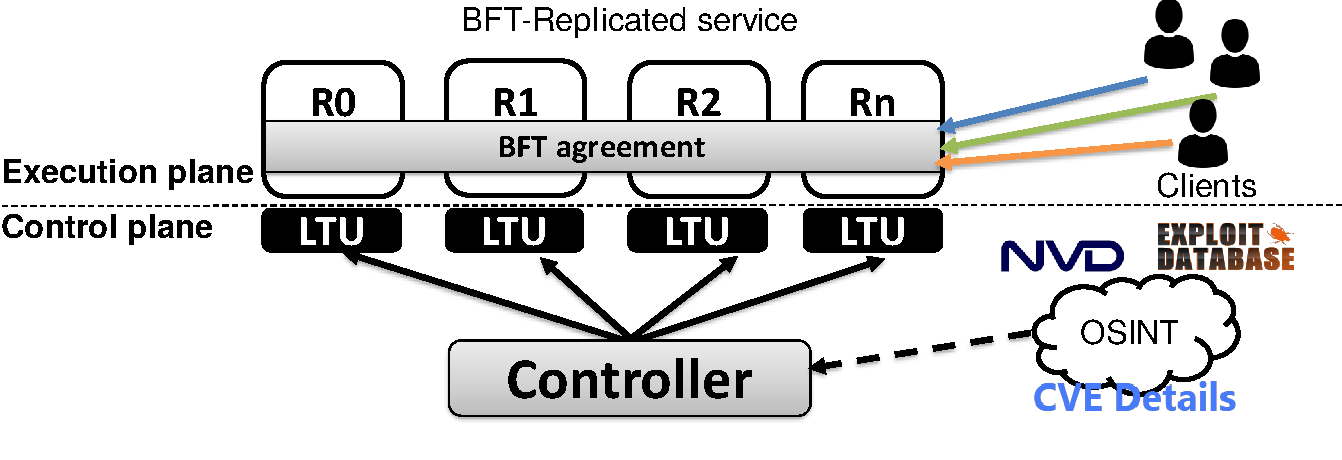
\includegraphics[width=0.7\columnwidth]{images/images/overview.pdf}
\vspace{-5mm}
\caption{\system overview.}
\label{fig:overview}
\end{center}
\end{figure}


\section{System Model}
\label{sec:systemmodel}

\system system model shares some similarity with previous works on the proactive recovery of \gls{bft} systems (e.g.,~\cite{Castro:2002,Platania:2014,Sousa:2010,Roeder:2010}).
More specifically, we consider a \emph{hybrid system model} composed of two planes with different properties and assumptions:

\begin{itemize}

\item \textbf{Execution Plane:} 
This plane is componsed of replica processes that can be subject to Byzantine failures.
Therefore, a Byzantine replica can try to mislead the other replicas or the clients.
These replicas communicate through an asynchronous network that can delay, drop or modify messages, just like most \gls{bft} system models~\cite{Castro:1999,Kotla:2010,Bessani:2014,Aublin:2015}.
This plane hosts $n$ replicas from which at most $f$ can be compromised at any given moment.
In this paper, we consider the typical scenario in which $n=3f+1$~\cite{Castro:2002,Kotla:2010,Aublin:2015}.  

\item \textbf{Control Plane:}  
For simplicity, we will address this component as a logical-centralized controller, which requires stronger assumptions. 
However, in Chapter~\ref{} we introduce \controller which requires weaker assumptions like the Execution Plane.

In this plane, we assume that each component can only fail by crashing. 
Each \emph{node} hosting processes contains a \gls{ltu}, and there is a logically-centralized controller to reconfigure the system, just like what has been used in several previous works on proactive recovery (e.g.,~\cite{Roeder:2010,Platania:2014,Sousa:2010}).
The failures of such components do not compromise the liveness and safety of the service as long as the control plane is recovered before $f$ replicas fail.


\end{itemize}

Besides the execution and control planes, we assume the existence of two types of external components: (1) clients of the replicated service, which can be subject to Byzantine failures; (2) \gls{osint} sources (e.g., \gls{nvd}, ExploitDB) that can not be subverted and controlled by the adversary.
In practice, this assumption lead us consider only well-established and authenticated data sources.
Dealing with untrusted sources is an active area of research in the threat intelligence community (e.g.,~\cite{Sabottke:2015,Liu:2015}), which we consider out of scope for this paper.


\section{Execution Plane}
\label{sec:executionplane}

The Execution Plane can accomodate any replicated system that already levareges on the existence of a controller node (e.g.,~\cite{Sousa:2010,Roeder:2010,Platania:2014,Garcia:2016}) or any \gls{bft} system that would benefit from the \system assistence (e.g.,~\cite{Sousa:2018}). 


\section{Control Plane}
\label{sec:controlplane}

\system is the first control plane that automatically changes the attack surface of a \gls{bft} system in a dependable way.
\system continuously collects security data from \gls{osint} feeds on the internet to build a knowledge base about the possible vulnerabilities, exploits, and patches related to the systems of interest.
This data is used to create clusters of similar vulnerabilities, which potentially can be affected by (variations of) the same exploit.
These clusters and other collected attributes are used to analyze the risk of the \gls{bft} system becoming compromised. % due to common vulnerabilities.
Once the risk increases, \system replaces the potentially vulnerable replica by another one, trying to maximize the failure independence. % of the replicated service.
Then, the replaced node is put on quarantine and updated with the available patches, to be re-used later.
These mechanisms were implemented to be fully automated, removing the human from the loop.

The current implementation of \system manages 17 \gls{os} versions, supporting the \gls{bft} replication of a set of representative applications.
The replicas run in \glspl{vm}, allowing provisioning mechanisms to configure them. 
We conducted two sets of experiments, one demonstrates that \system risk management can prevent a group of replicas from sharing vulnerabilities over time; the other, reveals the potential negative impact that virtualization and diversity can have on performance. 
However, we also show that if naive configurations are avoided, \gls{bft} applications in diverse configurations can actually perform close to our homogeneous bare metal setup.

\section{Diversity of Replicas}
\label{sec:diversityofreplicas}

%BFT-replicated services running on \system are composed by $n$ replicas.
For our purposes, each \replica is composed of a stack of software, including an OS (kernel plus other software contained in an \gls{os} distribution), execution support (e.g., \gls{jvm}, \gls{dbms}), a \gls{bft} library, and the service that is provided by the system.
%(see Figure~\ref{fig:arch1}).
The set of $n$ replicas is called a \configuration.

It is possible to improve the \replicas fault independence by resorting to different \gls{ots} components in the software stack~\cite{Deswarte:1998}. 
For example, it has been shown that using distinct \glspl{os}~\cite{Garcia:2014}, filesystems~\cite{Rodrigues:2001,Bairavasundaram:2009,Alagappan:2016}, and databases~\cite{Gashi:2007}, can yield important benefits in terms of fault independence. In addition, automatic techniques could enhance diversity, like randomization/obfuscation of \glspl{os}~\cite{Roeder:2010} and applications~\cite{King:2016}.

Although \system can exploit automatic techniques, in this paper we center our attention on diverse \gls{ots} components. 
In particular, \system monitors the disclosed vulnerabilities of all elements of the software stacks of the replicas to assess which of them may contain common vulnerabilities.  

However, in the experimental evaluation, we focus on the diversity of OSes (not only the kernel, but the whole product) for three fundamental reasons: (1) by far, most of the replica’s code is the \gls{os}; (2) such size and importance, make \glspl{os} a valuable target, with new vulnerabilities and exploits being discovered every day; and (3) there are many options of OSes that can be used.
The two last factors are particularly important to enrich the validity of our analysis.

Moreover, we do not explicitly consider the diversity of the \gls{bft} library (i.e., the protocol implementation) or the service code implemented on top of it.
Four facts justify this decision: (1) N-version programming is too costly for this~\cite{Avizienis:1977}; (2) there have been some works showing that such protocol implementations can be generated from formally verified specifications~\cite{Hawblitzel:2015,Rahli:2018}; (3) the relatively small size of such components (e.g., a key-value store on top of BFT-SMaRt has less than 15k lines of code~\cite{Bessani:2014}) make them relatively simple to test and assess with some confidence~\cite{Martins:2013,Lee:2014};  and (4) there are no reported vulnerabilities about these system to support our study.
Notice that, although we do not explicitly consider the diversity of \gls{bft} libraries, nothing prevents \system from monitoring them (when several alternatives become available). 
Additionally, as a pragmatic approach, we could employ automatic diversity techniques in this layer~\cite{Platania:2014,Roeder:2010}.




\section{Diversity-aware Reconfigurations}
\label{sec:metric}

The core of \system is the vulnerability evaluation method used to assess the risk of having replicas with shared vulnerabilities.
This section details this method.

\subsection{Finding Common Vulnerabilities}

%\gls{nist}'s \gls{nvd}~\cite{nvd} is the authoritative data source for disclosure of vulnerabilities and associated information~\cite{Massacci:2010}. 
%\gls{nvd} aggregates vulnerability reports from more than 70 security companies, advisory groups, and organizations, thus being the most extensive vulnerability database on the web. 
%All data is made available as \gls{xml} data feeds, containing the reported vulnerabilities on a given period. 
%Each \gls{nvd} vulnerability receives a unique identifier and a short description provided by the \gls{cve}~\cite{cveterm}. 
%The \gls{cpe}~\cite{cpe} provides the list of products affected by the vulnerability and the date of the vulnerability publication.
%The \gls{cvss}~\cite{cvss} calculates the vulnerability severity considering several attributes, such as the attack vector, privileges required, exploitability score, and the security properties compromised by the vulnerability (i.e., integrity, confidentiality, or availability).
WE USE THE NVD (as described in Chapter~\ref{chap:datasource}


Previous studies on diversity solely count the number of shared vulnerabilities among different \glspl{os}, assuming that less common vulnerabilities implies a smaller probability of compromising $f+1$ OSes~\cite{Garcia:2014}. 
Although this intuition may seem acceptable, in practice it underestimates the number of shared vulnerabilities due to imprecisions in the data sources. 
For example, Table~\ref{tab:missing_products} shows three vulnerabilities, affecting three different \glspl{os} at distinct dates.
At first glance, one may consider that these \glspl{os} do not share vulnerabilities.
However, a careful inspection of the descriptions shows that they are very similar.
Moreover, we checked this resemblance by searching for additional information on security web sites, and we found out that CVE-2016-4428, for example, also affects Solaris.\footnote{\url{https://www.oracle.com/technetwork/topics/security/bulletinjul2016-3090568.html}}

\begin{table}[!t]
\begin{center}
{\scriptsize
\begin{tabular}{| p{2.3cm} | p{10cm} | }\hline
\textbf{CVE (affected OS)} & \textbf{Description} \\\hline\hline
CVE-2014-0157 (Opensuse 13) & \scriptsize \gls{xss} vulnerability in the Horizon Orchestration dashboard in OpenStack Dashboard (aka Horizon) 2013.2 before 2013.2.4 and icehouse before icehouse-rc2 allows remote attackers to inject arbitrary web script or HTML via the description field of a Heat template. \\ \hline
CVE-2015-3988 (Solaris 11.2) & \scriptsize Multiple \gls{xss} vulnerabilities in OpenStack Dashboard (Horizon) 2015.1.0 allow remote authenticated users to inject arbitrary web script or HTML via the metadata to a (1) Glance image, (2) Nova flavor or (3) Host Aggregate. \\ \hline
CVE-2016-4428 (Debian 8.0) & \scriptsize \gls{xss} vulnerability in OpenStack Dashboard (Horizon) 8.0.1 and earlier and 9.0.0 through 9.0.1 allows remote authenticated users to inject arbitrary web script or HTML by injecting an AngularJS template in a dashboard form. \\ \hline
\end{tabular}
}
\caption{Similar vulnerabilities affecting different OSes.}
\label{tab:missing_products}
\end{center}
\end{table}

Even with these imperfections, \gls{nvd} is still the best data source for vulnerabilities.
Therefore, we exploit its curated data feeds for obtaining the unstructured information present in the vulnerability text descriptions and use this information to find similar weaknesses.
A usual way to find similarity in unstructured data is to use clustering algorithms~\cite{Jain:2010}.
Clustering is the process of aggregating related elements into groups, named clusters, and is one of the most popular unsupervised machine learning techniques. 
We apply this technique to build clusters of similar vulnerabilities (see Section~\ref{sec:details} for details), even if the data feed reports that they affect different products.
For example, the vulnerabilities in Table~\ref{tab:missing_products} will be placed in the same cluster as there is some resemblance among the descriptions, and they can potentially be activated by (variations of) the same exploit.

It is worth to remark that by using clusters to find similar vulnerabilities, we conservatively increase the chances of capturing shared weaknesses contributing to the score of a pair of replicas.

\subsection{Measuring risk}
\label{sec:measurerisk}

As discussed before, each vulnerability in \gls{nvd} has an associated \gls{cvss} severity score. 
Therefore, a straw man solution for measuring risk would be to sum the \gls{cvss} scores of all common vulnerabilities in the software stack of two replicas to get an estimate of how dangerous are their shared weaknesses.
However, \gls{cvss} has some limitations that make it unsuitable for managing the risk of replicated systems:
(1) In practice, it has been shown that there is no correlation between the \gls{cvss} exploitability score and the existence of real exploits for the vulnerability~\cite{Bozorgi:2010}; 
(2) \gls{cvss} does not provide information about vulnerabilities exploiting and patching times~\cite{Nappa:2015}; 
(3) \gls{cvss} does not account for the vulnerability age, which means that severity remains the same over the years~\cite{Frei:2006,Melo:2013}; 
and (4) some studies show that \gls{cvss} may overestimate severity~\cite{Sabottke:2015}, as for example larger scores do not correspond to higher prices in the vulnerabilities' black markets~\cite{Allodi:2014,Allodi:2017}.

Given these limitations, we derive a novel, more refined, metric to measure the risk of a \gls{bft} system being affected by common vulnerabilities.
In our particular context, we are mostly interested in capturing information that relates to the window of exposure that vulnerabilities have, mainly when they are correlated among \replicas.
Therefore, we developed a risk metric that aims to overpass the identified limitations. 
We solved (1) and (2) by using additional \gls{osint} sources that provide information about the exploit and patch dates. 
Since NVD does not provide this information, we collect more data from other \gls{osint} sources like Exploit-DB~\cite{edb} for exploits, patching information from CVE-details~\cite{cvedetails}, and additional vendor websites, such as Ubuntu Security Notices~\cite{ubuntu}, Debian Security Tracker~\cite{debian}, and Microsoft Security Advisories and Bulletins~\cite{microsoft} (which also give additional product versions affected by the vulnerability).
We solve (3) using the vulnerability published date to calculate its age.
Finally, we only use the \gls{cvss} attributes that concern to integrity and availability, the properties traditionally related with \gls{bft} replication (4).


\begin{table}[h]
\begin{center}
{\small
\begin{tabular}{ c }\hline
\vbox{
\begin{equation}
\mathit{\systemformula(sc)}=\sum_{i=1}^{n-1} \sum_{j=i+1}^{n} \pairformula(rc_i,rc_j) \label{eq:3}
\end{equation}
}\\ \hline
\vbox{
\begin{equation}
\mathit{\pairformula(rc_i,rc_j)}=\sum_{v_k \in \mathcal{V}_{i,j}} \mathit{\vulnerabilityformula(v_k)} \label{eq:2}
\end{equation}
}\\ \hline
\vbox{
\begin{equation}
\mathit{\vulnerabilityformula(v_k)}= (A+I+\mathit{exp(v_k)}) \times \mathit{tdist(v_k)} \label{eq:1}
\end{equation}
\begin{equation}

\mathit{exp(v_k)}= \begin{cases}
		\mathit{max(\mathit{DP}-\mathit{DE},0)}+1 	& \text{$v_k$ exploited, patched}\\
  		\mathit{DE} 		& \text{$v_k$ exploited, not patched}\\
		0 		& \text{otherwise}
\end{cases} \label{eq:exposed}
\end{equation}
}\\ \hline

\end{tabular}
}
\label{tab:equations}
\end{center}
\end{table}

Our metric considers all this information to measure the risk of a set of $n$ replicas having active shared vulnerabilities.
More specifically, it works as an indicator of how fault-independent is a \configuration.
Equation~\ref{eq:3} shows the risk of a \configuration as the sum of the different \replica pairs' score.
This score is calculated based on the set of vulnerabilities $\mathcal{V}_{i,j}$ that affects both $r_i$ and $r_j$ or that are present in a cluster containing vulnerabilities affecting both \replicas (Equation~\ref{eq:2}).
Finally, we calculate the score of each vulnerability in $\mathcal{V}_{i,j}$ (Equation~\ref{eq:1}). 
We assign a \emph{dynamic score} to each vulnerability, considering the referred attributes:
\emph{(i)} we take two \gls{cvss} attributes to capture the extent to which a vulnerability $v_k$ affects availability ($A$) and integrity ($I$);
\emph{(ii)} we account for the number of days the vulnerability was exposed with $\mathit{exp}$, i.e., there was an exploit and no patch available.
This is calculated considering the number of days to patch ($DP$) and to exploit ($DE$) $v_k$ (Equation~\ref{eq:exposed}); 
\emph{(iii)} and we use an amortization function to reflect the fact that older vulnerabilities have are less likely to harm the system ($\mathit{tdist(v_k)} \in [0,1]$).


\subsection{Selecting Configurations}
\label{sec:configurations}


We use the risk metric to choose the \replicas that should be included in the \configuration. 
This is done by periodically evaluating the risk of the current \configuration. 
If the risk exceeds a pre-defined threshold, a mechanism is triggered to replace replicas and reduce the overall risk.
First, it decides which \replica (\r) should be removed and put in a quarantine set (\QS). 
Then, it selects (one of) the best candidate(s) replicas from all the available candidates (\RS) to make the substitution.
When the replacement takes place, the resulting \configuration (\ES) has lower risk than the previous one.
Additionally, we ensure that removed \replicas can sometime later re-enter the system, and the ones that are in the system, despite their overall score, are eventually replaced.
Therefore, each replica \r in \ES has an \emph{age} value that is incremented. 
On the contrary, each removed replica \r in \QS, has a \emph{healing} value that is decremented.


This procedure is detailed in Algorithm \ref{alg:algorithm2}.
The \emph{Monitor} function is called on each monitoring round (e.g., on every hour).
Consider a \ES that is already running with risk$=\alpha$.
First, the algorithm increments the \emph{age} of each \r in \ES (lines 6-7).
Then, it verifies if the risk of \ES (Equation~\ref{eq:3}) does not exceed the predefined $\mathit{threshold}$ (line 8).
In the affirmative case, a \replica replacement is started.
First, some local variables are initialized (lines 9-10).
Second, it randomly gets pairs $\langle i,j \rangle$ from \ES (line 11) and saves some of them that augment the risk in \MAX (Equation~\ref{eq:2}) (lines 12-14). 
Third, the algorithm picks the older replica (i.e., the one that is in \ES for more time) of all selected pairs (lines 15-18). 
This replica is removed from \ES (line 19) and added to \QS (line 21).
The \emph{healing} value is initialized with a value, different for each \replica, based on historical data about the time it takes for a patch to be published for this software (line 20). 
The algorithm calls a function that selects a new replica to join \ES (line 22). Finally, it decrements the \emph{healing} of each \r in \QS (line 24). When such value reaches zero, \r is removed from \QS and added to \RS (lines 25-28).

Function \emph{Find\_new\_config()} (line 22) solves the following optimization problem:

\vbox{
\begin{small}
\begin{equation*}
\begin{array}{ll@{}ll}
\text{\underline{min} } & \emph{risk}(\ES \cup \{r\}) 	 	\\
\text{\underline{subject to}}	&	 r \in \RS 			\\ 
\end{array}
\end{equation*}
\end{small}
}

\noindent
where \ES is the set of $n-1$ replicas that will stay in the system and $r$ is the new replica (which we have to find) among the ones in \RS.
The twist in our case is that we avoid deterministic solutions to increase the difficulty of an adversary guessing the next configurations.
Therefore, we developed a simple heuristic that finds the $k$ best replicas in \RS (e.g., $k=3$) and randomly picks one of them to be added to \ES.
The heuristic is quite simple: we just calculate the risk of a configuration with each candidate replica from \RS, and choose one of the $k$ replicas that induce lower risk. 

%The minimization problem presented is similar to a problem of solving the minimal cost of a $n$-clique for complete graphs. 
%However, as we mentioned before, we want to create unpredictability on the results.
%Therefore, we introduce randomness on the selection, meaning that the solution is minimal but not always the minimum.
%The minimization function (line 22) is a heuristic to select the valid candidates to reconfigure the \ES with a smaller $\alpha$ than before. 
%The selection of \r must have some degree of unpredictability to increase the difficulty of guessing future configurations.
%To meet this goal, we add randomness when picking \replicas while restricting the number of candidate elements to the ones that minimize the risk. 
%It starts iterating over the \RS and uses the Equation~\ref{eq:3} to calculate the risk of such configuration (line 30).
%If the risk is under a predefined $threshold$, the candidate \r is initialized (line 32), removed from the \RS (line 33) and added to a set with the admissible candidates (\PS) (line 34).
%Then, a random \r is picked from \PS and added to \ES (line 35) which is then returned (line 36).

Although better heuristics can be developed, this brute-force method works in \system because we do not expect \RS (our solution space) to be large.
In addition, this function is only called if the risk exceeds the threshold. 

{\centering
\begin{minipage}{.7\linewidth}
  \begin{algorithm}[H]
\caption{Replica Set Reconfiguration}\label{alg:algorithm2}
{\footnotesize
%\N: number of replicas\;
%\K: number of replicas to remove\;
\ES: set replicas in the \configuration \;
\RS: set with the available replicas (not in use)\;
%\CS: set of candidate replicas\;
%\RM: set of removable replicas\;
\MAX: set of candidate replicas to remove\;
\QS: set of quarantine replicas\;
%\PS: set of valid replicas\;

\BlankLine
\Fn{Monitor ()}{
	\ForEach{r in \ES}{
		\Inc{r.age};
	}
	\If{\Risk{\ES} $>$ threshold}{
		$maxScore$, $maxAge$ $\leftarrow$ 0\;
		\toRemove $\leftarrow$ $\perp$\;
%		\While{\Size{\toRemove} $<$ \K}{
			\ForEach{$\langle i,j \rangle$ in \ES}{
				\If{\Common{i,j} $\geq$ maxScore}{	
					\MAX $\leftarrow$ \MAX $\cup$ $\{\langle i,j \rangle\}$\;
					$maxScore$ $\leftarrow$ \Common{i,j}\;
				} 
			}
				\ForEach{$\langle i,j \rangle$ in \MAX}{
					\If{\Older{i,j} $\geq$ maxAge}{	
						\toRemove $\leftarrow$ \Older{i,j}\;
						$maxAge$ $\leftarrow$ \toRemove.age\;	
					} 
			}		
			 \ES $\leftarrow$ \ES $\setminus$ $\{$ \toRemove$\}$\;	
             $\toRemove$.healing $\leftarrow$ \healing{\toRemove}\;
			 \QS $\leftarrow$ \QS $\cup$ $\{$ \toRemove$\}$\;
%		}
		 \ES $\leftarrow$ $\mathit{Find\_new\_config(\RS, \ES)}$\;
	}
	\ForEach{r in \QS}{
		\Dec{r.healing}\;
		\If{r.healing $=$ 0}{		
			\QS $\leftarrow$ \QS $\setminus$ $\{r\}$\;		
			$r.age$ $\leftarrow$ 0\;
            \RS $\leftarrow$ \RS $\cup$ $\{r\}$\;
		}
	}
}
%\Fn{Minimize (\RS, \ES)}{
%%	\If{\Size{\ES} is $\emptyset$}{
%%		\CS $\leftarrow$ $\emptyset$\;
%%		\CS $\leftarrow$ \Rand{\RS}\; 
%%	}
%%	\While{\Size{\CS} $\leq \N$}{
%		\PS $\leftarrow$ $\{\}$\;
%		\ForEach{r in \RS}{
%			\If{\Risk{\ES $\cup$ r} $<$ threshold}{
%				r.age $ \leftarrow$ 0\;
%				\RS $\leftarrow$ \RS $\setminus$ $\{r\}$\;		
%				\PS $ \leftarrow$ \PS $\cup$ $\{r\}$\;
%			}
%		}
%		\ES $\leftarrow$ \ES $\cup$ $\{\Rand{\PS}\}$\;
%%	}
%\Return	\ES\;
%}
%\end{multicols}
}
\end{algorithm}

\end{minipage}
\par
}


\section{Evaluation of Replica Set Risk}
\label{sec:diversity}

This section evaluates how \system performs on the selection of dependable \replica configurations.
As discussed in Section~\ref{sec:replica}, we focus our experimental evaluation solely on the OS diversity.
% These play a crucial role in any IT system, and most of the \replica's code is the OS. 
% Thus, they present a high potential to become the most vulnerable part of a \replica.
% Hence, in the following experiments, we explore OS diversity among the replicas. 

In these experiments, we emulate live executions of the system by dividing the collected data into two periods:
(i) a \emph{learning phase} covering all vulnerability data between \emph{2010-1-1} and \emph{2017-9-29}, which is used to setup the \risk's algorithm; and (ii) an \emph{execution phase} composed of the period between \emph{2017-10-1} and \emph{2018-3-30}.
This last period is divided into three intervals of two months (OUT-NOV, DEC-JAN, and FEB-MAR), allowing for three independent tests.
%JAN-FEB, MAR-APR, and MAY-JUN
The goal is to create a knowledge base in the \emph{learning phase} that is used to assess \system choices during each interval of the \emph{execution phase}. 
A run starts on the first day of an interval and then progresses through each day of the interval until the end. Every day, we check if the currently executing replica set could be compromised by an attack exploring the vulnerabilities released on that day. 
We take the most pessimist approach, which is to say that we consider the system to be broken if a vulnerability comes out that affects at least two OSes that would be executing at that time.

Three additional strategies, inspired by previous works, were defined to be compared with \system (Section~\ref{sec:configurations}):

\begin{itemize}
\item \textbf{Equal:} all the replicas use the same randomly-selected OS during the whole execution. 
This strategy corresponds to the scenario where most past \gls{bft} systems have been implemented and evaluated (e.g.,~\cite{Kotla:2010,Aublin:2015,Behl:2015,Veronese:2013,Behl:2017,Liu:2016,Yin:2003,Amir:2011,Bessani:2014,Clement:2009b}). 
Here, compromising a replica would mean an opportunity to intrude the remaining ones.

\item \textbf{Static:} a configuration of $n$ different \glspl{os} is randomly selected, and there are no changes during the whole execution. 
This corresponds to a diverse \gls{bft} system without reconfigurations (e.g.,~\cite{Rodrigues:2001}).

\item \textbf{Random:} a configuration of $n$ \glspl{os} is randomly selected, and at the beginning of each day, a new \gls{os} is randomly picked to replace an existing one. 
This solution represents a system with proactive recovery and diversity, but with no informed strategy for choosing the next \configuration.

%\item \textbf{\system}, $n$ OSes are chosen based the algorithm described in Section~\ref{sec:measurerisk}. This algorithm decides when it is time to replace OSes, which OS is out and which OS is in.
\end{itemize}

The experiments consider a pool of 38 \gls{os} versions to be deployed on four replicas. 
At the beginning of the execution phase, the OSes are assumed to be fully patched.

%\begin{figure}[t]
%\begin{center}
%\includegraphics[width=\columnwidth]{figs/gnuplot/executions/execution.pdf}
%\caption{Compromised system runs over 2 month slots.}
%\label{fig:all_vulns}
%\end{center}
%\end{figure}



\subsection{Diversity vs Vulnerabilities}
We evaluate how each strategy can prevent the replicated system from being compromised. 
Each strategy is analyzed over $5000$ runs throughout the execution phase in two-month slots. 
Different runs are initiated with distinct random number generator seeds, resulting in potentially different \gls{os} selections over the time slot. 
On each day, we check if there is a vulnerability affecting more than one replica in the current \configuration, and in the affirmative case the execution is stopped.

\begin{figure}[h]
\begin{center}
\includegraphics[width=\columnwidth]{images/gnuplot/executions_new/execution.pdf}
\caption{Compromised system runs over 2 month slots.}
\label{fig:all_vulns}
\end{center}
\end{figure}

\textbf{Results:} Figure~\ref{fig:all_vulns} compares the percentage of compromised runs of all strategies. 
Each bar represents the percentage of runs that did not terminate successfully (lower is better). 
In all three periods, \system presents the best results. 
The \emph{Random} strategy performs worse because eventually, it picks a group of \glspl{os} with common vulnerabilities. 
This result provides evidence for the claim that \system improves the dependability, reducing the probability that $f+1$ \glspl{os} eventually become compromised. 
Interestingly, and contrary to intuition, changing \glspl{os} every day with no criteria will always create unsafe configurations.
Therefore, it is paramount to have selection strategies like the ones we use in \system.
\note{Add all the months we already have}

\subsection{Risk evaluation}


In order to better understand how \system performed, we isolated one of the $5000$ runs to observe the risk evolution over time. 
We picked the \emph{Random} and \system strategies for this analysis, with results displayed in Figure~\ref{fig:run_all}. 
The graphs present the evolution of the common vulnerabilities, the common clusters, and our risk metric for both schemes. 
Notice that two \glspl{os} might appear in the same cluster but with no mutual flaw as clusters can include many distinct vulnerabilities.

\begin{figure*}[h]
\subfloat[Random]{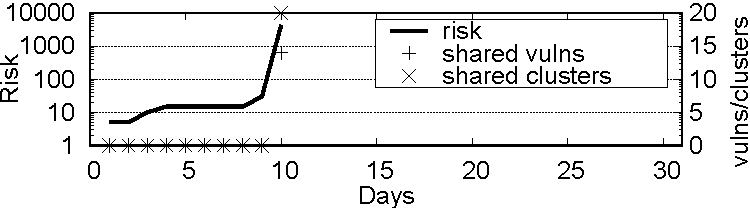
\includegraphics[width=0.5\columnwidth]{images/gnuplot/score/score_random_all.pdf}\label{fig:random_all}}
\hspace{0.5cm}
\subfloat[\system]{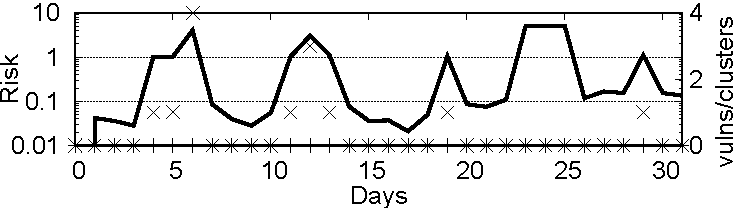
\includegraphics[width=0.5\columnwidth]{images/gnuplot/score/score_final_all.pdf}\label{fig:intel_all}}
\caption{Execution phase for Random and \system OS configuration strategies (log scale).}
\label{fig:run_all}
\end{figure*}

\textbf{Results:} As shown in Figure~\ref{fig:random_all}, \emph{Random} survives only for $10$ days. 
The number of shared clusters and vulnerabilities remains small for the first days. 
Then, there is a replica replacement that adds to the configuration an OS that has common vulnerabilities with the others. 
%Thus, enabling an adversary to compromise enough replicas in the system.

\system survives until the end of the experiment, as the risk is continually managed to keep the system safe. Figure~\ref{fig:intel_all} shows that shared clusters sometimes increase, at the same pace as the risk.
But then, the next reconfigurations are carried out with the goal of decreasing the risk. 
Notice that the risk value is always under $1$ for \system, and in the \emph{Random} is mostly above $10$.


\subsection{Diversity vs Attacks}

\begin{table}[t]
\begin{center}
{%\small%
\footnotesize
\begin{tabular}{ | p{0.96\columnwidth} | }\hline

\textbf{Samba:} 
\emph{On February 2, 2017, security researchers published details about a zero-day vulnerability in Server Message Block (SMB) of Windows, affecting several versions such as 8.1, 10, Server 2012 R2, and Server 2016. 
Could cause a \gls{dos} condition when a client accesses a malicious SMB.}\\
\textbf{CVES:} 
CVE-2017-0016
\\ \hline

\textbf{Wanna Cry:} 
\emph{On Friday, May 12, 2017, the world was alarmed to discover a widespread ransomware attack that hit organizations in more than 100 countries. Based on a vulnerability in Windows' SMB protocol (nicknamed EternalBlue), discovered by the NSA and leaked by Shadow Brokers.} \\
\textbf{CVES:} 
CVE-2017-0143, CVE-2017-0144, CVE-2017-0145, CVE-2017-0146, CVE-2017-0147, CVE-2017-0148 \\ \hline

\textbf{PowerShell:} 
\emph{Security feature bypass vulnerabilities in Device Guard that could allow an attacker to inject malicious code into a Windows PowerShell session.} \\
\textbf{CVES:}
CVE-2017-0219, CVE-2017-0173, CVE-2017-0215, CVE-2017-0216, CVE-2017-0218\\ \hline

\textbf{Stackclash:} 
\emph{In its 2017 malware forecast, SophosLabs warned that attackers would increasingly target Linux. The flaw, discovered by researchers at Qualys, is in the memory management of several operating systems and affects Linux, OpenBSD, NetBSD, FreeBSD and Solaris.}\\
\textbf{CVES:}
CVE-2017-1000365, CVE-2017-1000366, CVE-2017-1000367, CVE-2017-1000369, CVE-2017-1000370, CVE-2017-1000370, CVE-2017-1000371, CVE-2017-1000372, CVE-2017-1000373, CVE-2017-1000374, CVE-2017-1000375, CVE-2017-1000376, CVE-2017-1000379, CVE-2017-1083, CVE-2017-1084, CVE-2017-3629, CVE-2017-3630, CVE-2017-3631\\ \hline

\end{tabular}
}
\caption{Notable attacks during 2017.}
\label{tab:special_vulns}
\end{center}
\end{table}

This experiment evaluates the strategies when facing notable attacks/vulnerabilities that appeared in $2017$. 
Each attack potentially exploits several flaws, some of which affecting different \glspl{os}. 
The attacks were selected by searching the security news sites for high impact problems, most of them related to more than one CVE. 
As some of the \glspl{cve} include applications, we added more vulnerabilities to the database for this purpose.
Table~\ref{tab:special_vulns} lists the attacks and related \glspl{cve}: Samba,\footnote{https://www.secureworks.com/blog/attacking-windows-smb-zero-day-vulnerability} WannaCry,\footnote{https://securityintelligence.com/wannacry-ransomware-spreads-across-the-globe-makes-organizations-wanna-cry-about-microsoft-vulnerability/} Powershell,\footnote{http://blog.talosintelligence.com/2017/06/ms-tuesday.html} and Stackclash.\footnote{https://nakedsecurity.sophos.com/2017/06/20/stack-clash-linux-vulnerability-you-need-to-patch-now/}


Since some of these attacks might have been prepared months before the vulnerabilities are publicly disclosed, we augmented the execution phase to the full six months. 
As before, the strategies are analyzed over $5000$ runs.


\begin{figure}[t]
\begin{center}
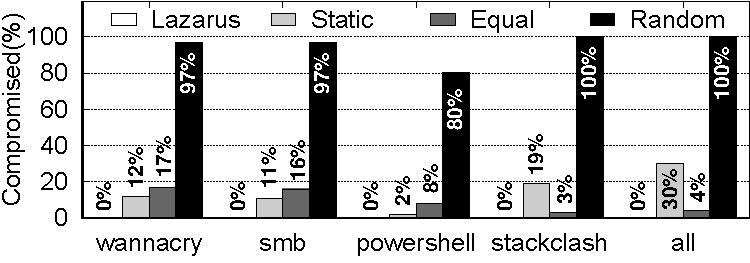
\includegraphics[width=\columnwidth]{images/gnuplot/special_vulns/execution-special.pdf}
\caption{Compromised runs with notable attacks.}
\label{fig:special_vulns}
\end{center}
\end{figure}

\textbf{Results:}
Figure~\ref{fig:special_vulns} shows the percentage of compromised runs for each attack and all attacks put together.
\system is clearly the best at handling the various scenarios, with no compromised executions.
\emph{Random} is the worse, as it does not use any criteria to select the OSes. 
Both \emph{Equal} and \emph{Static} may perform not so bad as they are static, i.e., the \glspl{os} selected by random chance might end up not being exploitable until the end of the run.

\section{Final Remarks}
\label{sec:finalremarkslazarus}

\system addresses the long-standing open problem of evaluating, selecting, and managing the diversity of a \gls{bft} system to make it resilient to malicious adversaries.
Our work focuses on two fundamental issues: how to select the best replicas to run together given the current threat landscape, and what is the performance overhead of running a diverse \gls{bft} system in practice.


\chapter{\system Implementation}
\label{chap:lazarus_implementation}

\chapter{\sieveq}
\label{chap:sieveq}

\chapter{Conclusion and Future Research Directions}
\label{chap:conclusion}

\section{Summary of the Results}
\system addresses the long-standing open problem of evaluating, selecting, and managing the diversity of a BFT system to make it resilient to malicious adversaries.
Our work focuses on two fundamental issues: how to select the best replicas to run together given the current threat landscape, and what is the performance overhead of running a diverse BFT system in practice.
Our results open many avenues for future work on this topic.

\paragraph{OS vulnerability Study}
The main results could be summarized as follows:
\begin{enumerate}
\item In most diverse \gls{os} configurations, significant  benefits in security could be observed: a low number of vulnerabilities were found to affect more than one \gls{os};

\item The number of vulnerabilities that affect more than one \gls{os} depends on how diverse the configuration is: they are higher for OSes from the same family (e.g., BSD) but very low (and in many cases zero) in OSes from different families (e.g., BSD and Windows);

\item We presented several strategies for system designers to choose most diverse \glspl{os} using \gls{nvd} data depending on whether they: consider all common vulnerabilities as being of equal importance; place greater emphasis on more recent common vulnerabilities (and hence wish to minimise the number of those); are primarily interested in the common vulnerabilities being reported less frequently in calendar time (which would allow them more time to respond to them). Surprisingly, for our dataset, all three strategies delivered the same best combination of four \glspl{os} for an intrusion-tolerant configuration (four being the usual number of systems needed to tolerate a Byzantine failure in a replicated system), which is: \textit{\{OpenBSD, Debian, Solaris, Windows2003\}}.

\end{enumerate}



\section{Future Work}

\textbf{Pretest replicas:}
Run a battery of tests (like Fuzzing, vulnerability detectors etc) before the system is running.

\textbf{Use vulnerable clone decttors on Opens source software to aggravete pairs with more clones} with dependcy graphs and autidting tools~\cite{Kim:2017}

\textbf{Test diversity agains automatic attacks, sometimes it may not be perfact, as the attacks we expect to see are APTs, however the idea is to verify if it takes more time to attack a replicated system with diversity}~\cite{Hu:2015}

\textbf{Vulnreabilities in the black market as a inditicar of severity}~\cite{Allodi:2014}.

\textbf{Virtualization technology:}
\system paid a performance penalty due to the limitations of the virtualization platform we used (VirtualBox).
VirtualBox was selected because it was the platform we could run more OSes.
Therefore its use enabled \system to support 17 different OSes for running BFT systems.
It would be great to have a VM technology capable of supporting all existing OSes without the resource limitations we experienced.

\textbf{Distributed control plane:}
As in previous works~\cite{Roeder:2010,Platania:2014}, our current design for \system considers a centralized trusted control plane that analyzes OSINT and orchestrates replica set reconfigurations.
It would be desirable to have a distributed version of such control plane, not only for improving its dependability but also to support the existence of multi-domain applications, such as blockchain platforms.

\textbf{Trusted components:}
Our prototype implements the LTU as a trusted component isolated from the rest of the replica in a VM, as many works on hybrid BFT~\cite{Veronese:2013,Roeder:2010,Platania:2014,Sousa:2010,Distler:2011}.
The recent popularization of trusted computing technologies such as Intel SGX~\cite{sgx}, and its use for implementing efficient BFT replication~\cite{Behl:2017}, open interesting possibilities for using novel hardware to support services like \system on bare metal.

\textbf{Integration with other sensors:}
\system monitors only five security data feeds on the internet looking for vulnerabilities, exploits, and patches in the OSes it manages, but it could be extended to monitor other indicators of compromise (e.g., IP black lists) extracted from a much richer set of sources~\cite{Liao:2016,Sabottke:2015}.
Similarly, \system can be extended to additionally use the outputs of IDSes to assess the BFT system behavior and trigger replica reconfigurations in case of need.

\textbf{Diversity-aware replication:}
The evaluation of BFT-SMaRt on top of \system shows that different replica set configurations can impact on the performance of applications, mostly due to the performance heterogeneity of the different OSes.
It would be interesting to consider protocols in which this heterogeneity is taken into account.
For example, the leader could be allocated in the fastest replica, or weighted-replication protocols such as WHEAT~\cite{Sousa:2015} could be used to assign higher weights to the replicas running in faster replicas.




% Fim do conteudo
% ----------------------------------------------------------------------

% Glossario

%
% Para actualizar o glossario, e' preciso correr o script ./fazindice
% e voltar a gerar o PDF
%
\LIMPA
\renewcommand{\glossaryname}{Acronyms}

\newacronym{aslr}{ASLR}{Address Space Layout Randomization}
\newacronym{arff}{ARFF}{Attribute-Relation File Format}
\newacronym{apts}{APTs}{Advanced Persistent Threats}



\newacronym{bft}{BFT}{Byzantine Fault Tolerance}
\newacronym{bm}{BM}{Bare Metal}

\newacronym[plural=CVEs,firstplural=Common Vulnerabilities and Exposures (CVEs)]{cve}{CVE}{Common Vulnerabilities and Exposures}
\newacronym{cpe}{CPE}{Common Platform Enumeration}
\newacronym{cvi}{CVI}{Common Vulnerability Indicator}
\newacronym{cvcs}{CVCst}{Common Vulnerability Count Strategy}
\newacronym{cvc}{CVC}{Common Vulnerability Count}
\newacronym{cvis}{CVIst}{Common Vulnerability Indicator Strategy}
\newacronym{irt}{IRT}{Inter-Reporting Times}
\newacronym{irts}{IRTst}{Inter-Reporting Times Strategy}
\newacronym{ip}{IP}{Internet Protocol}

\newacronym[plural=GPUs,firstplural=Graphics Processing Units (GPUs)]{gpu}{GPU}{Graphics Processing Unit}
\newacronym[plural=FPGAs,firstplural=Field-Programmable Gate Arrays (FPGAs)]{fpga}{FPGA}{Field-Programmable Gate Array}


\newacronym{cvss}{CVSS}{Common Vulnerability Scoring System}
\newacronym{xss}{XSS}{Cross-site scripting}


\newacronym{cots}{COTS}{Components Off-the-Shelf}
\newacronym{cis}{CIS}{CRUTIAL Information Switch}
\newacronym{dos}{DoS}{Denial-of-Service}
\newacronym{ddos}{DDoS}{Distributed Denial-of-Service}
\newacronym{dbms}{DBMS}{Databases Management Systems}
\newacronym{dns}{DNS}{Domain Name System}

\newacronym[plural=DBs,firstplural=Databases (DBs)]{db}{DB}{Database}

\newacronym{hmac}{HMAC}{Hash-based Message Authentication Code}


\newacronym{jvm}{JVM}{Java Virtual Machine}
\newacronym{ics}{ICS}{Industrial Control Systems}

\newacronym{ots}{OTS}{Off-the-Shelf}
\newacronym{osi}{OSI}{Open Systems Interconnection}

\newacronym[plural=OSes,firstplural=Operating Systems (OSes)]{os}{OS}{Operating System}
\newacronym[plural=IDSs,firstplural=Intrusion Detection Systems (IDSs)]{ids}{IDS}{Intrusion Detection System}


\newacronym{sql}{SQL}{Structured Query Language}

\newacronym[plural=MACs,firstplural=Message Authentication Codes (MACs)]{mac}{MAC}{Message Authentication Code}

\newacronym{nist}{NIST}{National Institute of Standards and Technology}
\newacronym{nvd}{NVD}{National Vulnerability Database}
\newacronym{nfs}{NFS}{Network File System}


\newacronym{ltu}{LTU}{Logical Trusted Unit}

\newacronym{scada}{SCADA}{Supervisory Control and Data Acquisition}
\newacronym{smr}{SMR}{State Machine Replication}
\newacronym{siem}{SIEM}{Security Information and Event Management}

\newacronym{udp}{UDP}{User Datagram Protocol}

\newacronym{ycsb}{YCSB}{Yahoo! Cloud Serving Benchmark}



\newacronym{osint}{OSINT}{Open Source Intelligence}
\newacronym{osvdb}{OSVDB}{Open Sourced Vulnerability Database}

\newacronym{tom}{TOM}{Total Ordered Multicast}
\newacronym{tls}{TLS}{Transport Layer Security}


\newacronym{mtd}{MTD}{Moving Target Defense}


\newacronym{po}{PO}{Proactive Obfuscation}

\newacronym{pr}{PR}{Proactive Recovery}
\newacronym{prr}{PRR}{Proactive-Reactive Recovery}
\newacronym{prrw}{PRRW}{Proactive-Reactive Recovery Wormhole}

\newacronym{zda}{ZDA}{Zero-Day Attack}
\newacronym{pzda}{PZDA}{Pseudo Zero-Day Attack}
\newacronym{ppzda}{PPZDA}{Potential Pseudo Zero-Day Attack}
\newacronym{poa}{POA}{Potential for Attack}


\newacronym{rsa}{RSA}{Rivest–Shamir–Adleman}
\newacronym{kvs}{KVS}{Key-Value Storage}
\newacronym{kmp}{KMP}{Knuth–Morris–Pratt}


\newacronym{svm}{SVM}{Support Vector Machines}
\newacronym{scit}{SCIT}{Self-Cleaning Intrusion Tolerance}

\newacronym{sha}{SHA}{Secure Hash Algorithm }

\newacronym{tcp}{TCP}{Transmission Control Protocol}
\newacronym{wine}{WINE}{Worldlwide Intelligence Network Environmnet}


\newacronym[plural=VMs,firstplural=Virtual Machines (VMs)]{vm}{VM}{Virtual Machine}
\newacronym{vmm}{VMM}{Virtual Machine Manager}
\newacronym{vpn}{VPN}{Virtual Private Network}

\newacronym{xml}{XML}{Extensible Markup Language}




\printglossaries
\addcontentsline {toc} {chapter} {Acronyms}
% Bibliografia

\LIMPA
\bibliographystyle{abbrv}
\bibliography{chapters/references/references}
%\addcontentsline {toc} {chapter} {Bibliography}

\end{document}
